\documentclass[
  10pt,
  hyperref={pdfauthor={William C. Dawn},
  pdftitle={Fast Reactor with FEM Multiphysics},
  pdfcreator={pdftex},
  pdfsubject={NC State Defense},
  pdfkeywords={nuclear, sodium, fast, reactor, nuclear reactor, 
    finite element, multiphysics},
%  colorlinks=true,
%  linkcolor=black,
%  citecolor=black,
%  filecolor=black,
%  urlcolor=black,
  }
]{beamer}
%\documentclass[handout,12pt]{beamer} % includes notes
\usetheme{NCSU}

\usepackage{amsmath,amsfonts,amssymb}
\usepackage{newtxtext}
\usepackage{microtype}
\usepackage[scaled=0.8]{newtxmath}

\usepackage[
			style=alphabetic,%numeric-comp,%authoryear-comp,%
			sorting=nyt,%ynt					
			hyperref=true, %	
			giveninits=true,%
			backend=bibtex,
			natbib=true,
			url=false,
			isbn=false,
			maxnames=2, %for et al to be used
			maxalphanames=1, %to avoid printing a + for every et al in abbreviation
			doi=false,
]{biblatex}		
\addbibresource{../WilliamDawn-thesis.bib}
\renewcommand*{\labelalphaothers}{}
\renewcommand*{\bibfont}{\scriptsize}
\setbeamertemplate{bibliography item}{\insertbiblabel}

\usepackage{booktabs,csvsimple,threeparttable}

% demand a table of contents for each current section
\AtBeginSection[]
{
  \begin{frame}
    \frametitle{Outline}
    \tableofcontents[currentsection]
  \end{frame}
}

% graphics packages
\usepackage{graphicx,subfig}
\def\Put(#1,#2)#3{\leavevmode\makebox(0,0){\put(#1,#2){#3}}}
% Remove "Figure: " and subfigure labels. decrease font size.
\captionsetup[subfigure]{labelformat=empty,font=scriptsize,labelfont=scriptsize}
\captionsetup{labelformat=empty,labelsep=none,font=scriptsize}
\usepackage[outdir=../hidden_epstopdf/]{epstopdf}
\graphicspath{
  {../ch01_introduction/figs/}
  {../ch02_neutronDiffusion/figs/}
  {../ch03_diffusionResults/figs/}
  {../ch04_thermalHydraulics/figs/}
  {../ch05_thermalExpansion/figs/}
  {../ch06_coupledResults/figs/}
  {../ch07_conclusions/figs/}
  {../apA_analyticSolutions/figs/}
  {../apB_benchmarks/figs/}
}

\usepackage{algorithm}
\usepackage[noend]{algpseudocode}
\algrenewcommand\alglinenumber[1]{\tiny #1:}
\makeatletter
\renewcommand{\ALG@beginalgorithmic}{\scriptsize}
\makeatother
\captionsetup[algorithm]{font=scriptsize}

\usepackage[acronym]{glossaries}
\usepackage{acronym}
\setacronymstyle{long-short}
\makeglossaries

\newacronym{fem}   {FEM}   {Finite Element Method}
\newacronym{spd}   {SPD}   {Symmetric Positive Definite}
\newacronym{sor}   {SOR}   {Successive Over-Relaxation}
\newacronym{cg}    {CG}    {Conjugate Gradient}
\newacronym{ebr-i} {EBR-I} {Experimental Breeder Reactor I}
\newacronym{ebr-ii}{EBR-II}{Experimental Breeder Reactor II}
\newacronym{vtr}   {VTR}   {Versatile Test Reactor}
\newacronym{inl}   {INL}   {Idaho National Laboratory}
\newacronym{sfr}   {SFR}   {Sodium-cooled Fast Reactor}
\newacronym{lwr}   {LWR}   {Light Water Reactor}
\newacronym{anl}   {ANL}   {Argonne National Laboratory}
\newacronym{geh}   {GEH}   {GE-Hitachi Nuclear Energy Americas LLC}
\newacronym{ulof}  {ULOF}  {Unprotected Loss-Of-Flow}
\newacronym{ulohs} {ULOHS} {Unprotected Loss-Of-Heat-Sink}
\newacronym{atws}  {ATWS}  {Anticipated Transient Without Scram}
\newacronym{lef}   {LEF}   {Linear Expansion Factor}
\newacronym{oecd}  {OECD}  {Organisation for Economic Co-operation and Development}
\newacronym{nea}   {NEA}   {Nuclear Energy Agency}
\newacronym{abr}   {ABR}   {Advanced Burner Reactor}
\newacronym{pcm}   {pcm}   {percent-mille ($10^{-5}$)}
\newacronym{ctc}   {CTC}   {Coolant Temperature Coefficient}
\newacronym{mtc}   {MTC}   {Moderator Temperature Coefficient}
\newacronym{cram}  {CRAM}  {Chebyshev Rational Approximation Method}
\newacronym{hwr}   {HWR}   {Heavy Water Reactor}
\newacronym{pwr}   {PWR}   {Pressurized Water Reactor}
\newacronym{fbr}   {FBR}   {Fast Breeder Reactor}
\newacronym{ornl}  {ORNL}  {Oak Ridge National Laboratory}
\newacronym{casl}  {CASL}  {Consortium for Advanced Simulation of LWRs}
\newacronym{iup}   {IUP}   {Integrated University Program}
\newacronym{doe-ne}{DOE-NE}{U.S. Department of Energy Office of Nuclear Energy}
\newacronym{spn}   {SP\textsubscript{N}}{Simplified $P_N$}
\newacronym{rcm}   {RCM}   {Reverse Cuthill-McKee}
\newacronym{rms}   {RMS}   {Root-Mean-Squared}

\glstocfalse
\renewcommand{\glossarysection}[2][]{}


% Information to be included in the title page:
\title[Fast Reactor and FEM]
  {Simulation of Fast Reactors with the Finite Element Method and Multiphysics 
  Models}
\author{William C. Dawn}
\institute{
  Nuclear Engineering Department \\
  North Carolina State University \\
  Raleigh, NC \\
  \texttt{\href{mailto:wcdawn@ncsu.edu}{wcdawn@ncsu.edu}}
}
\date{March 8, 2019}

% custom variable definitions
\usepackage{xspace}

% linear algebra
\renewcommand{\epsilon}{\varepsilon} % use the pretty epsilon

%    vectors
\newcommand{\va}{\mathbf{a}}
\newcommand{\vb}{\mathbf{b}}
\newcommand{\vc}{\mathbf{c}}
\newcommand{\vd}{\mathbf{d}}
\newcommand{\ve}{\mathbf{e}}
\newcommand{\vf}{\mathbf{f}}
\newcommand{\vp}{\mathbf{p}}
\newcommand{\vr}{\mathbf{r}}
\newcommand{\vu}{\mathbf{u}}
\newcommand{\vx}{\mathbf{x}}
\newcommand{\vw}{\mathbf{w}}
\newcommand{\vPhi}{\Phi}

%    matrices
\newcommand{\ma}{\mathbf{A}}
\newcommand{\mb}{\mathbf{B}}
\newcommand{\mj}{\mathbf{J}}
\newcommand{\ml}{\mathbf{L}}
\newcommand{\mm}{\mathbf{M}}
\newcommand{\mr}{\mathbf{R}}

%    sets
\newcommand{\real}{\mathbb{R}}
\newcommand{\realn}{\real^{n}}
\newcommand{\realnn}{\real^{n \times n}}

% variable definitions
\newcommand{\keff}{\ensuremath{k_{\!\mbox{\scriptsize \em eff}}}\xspace}
\newcommand{\keffsub}[1]{\ensuremath{k_{\!\mbox{\scriptsize \em eff,{#1}}}}}
\newcommand{\kref}{\ensuremath{k_{\!\mbox{\scriptsize \em ref}}}}
\newcommand{\grad}{\mathbf{\nabla}}

% neutronDiffusion
\newcommand{\albedo}{\alpha}
\newcommand{\basis}{N}
\newcommand{\twotable}{TwoTable }
\newcommand{\phiavg}{\overline{\phi}}
\newcommand{\nhat}{\hat{\mathbf{n}}}

% diffusionResults
\newcommand{\true}{\checkmark}

% code names
\newcommand{\dif}{\text{DIF3D}\xspace}
\newcommand{\mcc}{\text{MC**2}\xspace}

% thermalHydraulics
\newcommand{\mdot}{\dot{m}}

% thermalExpansion
\newcommand{\texp}
  {\ensuremath{{T_{\!\mbox{\scriptsize \em exp}}}}}
\newcommand{\texpfuel}
  {\ensuremath{{T_{\!\mbox{\scriptsize \em exp,fuel}}}}}
\newcommand{\texpstruct}
  {\ensuremath{T_{\!\mbox{\scriptsize \em exp,struct}}}}

% general macros
\newcommand{\units}[1]{\ensuremath{\left[\text{{#1}}\right]}}
\newcommand{\half}{\frac{1}{2}}
\newcommand{\nicesub}[2]{\ensuremath{{#1}_{\!\mbox{\scriptsize \em {#2}}}}}

% reference macros
\newcommand{\eref}[1]{Eq.~(\ref{#1})}
\newcommand{\fref}[1]{Fig.~\ref{#1}}
\newcommand{\tref}[1]{Table~\ref{#1}}
\newcommand{\sref}[1]{\S\ref{#1}}
\newcommand{\chref}[1]{Chapter~\ref{#1}}
\newcommand{\apref}[1]{Appendix~\ref{#1}}
\newcommand{\algorithmref}[1]{Algorithm~\ref{#1}}

\usepackage{array}
\newcolumntype{L}{>{$}l<{$}}
% \newenvironment{conditions}
%   {\par\vspace{\abovedisplayskip}\noindent\begin{tabular}{>{$}l<{$} @{${}={}$} l}}
%   {\end{tabular}\par\vspace{\belowdisplayskip}}
\newenvironment{conditions}
  {\par\noindent\begin{tabular}{L @{${}={}$} l}}{\end{tabular}\par}


\begin{document}

\begin{frame}
  \titlepage
\end{frame}

\section{} % syntax for an unnamed section
  \begin{frame}
    \frametitle{Disclaimer}
    \vspace*{\fill}
    \begin{center}
      \mbox{\parbox{0.7\textwidth}{
      This material is based upon work supported under an Integrated University 
      Program Graduate Fellowship. Any opinions, findings, conclusions, or 
      recommendations expressed in this publication are those of the author and 
      do not necessarily reflect the views of the Department of Energy Office of 
      Nuclear Energy.
      }}
    \end{center}
    \vspace*{\fill}
  \end{frame}

\begin{frame}
  \frametitle{Table of Contents}
  \tableofcontents
\end{frame}

\section{Introduction}
\label{sec:introduction}

\begin{frame}{Why are we here?}
  \pause
  \begin{itemize}
    \item Probably because I asked you to come.
    \item Or because a professor told you to come.
  \end{itemize}
\end{frame}

\begin{frame}{Why are we here?}
  \begin{itemize}
    \item {\huge Model a nuclear reactor.}
      \pause
      \begin{itemize}
        \item Neutron distribution.
        \item Thermal Hydraulics.
        \item Thermal Expansion.
      \end{itemize}
  \end{itemize}
\end{frame}

\begin{frame}{But it's already been done!}
  \begin{itemize}
    \pause 
    \item You're right.
    \pause
    \item Computers are different now.
    \item Mathematical methods are more efficient now.
    \item \textbf{FORTRAN} has \textit{a few} new standards.
  \end{itemize}
\end{frame}

\begin{frame}{\textit{Present} Simulation Procedure}
  \begin{itemize}
    \item Heuristically estimate material temperatures.
    \item Manually calculate thermally expanded dimensions.
    \item Manually calculate area fractions and number densities.
    \item Run \dif and get \keff and power distribution.
    \pause
    %\item \dif was last updated 1993. \textbf{FORTRAN} last updated 2008.
  \end{itemize}
  \vspace{0.3in}
  \begin{block}{}
    No thermal feedback capability. Modern numerical methods can be
    implemented.
  \end{block}
\end{frame}

\begin{frame}{Goals}
  \begin{itemize}
    \item User input.
      \begin{itemize}
        \item Easy to use.
        \item Reactor geometry via \texttt{VTK} mesh.
        \item Temperature dependent cross-sections either plain-text or 
          \texttt{ISOTXS}.
        \item Pin dimensions and material compositions.
      \end{itemize}
    \item Simulate thermal expansion and thermal hydraulics internally.
    \item Collect \keff, reactor power, and average material temperatures.
  \end{itemize}
  \vspace{0.25in}
  \begin{itemize}
    \item Thermal expansion and thermal hydraulic simulations have been moved
      internally and are now inherent to the simulation.
    \item Thermal hydraulic simulation also improves the accuracy of neutronics
      simulation by leading to more accurate cross sections.
  \end{itemize}
\end{frame}

\begin{frame}{Geometry Description}
  \begin{itemize}
    \item Hexagonal.
    \item Boxed assemblies.
    \item Resolve individual assemblies and specified elevations.
  \end{itemize}
\end{frame}

\begin{frame}{Fuel Rod}
  \begin{figure}
    \centering
    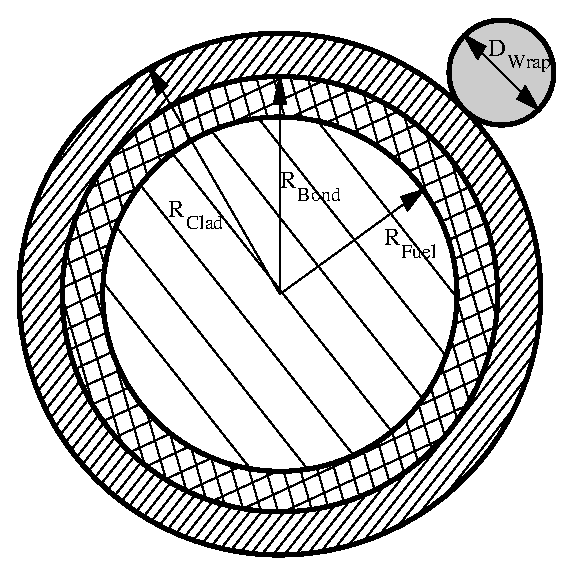
\includegraphics[width=0.5\textwidth]{pin_model}
    %\caption{Dimensions of Thermal Hydraulic Rod Model.}
    \label{fig:pin_model}
  \end{figure}
\end{frame}

\begin{frame}{Hexagonal Assembly}
  \begin{figure}
    \centering
    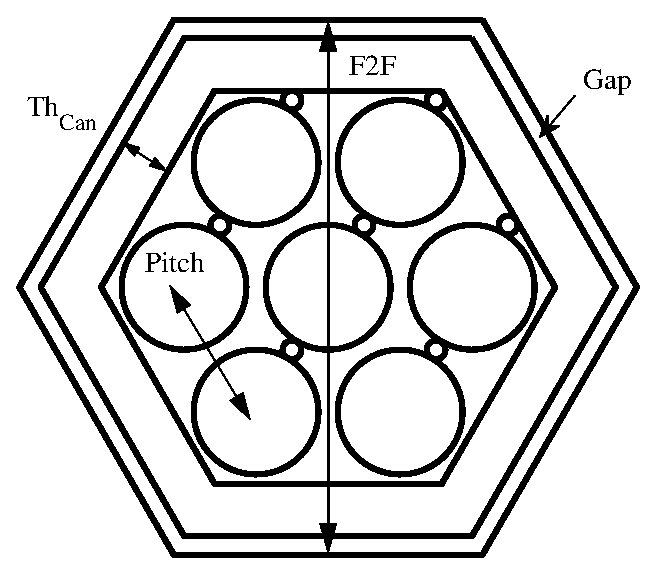
\includegraphics[width=0.5\textwidth]{hex_can}
    %\caption{Dimensions of Hexagonal Can.}
    \label{fig:hex_can}
  \end{figure}
\end{frame}

\begin{frame}{Fuel Assembly}
  \begin{figure}
    \centering
    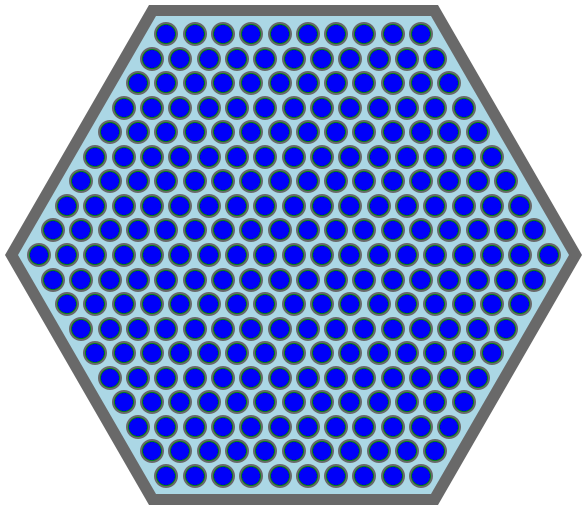
\includegraphics[width=0.5\textwidth]{prism_hex}
    \caption{Example of Fast Reactor Fuel Assembly Cross-section with 217 rods.}
    \label{fig:prism_hex}
  \end{figure}
\end{frame}

\begin{frame}
  \begin{figure}
    \centering
    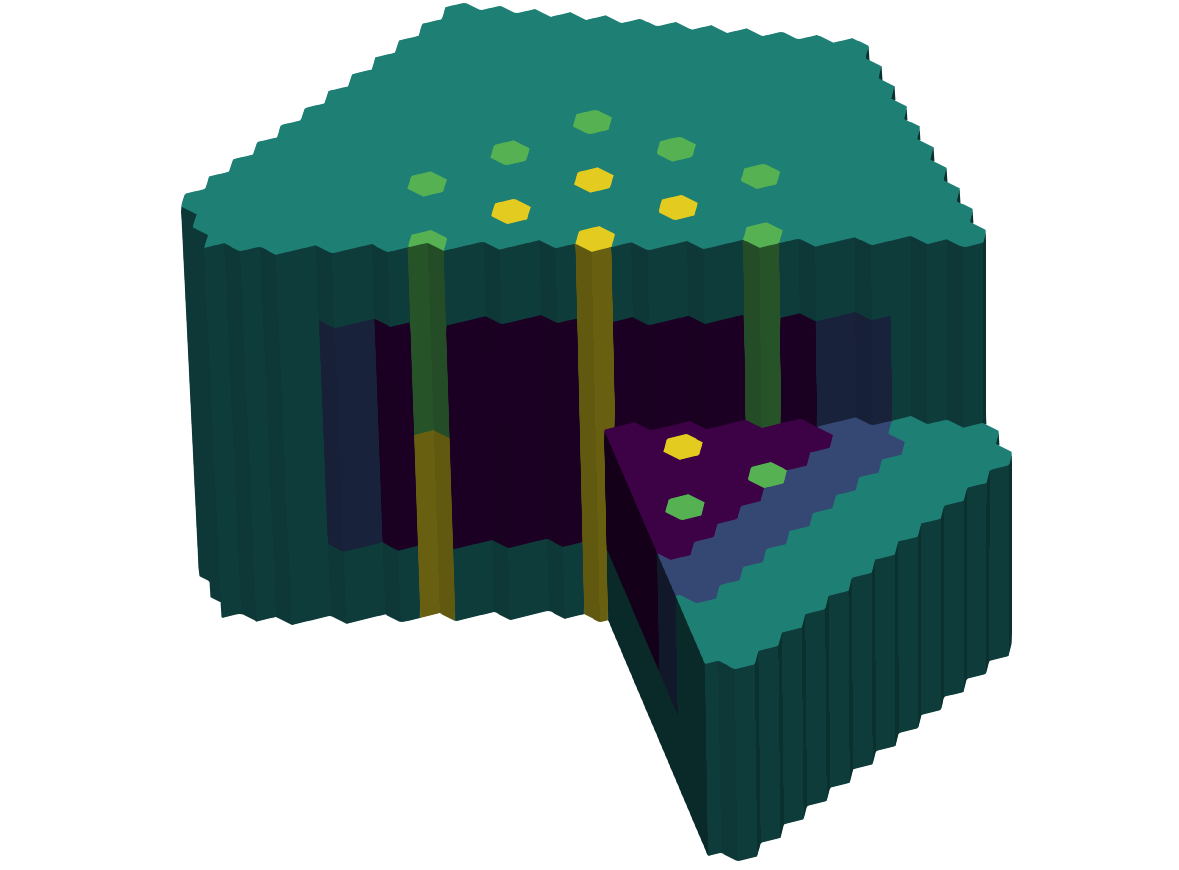
\includegraphics[width=0.9\textwidth]{reactor_materials}
    \caption{Example of Fast Reactor Materials based on MONJU.}
    \label{fig:reactor_materials}
  \end{figure}
\end{frame}

\chapter{Finite Element Neutron Diffusion}
\label{ch:neutronDiffusion}

\section{Introduction}
  This chapter will describe the solution of the multigroup neutron diffusion
  equations for general geometry via the \glsentryfull{fem}. The solution method
  and derivations here are general to the multigroup neutron diffusion equation
  and its application to any standard reactor geometry is straightforward. For
  typical fast reactor applications, diffusion theory approximates the neutron
  distribution within the reactor well. The diffusion approximation is a
  standard assumption for fast reactors because neutron mean-free-paths within
  the reactor are large relative to material dimensions.

  Spatial discretization will be done with the \gls{fem}. This spatial 
  discretization method is selected for several reasons. It allows for easily 
  increasing the spatial convergence order of the method by increasing the order
  of the elements without refining the mesh. For example, with a given mesh, 
  quadratic elements instead of linear elements could be used to spatially 
  refine the solution. Additionally, coordinates of nodes and elements can be 
  easily updated to reflect physical phenomena, such as thermal expansion (see 
  \chref{ch:thermalExpansion}). Finally, material properties are calculated on 
  an element basis allowing for detailed updates to the material properties 
  during the calculation.

\section{Multigroup Neutron Diffusion Equation}
  In the multigroup neutron diffusion equation, an energy structure is 
  described by the set of energies $\{E_g\}$ for $g = 1,2,\ldots,G$.
  By convention, the energy groups are arranged in order of decreasing energy.
  \begin{equation}
    0 < E_G < E_{G-1} < \ldots < E_2 < E_1
  \end{equation}
  Multigroup neutron cross sections can be calculated using this energy group 
  structure from energy dependent cross sections, and a representative flux
  spectrum. Generation of multigroup neutron cross sections is performed using
  \mcc and is described in \sref{sec:cross_section_treatment}.

  In conventional notation, the multigroup neutron diffusion equation can be
  written as 
  \begin{equation}
    \label{eq:multigroup_diffusion}
    - \grad \cdot ( D_g(\vr) \grad \phi_g(\vr)) + \Sigma_{t,g}(\vr) \phi_g(\vr)= 
      \frac{\widetilde{\chi_g}(\vr)}{\keff} 
      \sum_{g'=1}^{G} \nu\Sigma_{f,g'}(\vr) 
      \phi_{g'}(\vr) + \sum_{g'=1}^{G} \Sigma_{s,g' \rightarrow g}(\vr) 
      \phi_{g'}(\vr)
  \end{equation}
  where 
  \begin{conditions} % custom environment designed for this purpose
    \vr & spatial position vector, \\
    D_g(\vr)    & diffusion coefficient for energy group $g$ \units{cm}, \\
    \phi_g(\vr) & scalar neutron flux for energy group $g$
      \units{$\frac{1}{\text{cm}^2 \; \text{s}}$}, \\
    \Sigma_{t,g}(\vr) & macroscopic total cross section for energy group $g$ 
      \units{$\frac{1}{\text{cm}}$}, \\
    \widetilde{\chi_g}(\vr) & effective fission spectrum for energy group $g$,\\
    \keff & effective neutron multiplication factor, \\
    \nu \Sigma_{f,g}(\vr) & number of fission neutrons times microscopic fission
      cross section in energy group $g$ \units{$\frac{1}{\text{cm}}$}, \\
    \Sigma_{s,g' \rightarrow g} (\vr) & macroscopic scatter cross section from
      energy group $g'$ to energy group $g$ \units{$\frac{1}{\text{cm}}$}, \\
    G & total number of energy groups.
  \end{conditions}

  The total neutron cross section includes the contribution due to within-group
  scattering; that is, due to $\Sigma_{s,g\rightarrow g}$. This can be
  subtracted from both sides of \eref{eq:multigroup_diffusion} for simplicity
  and numeric efficiency. Rewriting \eref{eq:multigroup_diffusion} with this
  modification yields
  \begin{equation} 
    \label{eq:multigroup_removal}
    - \grad \cdot( D_g(\vr) \grad \phi_g(\vr)) + \Sigma_{r,g}(\vr) \phi_g(\vr) = 
      \frac{\widetilde{\chi_g}(\vr)}{\keff} 
      \sum_{g'=1}^{G} \nu\Sigma_{f,g'}(\vr) 
      \phi_{g'}(\vr) + \sum_{g'=1, g' \ne g}^{G} 
      \Sigma_{s,g' \rightarrow g}(\vr) \phi_{g'}(\vr)
  \end{equation}
  where $\Sigma_{r,g}$ is the removal cross section defined as
  $\Sigma_{r,g}(\vr) = \Sigma_{t,g}(\vr) - \Sigma_{s,g\rightarrow g}(\vr)$. The
  removal cross section now describes the removal of neutrons from the element
  of phase space due to nuclear interactions.  For simplicity, the neutron
  sources in \eref{eq:multigroup_removal} can be combined into a single term as
  \begin{equation}
    \label{eq:multigroup_source}
    - \grad \cdot( D_g(\vr) \grad \phi_g(\vr)) + \Sigma_{r,g}(\vr) \phi_g(\vr) = 
      q_g(\vr)
  \end{equation}
  where $q_g(\vr)$ is the combined neutron source at position $\vr$ for energy
  group $g$ and is expressed as
  \begin{equation}
    \label{eq:q}
    q_g(\vr) = q_{fiss,g}(\vr) + q_{up,g}(\vr) + q_{down,g}(\vr) 
  \end{equation}
  with contributing terms
  \begin{align}
    \label{eq:qfiss}
    q_{fiss,g}(\vr) &= \frac{\widetilde{\chi_g}(\vr)}{\keff} \sum_{g'=1}^{G} 
      \nu \Sigma_{f,g'}(\vr) \phi_{g'}(\vr), \\
    \label{eq:qup}
    q_{up,g}(\vr) &= \sum_{g'=g+1}^{G} \Sigma_{s,g' \rightarrow g}(\vr)
      \phi_{g'}(\vr), \\
    \label{eq:qdown}
    q_{down,g}(\vr) &= \sum_{g'=1}^{g-1} \Sigma_{s,g' \rightarrow g}(\vr)
      \phi_{g'}(\vr),
  \end{align}
  where the difference between $q_{up}$ and $q_{down}$ are the limits of the
  summation. $q_{up}$ represents the neutron source due to scattering from lower
  energy groups (up-scattering) and $q_{down}$ represents the neutron source due
  to scattering from higher energy groups (down-scattering). This form allows
  for operator splitting of the neutron source term. In an iterative scheme, it
  will be necessary for fission and up-scatter sources to use a different flux
  iterate than down-scatter so this separation of sources will prove useful (see
  \sref{sec:calculation_of_source_with_power_iterations}).

  The combined source form is useful for solving the multigroup neutron
  diffusion problem for an arbitrary number of groups.
  \eref{eq:multigroup_source} is solved for each energy group and interaction
  between groups is described in the source term, $q_g(\vr)$. In other
  literature, the multigroup equation may be solved for all groups
  simultaneously by treating interaction between groups explicitly. By solving
  each group independently (as done here) the method remains general.
  Additionally, for many-group energy structures, as common to fast reactor
  applications, solving each group independently is typically more
  computationally efficient as such linear systems have favorable conditioning
  and are dimensionally smaller. Finally, fast reactors are also dominated by
  down-scatter as opposed to thermal reactors which experience significant
  up-scatter implying that the term $q_{up,g}(\vr)$ will not have to be updated
  frequently and the one group at-a-time solution method will benefit.

  Typically, reactor materials are described isotopically and $\chi$ may be
  specified isotopically. However, for calculating the fission neutron source
  $q_{fiss,g}(\vr)$ as in \eref{eq:qfiss}, an effective $\widetilde{\chi}$ is 
  needed. From an isotopic description, $q_{fiss,g}(\vr)$ is given as
  \begin{equation}
    \label{eq:isotopic_chi}
    q_{fiss,g}(\vr) = \sum_{i=1}^{N_{iso}} \chi_{i,g}(\vr)
      \nu \Sigma_{f,i,g}(\vr) \phi_g(\vr)
  \end{equation}
  where $\chi_{i,g}(\vr)$ is the isotopic fission spectrum and $N_{iso}$ is the 
  number of isotopes at position $\vr$. Next, require $q_{fiss,g}(\vr)$ to have 
  the form of \eref{eq:element_chi}.
  \begin{equation}
    \label{eq:element_chi}
    q_{fiss,g}(\vr) = \widetilde{\chi_g}(\vr) \, 
      \sum_{i=1}^{N_{iso}} \nu \Sigma_{f,i,g}(\vr) \phi_g(\vr)
  \end{equation}
  Setting \eref{eq:isotopic_chi} equal to \eref{eq:element_chi} yields the
  expression for $\widetilde{\chi_g}(\vr)$ based on isotopic data.
  \begin{equation}
    \label{eq:chi_collapse}
    \widetilde{\chi_g}(\vr) = \frac{\sum_{i=1}^{N_{iso}} \chi_{i,g}(\vr)
      \nu \Sigma_{f,i,g}(\vr) \phi_g(\vr)}
      {\sum_{i=1}^{N_{iso}} \nu \Sigma_{f,i,g}(\vr) \phi_g(\vr)}
  \end{equation}
  Note that \eref{eq:chi_collapse} requires the solution $\phi_g(\vr)$.
  Ultimately, the flux is unknown but will be solved in an iterative manner.
  \eref{eq:chi_collapse} implies that $\widetilde{\chi_g}(\vr)$ must be updated
  for each iteration of the solution (see Step \ref{state:chi_collapse} in
  \algorithmref{algorithm:general}).
  
\section{Formulation of Finite Element Equations}
  \label{sec:formulation}
  This section presents the derivation of the spatial discretization of the
  multigroup neutron diffusion equation based on the \gls{fem}. The method
  results in a linear system of equations for a fixed source iteration. Details
  are also provided on constructing the finite element matrix for use with
  triangular and wedge elements.

  \subsection{Derivation}
    \label{sec:formulation:derivation}
    The remaining continuous variable in the problem to be discretized in
    \eref{eq:multigroup_source} is the spatial variable $\vr$. This will be 
    discretized according to the \gls{fem}. The problem is solved in a finite 
    domain $\vr \in \Omega$ where $\partial \Omega$ represents the boundary of 
    the domain and some boundary condition is specified. Boundary condition 
    options include:
    \begin{enumerate}
      \item Mirror. $\grad \phi_g(\vr) \cdot \nhat = 0$ for 
        $\vr \in \partial \Omega$.
      \item Albedo. $D_g(\vr) \grad \phi_g(\vr) \cdot \nhat + 
        \albedo \phi_g(\vr)=0$ for $\vr \in \partial \Omega$,
        where $\albedo \in \real$ is a scalar constant specified
        by the user. For non-reentrant boundary condition, $\albedo = \half$.
      \item Zero Flux. $\phi_g(\vr) = 0$ for $\vr \in \partial \Omega$.
    \end{enumerate}
    $\nhat$ represents the unit outward normal vector at the boundary $\partial
    \Omega$.
    (Note: the order of the above list corresponds to the order of boundary 
    condition precedent in code with the greater the integer, the greater the 
    precedent.)
    
    Begin by partitioning the spatial domain $\Omega$ into a set of finite 
    elements.
    \begin{equation}
      \label{eq:set_of_elements}
      \Omega = \Omega_1 \cup \Omega_2 \cup \Omega_3 \cup \ldots \cup
        \Omega_{N_E} 
    \end{equation}
    such that $\Omega = \{\Omega_e\}$ for $e = 1,2,\ldots,N_E$ is a set of
    non-overlapping elements 
    \begin{equation}
      \label{eq:non_overlapping}
      \Omega_i \cap \Omega_j = \emptyset, \quad \text{for } i \ne j
    \end{equation}
    and $N_E$ is the total number of elements. Elements are in an unstructured
    mesh and can be generated by any number of mesh generation methods (e.g.
    Delaunay triangulation) to describe the geometry of the problem.
    
    Proceeding with the Galerkin \gls{fem}, \eref{eq:multigroup_source} is
    multiplied by a testing function $v(\vr) \in H_1(\Omega)$ where $H$ is the
    Sobolev space. 
    \begin{equation}
      \label{eq:testing_function_multiply}
      -\grad \cdot (D_g(\vr) \grad \phi_g(\vr)) v(\vr) + 
        \Sigma_{r,g}(\vr) \phi_g(\vr) v(\vr) =
        q_g(\vr) v(\vr)
    \end{equation}
    Then, \eref{eq:testing_function_multiply} is integrated over the problem 
    domain. This integration yields the Weak Form or Variational Form of the 
    problem.
    \begin{equation}
      \label{eq:fem_weak_form}
      - \int_{\Omega} \grad \cdot (D_g(\vr) \grad \phi_g(\vr)) v(\vr) \; d\vr
        + \int_{\Omega} \Sigma_{r,g}(\vr) \phi_g(\vr) v(\vr) \;d\vr=
        \int_{\Omega} q_g(\vr) v(\vr) \;d\vr
    \end{equation}
    
    For the purposes of this work, material cross sections and the neutron
    source, $q_{g,e}$, are assumed to be constant within an element. In the
    future, $q_g$ could be considered discrete at each node rather than each
    element. To calculate a constant neutron source within an element,
    \eref{eq:q} is used to calculate the average neutron source, $q_{g,e}$,
    in an element.
    \begin{align}
      q_{g,e} &= q_{fiss,g,e} + q_{up,g,e} + q_{down,g,e} \\
      \label{eq:chielement}
      \widetilde{\chi_{g,e}} &= \frac{\sum_{i=1}^{N_{iso}} \chi_{i,g,e}
        \nu \Sigma_{f,i,g,e} \phiavg_{g,e}}
        {\sum_{i=1}^{N_{iso}} \nu \Sigma_{f,i,g,e} \phiavg_{g,e}} \\
      \label{eq:qelement_fiss}
      q_{fiss,g,e} &= \frac{\widetilde{\chi_{g,e}}}{\keff} \sum_{g'=1}^G \nu
        \Sigma_{f,g',e} \phiavg_{g',e} \\
      \label{eq:qelement_up}
      q_{up,g,e} &= \sum_{g'=g+1}^G \Sigma_{s,g' \rightarrow g,e}
        \phiavg_{g',e}\\
      \label{eq:qelement_down}
      q_{down,g,e} &= \sum_{g'=1}^{g-1} \Sigma_{s,g' \rightarrow g,e}
        \phiavg_{g',e}
    \end{align}
    Note that in \eref{eq:chielement}, $\widetilde{\chi_{g,e}}$ must now be
    calculated for each finite element.  For first-order, linear implementations
    of the \gls{fem}, the element-average flux $\phiavg_{g,e}$ is
    \begin{equation}
      \label{eq:phiavg}
      \phiavg_{g,e} = \frac{1}{N_p} \sum_{i \in \Omega_e}^{N_p} \phi_{i,g}
    \end{equation}
    where $N_p$ is the number of nodes on the element and $i \in
    \Omega_e$ is the summation over all nodes in element $\Omega_e$. For 
    example, a triangle has $N_p = 3$ and a wedge has $N_p = 6$.

    Given constant material properties and constant neutron source over the
    element, the integrals in \eref{eq:fem_weak_form} can be partitioned into a
    sum of integrals over the elements in the domain assuming the
    non-overlapping set of elements from \eref{eq:set_of_elements} and
    \eref{eq:non_overlapping}.
    \begin{equation} 
      \label{eq:element_by_element}
      -\sum_{e=1}^{N_E} D_{g,e} 
        \int_{\Omega_e} \grad \cdot \grad \phi_g(\vr) v(\vr) \; d\vr +
        \sum_{e=1}^{N_E} \Sigma_{r,g,e} \int_{\Omega_e} \phi_g(\vr) v(\vr) 
        \;d\vr = \sum_{e=1}^{N_E} q_{g,e} \int_{\Omega_e} v(\vr) 
        \; d\vr
    \end{equation}
    The Second Green's Theorem is used to rewrite the integral in the first
    term. A proof invoking the Second Green's Theorem has been published by
    \textcite{textbookli}. % in Theorem 9.2.
    The Second Green's Theorem is 
    \begin{equation} 
      \label{eq:greens}
      -\int_{\Omega_e} \grad \cdot \grad \phi_g(\vr) v(\vr) \;d\vr =
        -\int_{\partial \Omega_e}  
        (\grad \phi_g(\vr) \cdot \nhat) \, v(\vr)\; ds +
        \int_{\Omega_e} \grad \phi_g(\vr) \cdot \grad v(\vr) \; d\vr
    \end{equation}
    where $\grad \phi_g(\vr) \cdot \nhat$ is the outward normal derivative and
    the integral $\int_{\partial \Omega} {\cdot} \;ds$ is a line integral in two
    dimensions or a surface integral in three dimensions. Recognizing that this
    quantity will only be relevant on the boundary of the problem, the value of
    the outward normal derivative will be specified as a boundary condition.
    Specifically, the albedo boundary condition which has the form 
    \begin{align}
      D_g(\vr) \grad \phi_g(\vr) \cdot \nhat + \albedo \phi_g(\vr) &= 0 \\
      D_g(\vr) \grad \phi_g(\vr) \cdot \nhat &= -\albedo \phi_g(\vr)
    \end{align}
    for $\vr \in \partial \Omega$. Note that all allowed boundary conditions
    (mirror, albedo, and zero-flux) can be specified as an albedo condition. For
    mirror boundaries, $\albedo = 0$ and for zero-flux boundaries, $\albedo
    \rightarrow \infty$.  Substituting \eref{eq:greens} into
    \eref{eq:element_by_element} and assuming the outward normal derivative is
    specified in the form of an albedo boundary condition with $\albedo$
    constant throughout the problem boundary.
    \begin{multline} 
      -\sum_{e=1}^{N_E} D_{g,e} \int_{\partial \Omega_e} v(\vr) \grad
      \phi_g(\vr) \cdot \nhat \;ds + \sum_{e=1}^{N_E} 
        D_{g,e} \int_{\Omega_e} \grad \phi_g(\vr) \cdot \grad v(\vr) 
        \; d\vr + \\
        \sum_{e=1}^{N_E} \Sigma_{r,g,e} \int_{\Omega_e} \phi_g(\vr) v(\vr) 
        \; d\vr =
        \sum_{e=1}^{N_E} q_{g,e} \int_{\Omega_e} v(\vr) \; d\vr
    \end{multline}
    \begin{multline}
      \label{eq:element_boundary}
      \sum_{e=1}^{N_E} \albedo \int_{\partial \Omega_e} v(\vr) 
        \phi_g(\vr) \;ds + \sum_{e=1}^{N_E} D_{g,e}
        \int_{\Omega_e} \grad \phi_g(\vr) \cdot \grad v(\vr) \; d\vr + \\
        \sum_{e=1}^{N_E} \Sigma_{r,g,e} \int_{\Omega_e} \phi_g(\vr) v(\vr) 
        \; d\vr =
        \sum_{e=1}^{N_E} q_{g,e} \int_{\Omega_e} v(\vr) \; d\vr
    \end{multline}
    Next, for the Galerkin formulation of the \gls{fem}, the function of
    interest $\phi_g(\vr)$ is assumed to be a linear combination of chosen basis
    functions, $\basis_i$, as
    \begin{equation} 
      \label{eq:linear_combination}
      \phi_g(\vr) = \sum_{i=1}^{DOF} \upsilon_{i,g} \, \basis_i(\vr)
    \end{equation}
    where coefficients $\vu_g = \{\upsilon_{i,g}\}$ are unknown and will be 
    determined and $DOF$ is the total number degrees of freedom of the problem. 
    Typically $DOF$ is the number of nodes less any nodes for which the flux is 
    fixed (e.g. zero-flux nodes). 
    
    Typically, basis functions have unit magnitude and are centered at the node
    points so the coefficients $\upsilon_{i,g}$ are the \gls{fem} solution at the
    nodes. It is also convenient for basis functions to have compact support.
    That is, basis functions are created such that they are zero almost
    everywhere except some minimal region. Compact support in this
    implementation is chosen such that basis functions have unit value on a
    single mesh node and are zero on all other mesh nodes. Basis functions are
    typically piecewise continuous polynomials of arbitrary degree. For selected
    elements, basis functions will be defined explicitly in
    \sref{sec:matrix_quantities}. Linear and quadratic polynomials are common;
    but, for the work presented here, only linear basis functions are explored.

    The test function, $v(\vr) \in H_1(\Omega)$, is also chosen as a linear 
    combination of the same basis functions.
    \begin{equation} 
      \label{eq:linear_superposition}
      v(\vr) = \sum_{j=1}^{DOF} \basis_j(\vr)
    \end{equation}
    The magnitude of the testing function is arbitrary so the magnitude is set
    to unity.
    
    \eref{eq:linear_combination} and \eref{eq:linear_superposition} are inserted 
    into \eref{eq:element_boundary}.
    \begin{multline}
      \label{eq:this_above}
      \sum_{e=1}^{N_E} \albedo \sum_{i=1}^{DOF} \upsilon_{i,g}
        \int_{\partial \Omega_e}
        \basis_i(\vr)  \basis_j(\vr) \;ds +
        \sum_{e=1}^{N_E} D_{g,e} \sum_{i=1}^{DOF} \upsilon_{i,g}
        \int_{\Omega_e} \grad \basis_i(\vr) \cdot \grad \basis_i(\vr)\;d\vr
        + \\
        \sum_{e=1}^{N_E} \Sigma_{r,g,e} \sum_{i=1}^{DOF} \upsilon_{i,g}
        \int_{\Omega_e} \basis_i(\vr) \basis_j(\vr) \; d\vr =
        \sum_{e=1}^{N_E} q_{g,e} \sum_{i=1}^{DOF} 
        \int_{\Omega_e} \basis_i(\vr) \; d\vr
    \end{multline}
    \eref{eq:this_above} can be rearranged as a linear system of equations.
    \begin{multline}
      \label{eq:linear_equation}
      \sum_{i=1}^{DOF} \upsilon_{i,g} \sum_{j=1}^{DOF} \left(
        \sum_{e=1}^{N_E} \albedo \int_{\partial \Omega_e}
        \basis_i(\vr)  \basis_j(\vr) \;ds +
        \sum_{e=1}^{N_E} D_{g,e} 
        \int_{\Omega_e} \grad \basis_i(\vr) \cdot \grad \basis_j(\vr)\;d\vr
        \right.
        + \\
        \left.
        \sum_{e=1}^{N_E} \Sigma_{r,g,e}
        \int_{\Omega_e} \basis_i(\vr) \basis_j(\vr) \; d\vr \right) =
        \sum_{i=1}^{DOF} \left(
        \sum_{e=1}^{N_E} q_{g,e} 
        \int_{\Omega_e} \basis_i(\vr) \; d\vr \right)
    \end{multline}
    Which can be written in the notation common to the mathematical discussions 
    of the \gls{fem}
    \begin{equation}
      \label{eq:fem_notation}
      a_g(\basis_i,\basis_j) = f_g(\basis_i)
    \end{equation}
    where $a_g(\basis_i,\basis_j)$ is the bilinear form of the \gls{fem} for 
    group $g$ and $f_g(\basis_i)$ is the linear form of the \gls{fem} for group
    $g$.
    \eref{eq:linear_equation} can also be written in matrix format as
    \begin{equation}
      \label{eq:matrix_notation}
      \ma_g \, \vu_g = \vf_g
    \end{equation}
    where $\vu_g = \{\upsilon_{i,g}\}$. 
    
    The diffusion coefficient $D_g(\vr)$ is non-zero and bounded and the removal
    cross section $\Sigma_{r,g}(\vr)$ is bounded. Given these conditions, the
    Lax-Milgram Lemma implies the solution to the \gls{fem} equations as derived
    here is both unique and bounded \cite{textbookli}. This is not the entire
    solution description as the source function $q_g(\vr)$ is updated on each
    power iteration (see \sref{sec:power_iterations}). What the satisfaction of
    the Lax-Milgram Lemma does imply is, for a fixed source problem 
    in a given power iteration, a unique and bounded solution exists. The
    multigroup neutron diffusion problem remains an eigenvalue problem.
    
    In the matrix notation of \eref{eq:matrix_notation}, matrix $\ma_g$ is 
    described by integral quantities, vector $\vu_g$ is the unknown magnitudes 
    of the basis functions $\{\upsilon_{i,g}\}$, and vector $\vf_g$ is described
    by source integral quantities. Inspecting the elements matrix $\ma_g$ and
    the vector $\vf_g$ reveals 
    \begin{align}
      \label{eq:matrix_population}
      A_{i,j,g,e} &= \albedo \int_{\partial \Omega_e} \basis_i(\vr) 
        \basis_j(\vr) \; ds + D_{g,e} 
        \int_{\Omega_e} \grad \basis_i(\vr) \cdot \grad \basis_j(\vr) \;
        d\Omega_e + \Sigma_{r,g,e} \int_{\Omega_e} \basis_i(\vr) \basis_j(\vr)
        \; d\Omega_e, \\
      \label{eq:vector_population}
      f_{i,g,e} &= q_{g,e} \int_{\Omega_e} \basis_i(\vr) \;d\Omega_e.
    \end{align}
    Then, all element data can be combined as
    \begin{align}
      A_{i,j,g} &= \sum_{e=1}^{N_E} A_{i,j,g,e}, \\
      f_{i,g} &=  \sum_{e=1}^{N_E} f_{i,g,e},
    \end{align}
    which leads to the natural population of the matrix $\ma_g$ in an
    element-by-element procedure. Matrix $\ma_g$ is assembled by looping through
    all elements and summing their contribution to the matrix. Note that the
    contribution due to the surface integral will be zero in elements not on the
    problem boundary and may also be zero for problems with select boundary
    conditions. See \sref{sec:boundary_conditions} for boundary condition
    discussion. The population of the vector $\vf_g$ is done similarly in an
    element-by-element fashion. Then, the matrix $\ma_g$ and the vector $\vf_g$
    are known for each energy group. The equations are solved for one energy
    group at a time and $\phi_g$ is calculated and stored. 
    
    The above derivation reduces to a linear system of equations. These
    equations are constructed from the integral quantities specified by the
    \gls{fem} and the coefficients given by the cross sections.  The integral
    quantities themselves are expressed explicitly in the
    \sref{sec:matrix_quantities}.
    
  \subsection{Matrix Quantities}
    \label{sec:matrix_quantities}
    For selected simple elements, the integral quantities described in 
    \eref{eq:matrix_population} and \eref{eq:vector_population} have exact 
    analytic forms. For this work, linear triangles and linear wedges
    are investigated and many of the integrals have exact expressions. If these 
    quantities cannot be expressed exactly, or doing so would be computationally
    inefficient, numerical quadratures are used. Given proper selection of
    the quadrature set, a quadrature rule can express the integrals exactly. 
    This will be discussed in \sref{sec:quadratures}.

    \subsubsection{Linear Triangles}
      Linear triangles are common to two-dimensional \glspl{fem} and have been
      investigated in many methods for the solution of the few-group neutron
      diffusion equation \cite{Hosseini2017,Hosseini2013,Hosseini2015}.
      The linear triangle element is a triangle defined by three corner
      coordinates with basis functions located on each corner. 

      \begin{figure}
        \centering
        \subfloat[General Triangle Element.]
          {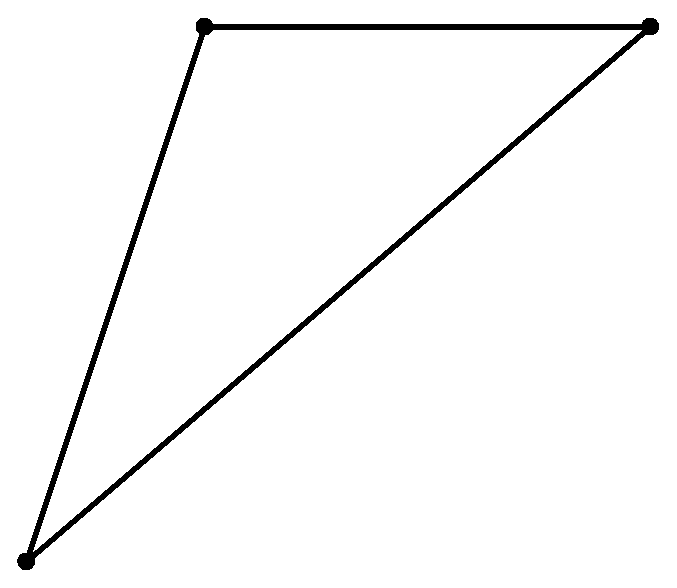
\includegraphics[width=0.35\textwidth]{sketch_triangle}}
        \vspace{0.2in}
        \subfloat[Reference Triangle.]
          {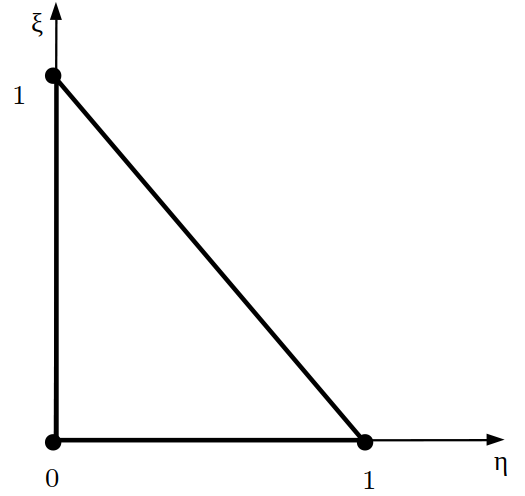
\includegraphics[width=0.35\textwidth]{Tref}}
        \caption{Description of Triangle Elements.}
        \label{fig:triangle_elements}
      \end{figure}

      It is difficult to analytically calculate the desired integral quantities
      for an arbitrary triangle. Instead, a simplified reference element is
      created and quantities are calculated for the reference element and then
      translated to the arbitrary element using a Jacobian.  The reference
      triangle $T_{ref}$ is located in $\xi \in [0,1]$ and $\eta \in [0,1-\xi]$.
      General and reference triangles are shown in \fref{fig:triangle_elements}.
      The basis functions are zero outside of the reference triangle. Within
      the reference triangle, basis functions for the are provided in the
      natural coordinates of $T_{ref}$.
      \begin{align}
        \basis_i(\xi,\eta) &= 0 \quad \forall \; (\xi,\eta) \notin T_{ref} \\
        \basis_1(\xi,\eta) &= \xi \\
        \basis_2(\xi,\eta) &= \eta \\
        \basis_3(\xi,\eta) &= 1-\xi-\eta
      \end{align}
      
      For linear triangles, simple expressions for the integral quantities for
      an arbitrary triangle can be derived \cite{textbookwhite}. The expression
      for the line integral for the arbitrary element can also be derived
      \cite{computerLab}. For a general triangle with corners $( x_i,y_i )$ with
      $i=1,2,3$
      \begin{align}
        \int_{\Omega_e} \grad \basis_i(\vr) \cdot \grad \basis_j(\vr) 
          \;d\vr &= \frac{1}{4 A_e}
          ((x_{i+1}-x_{i+2})(x_{j+1}-x_{j+2}) + 
          (y_{i+1}-y_{i+2})(y_{j+1}-y_{j+2})), \\
        \int_{\Omega_e} \basis_i(\vr) \basis_j(\vr) \;d\vr &= 
          \frac{A_e}{12} (1+\delta_{ij}), \\
        \int_{\Omega_e} \basis_i(\vr) \;d\vr &= \frac{A_e}{3}, \\
        \int_{\partial \Omega_e} \basis_i(\vr) \basis_j(\vr) \;ds &=
          \frac{L_e}{6}(1+\delta_{ij}), 
      \end{align}
      where $A_e$ is the area of the triangular element, $L_e$ is the length of 
      the edge between node $i$ and node $j$, and $\delta_{ij}$ is the Kronecker
      delta.
      The Kronecker delta is defined as
      \begin{equation} \label{eq:kroneker_delta}
        \delta_{ij} =
        \begin{cases}
          0 & \text{if } i \ne j, \\
          1 & \text{if } i = j.
        \end{cases}
      \end{equation}
      The area of a triangle in three dimensions is calculated for a triangle
      with corner coordinates $\vc_i = (x_i, y_i, z_i)$ with $i=1,2,3$.
      That is, $\vc_i$ is the coordinates of corner $i$. Calculation of the area
      of a general triangle is then given by the vector operations
      \begin{align}
        \va &= \vc_2 - \vc_1, \\
        \vb &= \vc_3 - \vc_1, \\
        A_e &= \half \lvert \va \times \vc \rvert, \\
        \label{eq:area_triangle}
        A_e &= \half \sqrt{ (a_2 b_3 - a_3 b_2)^2 + (a_3 b_1 - a_1 b_3)^2 +
          (a_1 b_2 - a_2 b_1)^2},
      \end{align}
      where $a_i$ is the $i^{th}$ component of vector $\va$ and $b_i$ is the
      $i^{th}$ component of vector $\vb$.  For higher order triangular elements
      (e.g. quadratic or cubic elements), it may be necessary to employ a
      quadrature to calculate the necessary integral quantities.

    \subsubsection{Linear Wedges}
      A wedge element is a pentahedron with six corner nodes, and is sometimes
      referred to as a triangular prism. A simple example of a wedge is an
      extruded triangle. However, unlike an extruded triangle, the exact 
      geometric relation of corner nodes in a wedge is not fixed and the nodes 
      are free to expand and distort. An example of typical and distorted
      wedge elements are shown in \fref{fig:sketch_wedge}. These elements are
      unique because there are two different types of faces. Three faces are
      quadrilateral and two are triangular. 

      \begin{figure}
        \centering
        \subfloat[General Wedge Element.]
          {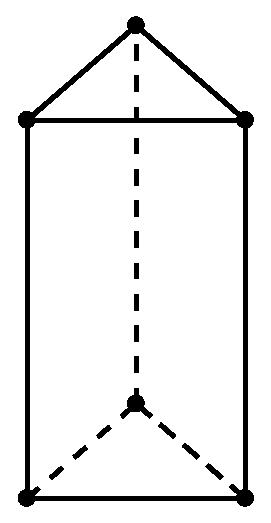
\includegraphics[width=0.2\textwidth]{wedge_sketch}}
        \vspace{0.5in}
        \subfloat[Distorted Wedge Element.]
          {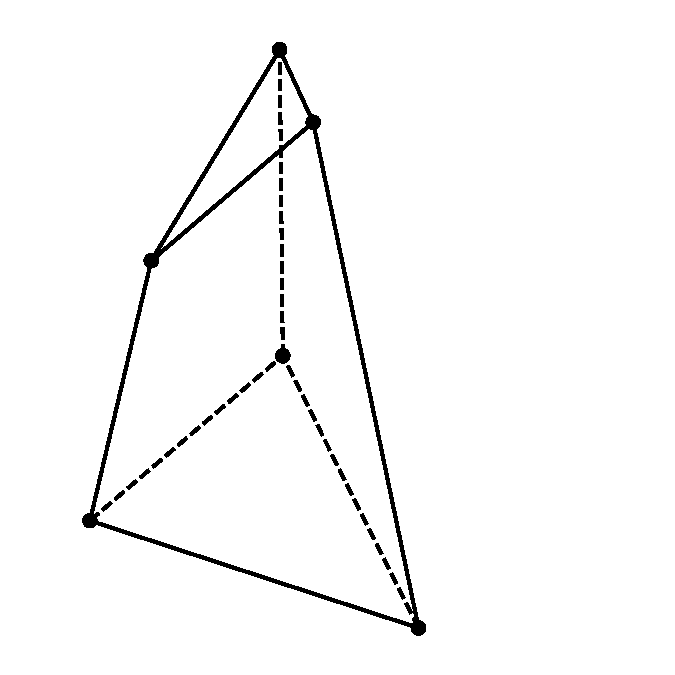
\includegraphics[width=0.2\textwidth]{wedge_stretch}}
        \caption{Description of Wedge Elements.}
        \label{fig:sketch_wedge}
      \end{figure}

      Fast reactors typically have hexagonal-z geometry so wedge elements are a 
      natural choice for this coordinate system. Reactor geometries are also 
      typically described in lattices so the wedge element allows for easily 
      ``stacking'' lattices on top of each other.

      \begin{figure}
        \centering
        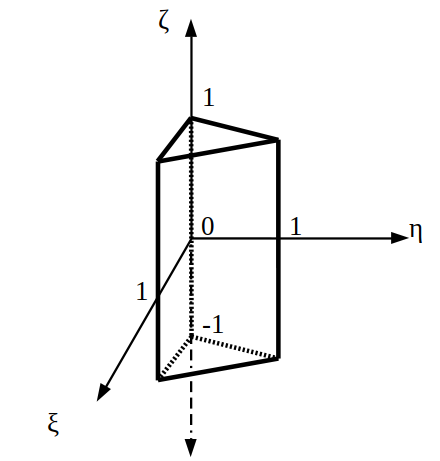
\includegraphics[width=0.3\textwidth]{Wref}
        \caption{Description of Reference Wedge.}
        \label{fig:Wref}
      \end{figure}

      The reference wedge $W_{ref}$ is located in 
      $\xi \in [0,1]$, $\eta \in [0,1-\xi]$, and $\zeta \in [-1,1]$. The
      coordinate system of the reference wedge is shown in \fref{fig:Wref}. The
      basis functions are zero outside of the reference wedge and are 
      provided within the reference wedge.
      \begin{align}
        \basis_i(\xi,\eta,\zeta) &= 0 \quad \forall \; (\xi,\eta,\zeta)
          \notin W_{ref} \\
        \basis_1(\xi,\eta,\zeta) &= \half (1-\zeta)(1-\xi-\eta) \\
        \basis_2(\xi,\eta,\zeta) &= \half (1-\zeta)\xi \\
        \basis_3(\xi,\eta,\zeta) &= \half (1-\zeta)\eta \\
        \basis_4(\xi,\eta,\zeta) &= \half (1+\zeta)(1-\xi-\eta) \\
        \basis_5(\xi,\eta,\zeta) &= \half (1+\zeta)\xi \\
        \basis_6(\xi,\eta,\zeta) &= \half (1+\zeta)\eta 
      \end{align}

      The integrals of the basis function over the element are given in
      \eref{eq:bigmat} through \eref{eq:wedge_surface_integral}. The values
      presented herein are not found in literature and have been calculated by
      the author. For a general wedge, the integral quantities are
      \begin{align}
        \label{eq:bigmat}
        \int_{\Omega_e} \basis_i(\vr) \basis_j(\vr) \;d\vr &= 
          \frac{V_e}{144}
          \begin{pmatrix}
            4 & 2 & 2 & 2 & 1 & 1 \\
            2 & 4 & 2 & 1 & 2 & 1 \\
            2 & 2 & 4 & 1 & 1 & 2 \\
            2 & 1 & 1 & 4 & 2 & 2 \\
            1 & 2 & 1 & 2 & 4 & 2 \\
            1 & 1 & 2 & 2 & 2 & 4 
          \end{pmatrix}, \\
        \int_{\Omega_e} \basis_i(\vr) \;d\vr &= \frac{V_e}{12}, \\
        \label{eq:wedge_surface_integral}
        \int_{\partial \Omega_e} \basis_i(\vr) 
          \basis_j(\vr) \;ds &= 
          \begin{cases}
            \frac{A_{\triangle}}{12}(1+\delta_{ij}) & 
              \text{if triangular surface,} \\
            \frac{A_{\Box}}{36}(1+\delta_{ij})(1-\half \delta_{i,(5-j)}) &
              \text{if quadrilateral surface,}
          \end{cases}
      \end{align}
      where $V_e$ is the volume of the element, $A_{\triangle}$ is the area of 
      the triangular surface, and $A_{\Box}$ is the area of the quadrilateral
      surface.  The matrix in \eref{eq:bigmat} is indexed $\mathbf{M}_{ij}$ and
      is presented as a matrix because of its irregular form. Notice the
      integral containing the gradient operator has been omitted because it is
      computed using a quadrature. If it could be computed analytically, it
      would be less computationally efficient than using a quadrature.
      
      $A_{\triangle}$ is computed according to \eref{eq:area_triangle} and
      $A_{\Box}$ is computed as the sum of the area of two triangles, employing
      the same formula. For a simple extruded triangle, the volume calculation 
      is straightforward and is the product of triangular area and linear 
      height. However, allowing the nodes to move with respect to each other 
      makes the volume of the element difficult to calculate. Therefore, the 
      Jacobian is used to calculate $V_e$. For more detail, see 
      \sref{sec:quadratures}, especially \tref{tab:jacobi}.

  \subsection{Quadratures}
    \label{sec:quadratures}
    Quadratures are sets of coordinates and weights which are used to
    approximate an integral.  For a given set of weights, $\{w_i\}$, and a set
    of coordinates, $\{\vx_i\}$, an integral can be represented as the sum
    \begin{equation}
      \label{eq:quadrature}
      \int_{\Omega} f(\vx) \;d\Omega \approx \sum_{i=1}^{N} f(\vx_i) \, w_i 
    \end{equation}
    where $\Omega$ is an arbitrary domain described by $\{\vx_i\}$.  A
    quadrature, such as the one in \eref{eq:quadrature}, can be designed to
    exactly integrate a polynomial of order $n$. It is not necessarily true that
    the number of quadrature points, $N$, will equal the order of the polynomial
    exactly integrated, $n$. Generally, $n \ne N$.
    
    For one-dimensional integrals, the Gaussian quadrature is common and the most compact quadrature. The Gaussian quadrature exactly integrates a 
    polynomial of order $n$ using exactly $N=n$ points. For this quadrature, the
    number of points in the quadrature is the same as the order of the
    quadrature and $n=N$.
    
    Two-dimensional and three-dimensional quadratures are necessary for the 
    \gls{fem}. Triangular quadratures are not as simple to derive
    as line quadratures and the number of points need not equal the order of the
    polynomial integrated. The triangular quadrature as implemented here is 
    symmetric and open. That is, there are no points on the boundary of the 
    triangle \cite{triangleQuadrature}. Any triangular quadrature will suffice
    that exactly integrates polynomials of a given order. There is no fixed
    relationship between $n$ and $N$ and for this quadrature, $n \ne N$.
    
    Quadrilateral quadrature sets are simply tensor products of two line 
    Gaussian quadratures. For an order $n$ polynomial, now $N^2=n$ points are 
    required. 
    
    Wedge quadrature sets are simply tensor products of a line Gaussian 
    quadrature and a triangular quadrature. Again, there is no fixed
    relationship between $n$ and $N$.
    
    Though only linear functions are used here, basis functions are generally
    polynomials of first, second, or third order; that is, linear, quadratic, or
    cubic functions. The quadratures described are capable of exactly
    integrating polynomial functions of given order so there exists a quadrature
    order that will exactly integrate the finite element quantities to numeric
    precision. The table of the order required for exact integration are
    provided in \tref{tab:quadrature_orders}.

    \begin{table}
      \begin{center}
        \caption{Quadrature Orders for \glsentryshort{fem} Quantities.}
        \label{tab:quadrature_orders}
        \begin{threeparttable}
          \begin{tabular*}{0.8\textwidth}{@{\extracolsep{\fill}}lccc}
            \toprule
            Quantity & Linear & Quadratic & Cubic \\
            \midrule
            $\int_{\Omega} \basis_i(\vr) \;d\Omega$ & 1 & 2 & 4
              \tnote{$\dagger$} \\
            $\int_{\Omega} \basis_i(\vr) \basis_j(\vr) \;d\Omega$ &
              2 & 4 & 6 \\
            $\int_{\Omega} \grad \basis_i(\vr) \cdot \grad \basis_j(\vr) 
              \;d\Omega$ & 2 & 3 & 5 \\
            \bottomrule
          \end{tabular*}
          \begin{tablenotes}
            \item[$\dagger$] A third-order quadrature would be exact but the 
              triangular quadrature would have negative weights so a fourth 
              order quadrature is selected.
          \end{tablenotes}
        \end{threeparttable}
      \end{center}
    \end{table}
    
    All of the quadratures described here are tabulated for a reference element
    be it a line, triangle, quadrilateral, or wedge. Integration in the 
    \gls{fem} is performed on an arbitrary element in space. Therefore, it is 
    necessary to perform a coordinate transform when using a quadrature set.
    % get VERY explicit here so someone else can actually solve the problem...
    Integration with transformed coordinates from domain $\Omega$ to the
    reference domain $\Omega_{ref}$ can be written
    \begin{equation}
      \int_{\Omega} f(\vx) \;d\Omega = 
        \int_{\Omega_{ref}} f(\vx) \lvert \mj \rvert \;d\Omega_{ref} \approx
        \sum_{i=1}^{N} w_i f(\vx_i) \lvert \mj_i \rvert
    \end{equation}
    where $\mj$ is the Jacobian matrix, $\mj_i$ is the Jacobian matrix at 
    quadrature coordinate $\vx_i$, and $\lvert \cdot \rvert$ represents
    the matrix determinant. Notationally, $J=\lvert \mj \rvert$ and is termed
    the Jacobi.

    Isoparametric elements are elements in which shape functions can be used to
    relate global coordinates, $(x,y,z)$, to local coordinates
    $(\xi,\zeta,\eta)$. Generally, non-curved elements are isoparametric. For
    isoparametric elements, such as triangles and wedges, the Jacobi is constant
    over the element and can be pre-calculated. Pre-calculating the Jacobi
    avoids populating and evaluating the determinant of a matrix for each
    integration point. For the elements of concern, these values are presented
    in \tref{tab:jacobi} \cite{textbookcolorado}.

    \begin{table}
      \caption{Jacobi for Selected Elements.}
      \label{tab:jacobi}
      \begin{center}
        \begin{tabular}{ll}
          \toprule
          Element & $J$ \\
          \midrule
          Triangle      & $A_e$ \\
          Quadrilateral & $\frac{1}{4} A_e$ \\
          Wedge         & $\half V_e$ \\
          \bottomrule
        \end{tabular}
      \end{center}
    \end{table}

    For the general element, the Jacobian matrix, $\mj_i$, is calculated at each
    point of the quadrature $(\xi_i,\zeta_i,\eta_i)$ as described in
    \eref{eq:calcJacobian}.
    \begin{equation}
      \label{eq:calcJacobian}
      \mj_i = 
      \begin{pmatrix}
        \sum_{k=1}^{N_P} \left. \frac{\partial \basis_k}{\partial \xi}
          \right|_{(\xi_i,\zeta_i,\eta_i)} x_k   \; &
        \sum_{k=1}^{N_P} \left. \frac{\partial \basis_k}{\partial \zeta}
          \right|_{(\xi_i,\zeta_i,\eta_i)} x_k   \; &
        \sum_{k=1}^{N_P} \left. \frac{\partial \basis_k}{\partial \eta} 
          \right|_{(\xi_i,\zeta_i,\eta_i)} x_k   \\
        \sum_{k=1}^{N_P} \left. \frac{\partial \basis_k}{\partial \xi}
          \right|_{(\xi_i,\zeta_i,\eta_i)} y_k   \; &
        \sum_{k=1}^{N_P} \left. \frac{\partial \basis_k}{\partial \zeta} 
          \right|_{(\xi_i,\zeta_i,\eta_i)} y_k   \; &
        \sum_{k=1}^{N_P} \left. \frac{\partial \basis_k}{\partial \eta} 
          \right|_{(\xi_i,\zeta_i,\eta_i)} y_k   \\
        \sum_{k=1}^{N_P} \left. \frac{\partial \basis_k}{\partial \xi}
          \right|_{(\xi_i,\zeta_i,\eta_i)} z_k   \; &
        \sum_{k=1}^{N_P} \left. \frac{\partial \basis_k}{\partial \zeta} 
          \right|_{(\xi_i,\zeta_i,\eta_i)} z_k   \; &
        \sum_{k=1}^{N_P} \left. \frac{\partial \basis_k}{\partial \eta} 
          \right|_{(\xi_i,\zeta_i,\eta_i)} z_k   
      \end{pmatrix}
    \end{equation}
    In \eref{eq:calcJacobian}, $N_P$ is the number of points in the element, 
    $\basis_k(\vr)$ is the basis function centered at the $k^{th}$ corner, and 
    for corner coordinates $(x_k,y_k,z_k)$ for $k = 1,2,\ldots,N_P$.

    With the Jacobian populated as \eref{eq:calcJacobian}, $J=\lvert\mj\rvert$
    is simply the matrix determinant. For the quadrature integration of 
    derivative quantities as necessary in the \gls{fem}, the derivatives must 
    also be translated from the reference element to the spatial element. This 
    is performed according to \algorithmref{algorithm:deriv_int}. The notation 
    is dense as the method requires two sets of coordinates. First, the 
    coordinate in the reference element $(\xi,\zeta,\eta)$ and second, the 
    coordinate in Cartesian space $(x,y,z)$.

    The vector $\vd_{i,\,(\xi,\zeta,\eta)}$ is the gradient vector for
    $\basis_i$ with respect to the reference coordinates $(\xi,\zeta,\eta)$.
    \begin{equation}
      \vd_{i\,(\xi,\zeta,\eta)} = \grad_{(\xi,\zeta,\eta)} N_i(\vr) 
    \end{equation}
    Vector $\vd_{i,\,(x,y,z)}$ is the gradient vector for $\basis_i$ with
    respect to the Cartesian coordinates $(x,y,z)$. 
    \begin{equation}
      \vd_{i,\,(x,y,z)} = \grad_{(x,y,z)} N_i(\vr)
    \end{equation}
    In \algorithmref{algorithm:deriv_int}, the quadrature has points $\{\vx_p\}$ 
    and weights $\{w_p\}$ for $p = 1,2,\ldots,N$ and the value of the integral,
    $v$, is represented by \eref{eq:deriv_integral}.
    \begin{equation}
      \label{eq:deriv_integral}
      v = \int_{\Omega_e} \grad_{(x,y,z)} \basis_i(\vr) \cdot 
        \grad_{(x,y,z)} \basis_j(\vr) \; d\Omega_e
    \end{equation}

    \begin{algorithm}
      \caption{Integral of Derivative with Jacobian Method.}
      \label{algorithm:deriv_int}
      \begin{algorithmic}[1]
        \State $v=0$
        \For{$p=1,N_P$}
          \State Calculate the Jacobian $\mj$ as in \eref{eq:calcJacobian}.
          \State Calculate the vector $\vd_{i,\,(\xi,\zeta,\eta)}$ at quadrature
            point $\vx_p$.
          \State Calculate the vector $\vd_{j,\,(\xi,\zeta,\eta)}$ at quadrature
            point $\vx_p$.
          \State Invert and store the Jacobian $\mj^{-1}$.
          \State Calculate the vector $\vd_{i,\,(x,y,z)} =
            \vd_{i,\,(\xi,\zeta,\eta)} \mj^{-1}$.
          \State Calculate the vector $\vd_{j,\,(x,y,z)} =
            \vd_{j,\,(\xi,\zeta,\eta)} \mj^{-1}$.
          \State $v = v + \left(\vd_{i,\,(x,y,z)}^{T} \vd_{j,\,(x,y,z)}\right)
            \, w_p \, \lvert \mj \rvert$
        \EndFor
      \end{algorithmic}
    \end{algorithm}

\section{Power Iterations}
  \label{sec:power_iterations}
  The \gls{fem} is used to solve a fixed source problem for a given source
  distribution $q_g(\vr)$. However, for multigroup problems with a fission
  source, the problem is an eigenvalue problem and the source is not known.
  For eigenvalue problems, the problem does not have a fixed source and the
  system has many solutions. The method of Power Iterations allows eigenvalue
  problems to be solved iteratively for the fundamental eigenvalue and
  eigenvector.

  \subsection{Convergence of Power Iteration Method}
    Noting the \gls{fem} equations can be written as matrix form
    \eref{eq:matrix_notation}, the discretized multigroup neutron diffusion 
    equation can be rewritten as shown by \textcite{gehinThesis} as
    \begin{equation}
      \label{eq:gehin_notation}
      \mb(\vPhi,\keff) \vPhi = \frac{1}{\keff} \mm \vPhi
    \end{equation}
    where $\vPhi$ is the vector of the flux containing all energy groups, matrix 
    $\mb$ contains the diffusion, removal, and all scattering terms, and $\mm$ 
    includes all fission generation and operates on $\vPhi$ and $\keff$. $\mb$
    is an S-matrix and its inverse, $\mb^{-1}$, exists and has all positive 
    elements \cite{nakamura}. Therefore, \eref{eq:gehin_notation} can be 
    rewritten as
    \begin{equation}
      \label{eq:gehin_solution}
      \vPhi = \frac{1}{\keff} \mr \vPhi
    \end{equation}
    where
    \begin{equation}
      \label{eq:gehin_r}
      \mr = \mb^{-1} \mm.
    \end{equation}
    Matrix $\mm$ is non-symmetric and is non-negative and $\mb$ is an S-matrix;
    therefore, $\mr$ is a non-symmetric, non-negative matrix.

    In the solution of \eref{eq:multigroup_diffusion}, the largest eigenvalue,
    $\keff$, is desired along with its associated eigenvalue, $\phi_g$. The
    solution can be found using the method of power iterations which can be
    written as 
    \begin{align}
      \label{eq:power_iteration_phi}
      \vPhi^{(s+1)} &= \frac{1}{\keff^{(s)}} \mr \vPhi^{(s)}, \\
      \label{eq:power_iteration_eigenvalue}
      \keff^{(s+1)} &= \keff^{(s)} \frac{\vw^{T} \vPhi^{(s+1)}}
        {\vw^{T} \vPhi^{(s)}}, \qquad s = 1,2,\ldots,\infty,
    \end{align}
    where $s$ is the iteration counter, $\vw$ is a weighting vector and 
    $\vw^{T} \vPhi$ is the vector inner-product. According to the 
    Perron-Frobenius theorem, a matrix with the properties of $\mr$ has a 
    unique, positive eigenvalue, greater in magnitude than the modulus of all 
    other eigenvalues of the matrix. The weighting vector $\vw$ is arbitrary 
    but does affect convergence rate. For this work,
    $\vw = \{\nu \Sigma_f\}$ such that the inner product 
    $\{\nu \Sigma_f\}^T \vPhi$ represents the summation of the fission neutron
    production rate throughout all energy groups and all elements. 
    
    It can then be shown in that the method of power iterations described in 
    \eref{eq:power_iteration_phi} and \eref{eq:power_iteration_eigenvalue}
    converges to the largest eigenvalue, $\keff$, and unique positive 
    eigenvector $\vPhi$ \cite{nakamura}. For notation and enumeration, allow the 
    eigenvalue to be rewritten as
    \begin{equation}
      \label{eq:mu}
      \mu = \frac{1}{\keff}.
    \end{equation}
    The eigenvectors $\vu_n$ and
    corresponding eigenvalues $\mu_n$ of $\mr$ are defined by
    \begin{equation}
      \label{eq:eigen_definition}
      \vu_n = \mu_n \, \mr \, \vu_n.
    \end{equation}
    It may be proved that all eigenvalues $\mu$ are real, positive, and 
    distinct. The eigenvalues are then numbered in the sequence
    \begin{equation}
      \label{eq:eigen_order}
      \mu_0 < \mu_1 < \mu_2 < \cdots < \mu_N
    \end{equation}
    where $N$ is the rank of the problem. The eigenvectors have the 
    orthogonality relations
    \begin{equation}
      \label{eq:eigen_orthogonality}
      \vu^T_n \vu_m = 0  \qquad \text{for } n \ne m
    \end{equation}
    where $\vu^T \vu$ is the vector inner-product. Assume eigenvectors are
    normalized such that
    \begin{equation}
      \label{eq:eigen_normalization}
      \vu_n^T \vu_n = 1 \qquad \text{for } n = 1, 2, \ldots, N.
    \end{equation}
    The initial vector $\vPhi^{(0)}$ may be expressed as a projection onto the
    eigenvectors using a linear superposition of eigenvectors of the form
    \begin{equation}
      \label{eq:eigen_projection}
      \vPhi^{(0)} = \sum_{n=1}^{N} c_n^{(0)} \vu_n
    \end{equation}
    where $c_n^{(0)}$ is a coefficient given by the orthogonality relationship
    from \eref{eq:eigen_orthogonality} such that
    \begin{equation}
      \label{eq:eigen_cn}
      c_n^{(0)} = \vu_n^T \vPhi^{(0)}.
    \end{equation}
    Using this eigenmode projection, \eref{eq:power_iteration_phi} can be
    rewritten as 
    \begin{equation}
      \label{eq:phi_expand_begin}
      \vPhi^{(s+1)} = \mu^{(s)} \, \mu^{(s-1)} \, \mu^{(s-2)} \, 
        \ldots \, \mu^{(0)} \, \mr \phi^{(0)}.
    \end{equation}
    Then, \eref{eq:eigen_projection} can be inserted into
    \eref{eq:phi_expand_begin}.
    \begin{align}
      \vPhi^{(s+1)} &= \mu^{(s)} \, \mu^{(s-1)} \, \ldots \, 
        \mu^{(0)} \sum_{n=1}^N c_n^{(0)} \, \mr \, \vu_n \\
      &= \left( \prod_{p=0}^{s} \mu^{(p)} \right) \sum_{n=1}^N c_n^{(0)} \, 
        \mr \, \vu_n
    \end{align}
    Recalling the relationship \eref{eq:eigen_projection}.
    \begin{equation}
      \label{eq:phi_expand_above}
      \vPhi^{(s+1)} = \left( \prod_{p=0}^s \mu^{(p)} \right) 
        \sum_{n=1}^N c_n^{(0)} \frac{1}{\mu_n^{(s+1)}} \vu_n
    \end{equation}
    \eref{eq:phi_expand_above} can be rewritten by dividing and multiplying by
    $\mu_0$ and dividing and multiplying by $c_0$.
    \begin{align}
      \vPhi^{(s+1)} &= \left( \prod_{p=0}^s \frac{\mu^{(p)}}{\mu_0} 
        \right) c_0 \left( \vu_0 \sum_n^N \frac{c_n^{(0)}}{c_0^{(0)}}
        \frac{\mu_0}{\mu_n^{(s+1)}} \vu_n \right) \\
      \label{eq:eigen_phi_converge}
      \vPhi^{(s+1)} &\approx \text{const.} \cdot \left( 
        \vu_0 \sum_n^N \frac{c_n^{(0)}}{c_0^{(0)}}
        \frac{\mu_0}{\mu_n^{(s+1)}} \vu_n \right)
    \end{align}
    The ordering of unique eigenvalues required by \eref{eq:eigen_order} 
    requires $\mu_0 / \mu_n < 1$ and the problem is convergent. The 
    convergence rate is determined by the dominance ratio, $d$, where
    \begin{equation}
      \label{eq:dominance_ratio}
      d \equiv \max_{n=1,2,\ldots,N} \frac{\mu_0}{\mu_n} =
        \frac{\mu_0}{\mu_1}
    \end{equation}
    and it can be seen that for problems with small dominance ratio, the power
    iteration method will converge more quickly. As the dominance ratio
    approaches unity, $d \rightarrow 1$, the power iteration method will be
    slower to converge. Convergence criteria are then specified as an absolute 
    tolerance in the sense of the eigenvalue
    \begin{equation}
      \label{eq:eigenvalue_tol}
      \epsilon_{\mu} > | \mu^{(s+1)} - \mu^{(s)} |
    \end{equation}
    and as a relative tolerance in the sense of the eigenvector
    \begin{equation}
      \label{eq:eigenvector_tol}
      \epsilon_{\vPhi} > \max_i \left| \frac{\vPhi_i^{(s+1)} - \vPhi_i^{(s)}}
        {\vPhi_i^{(s)}}\right| .
    \end{equation}

    It is important to note that all of the analysis in this section assumed the
    matrix $\mr$ does not change between iterations. For simple multigroup
    criticality calculations, this assumption is correct. However, in
    multiphysics nuclear power reactor simulations, the cross sections of the 
    problem may be considered functions of material temperature or may have some
    variable number density. For these problems, the matrix $\mr$ is necessarily
    updated between power iterations in a nonlinear manner. For nonlinear power
    iteration updates, convergence is no longer guaranteed. The argument for
    convergence with nonlinear power iterations in this implementation falls
    back to the stability of the physical system.
    
  \subsection{Calculation of Source with Power Iterations}
  \label{sec:calculation_of_source_with_power_iterations}
    The multigroup neutron diffusion equation \eref{eq:multigroup_source} can be
    written with the source term $q_g(\vr)$ expanded into its component parts.
    \begin{equation} \label{eq:multigroup_source_expand}
      -\grad \cdot (D_g(\vr) \grad \phi_g^{(s)}(\vr)) + \Sigma_{r,g}(\vr)
      \phi_g^{(s)}(\vr) = q_{fiss,g}(\vr) + q_{up,g}(\vr) + q_{down,g}(\vr)
    \end{equation}
    Recall from the definitions of the source components that their calculation
    requires the flux $\phi_g(\vr)$. The source components each require
    different energy groups of the flux distribution to be known. The fission
    component $q_{fiss,g}(\vr)$ requires all groups. The up-scatter component
    $q_{up,g}(\vr)$ requires lower energy groups (i.e. $g' > g$). The
    down-scatter component $q_{down,g}(\vr)$ requires higher energy groups (i.e.
    $g' < g$). Based on these requirements, these source components can be
    calculated based on different iterations within the power iteration method.
    This is described in \algorithmref{algorithm:general}.
    \eref{eq:multigroup_source_expand} is then more explicitly written.
    \begin{equation} 
      \label{eq:multigroup_power_iterations}
      -\grad \cdot (D_g(\vr) \grad \phi_g^{(s+1)}(\vr)) + \Sigma_{r,g}(\vr)
      \phi_g^{(s+1)}(\vr) = q_{fiss,g}^{(s)}(\vr) + q_{up,g}^{(s)}(\vr) +
      q_{down,g}^{(s+1)}(\vr)
    \end{equation}

\section{Implementation}
  A \gls{fem} neutron diffusion solution has been developed using 
  the above formulae. The program begins by reading a geometry description 
  specified in a plain text VTK file \cite{vtk}. The VTK format is chosen 
  because it is a standard that can be used with visualization tools such as 
  ParaView \cite{ParaView} and VisIt \cite{VisIt}. Additionally, open-source C 
  and Python packages exist for easy manipulation of the format. Cross sections
  are specified in either a plain text user format or the ISOTXS format as 
  common to fast reactor applications and the multigroup cross section generator
  \mcc \cite{mcc}. The multigroup neutron diffusion equation is solved according
  to \eref{eq:multigroup_source}. The resulting effective neutron multiplication 
  factor, $\keff$, is written to an output file. The multigroup neutron flux is
  written to a different results VTK file for easy visualization. In a
  multiphysics simulation, material temperatures and thermal expansion
  dimensions are also written to the results VTK.

  \subsection{Algorithm}
    The algorithm for the solution to the diffusion equation is similar to most
    implementations of the power iteration method to solve the multigroup
    neutron diffusion equation. The algorithm itself is presented in 
    \algorithmref{algorithm:general}. The steps unique to the \gls{fem} are 
    steps \ref{state:fem_matrix} and \ref{state:fem_vector}. These require the 
    quantities previously derived and form the linear system described by the 
    \gls{fem}. 

    In step \ref{state:rcm} the matrix is reordered. Mathematically this has no
    effect on the result as the linear system represented is equivalent. This 
    choice to reorder the system is made to improve computational efficiency. 
    Indexing nodes that are physically proximate with proximate indices causes 
    rows in the finite element matrix, $\ma_g$, to be closely coupled to nearby
    rows. In a general unstructured and unordered mesh, rows may be coupled to 
    other random rows in the matrix. This step of reordering the matrix $\ma_g$ 
    seeks to decrease the bandwidth of the matrix and encourage cache hits when
    accessing coupled values in the linear system. The ordering chosen is the
    \gls{rcm} method and common to sparse linear systems
    \cite{rcm}. An example of the bandwidth reduction provided by the \gls{rcm}
    method is shown in \fref{fig:sparsity_pattern}. The plots show the
    sparsity pattern of the matrix before and after reordering. After
    reordering, the matrix bandwidth is reduced from 2,326 to 81.

    \begin{figure}
      \centering
      \subfloat{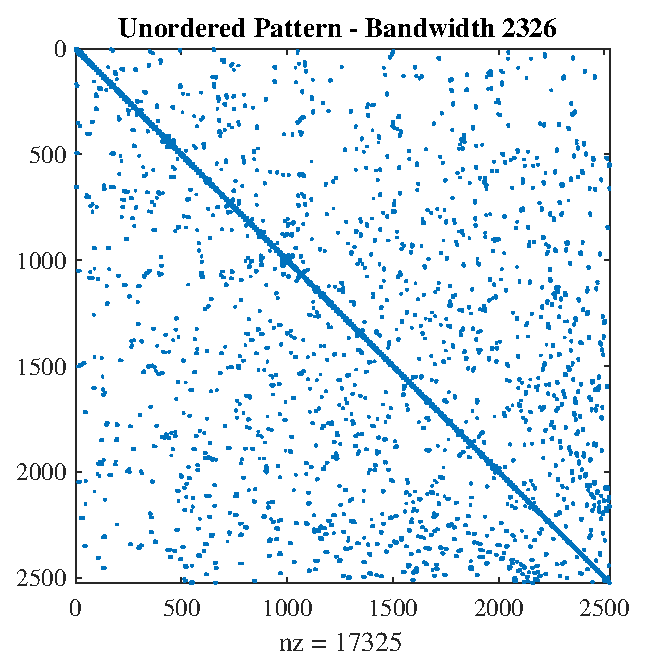
\includegraphics[width=0.4\textwidth]{uno_pattern}}
      \hspace{0.1in}
      \subfloat{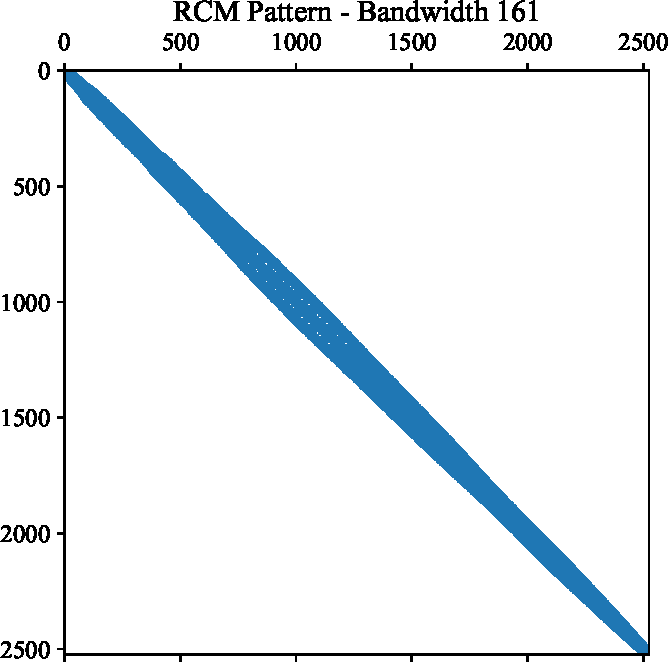
\includegraphics[width=0.4\textwidth]{rcm_pattern}}
      \caption{Demonstration of \glsentryshort{rcm} Matrix Ordering.}
      \label{fig:sparsity_pattern}
    \end{figure}
    
    \begin{algorithm}
      \caption{General Iteration Scheme}
      \label{algorithm:general}
      \begin{algorithmic}[1]
      \State Read mesh from VTK.
      \State Initialize $\phiavg_g^{(0)}$.
      \State Order the nodes of the mesh into \gls{rcm} order.
        \label{state:rcm}
      \State Calculate $\Sigma_{s,g'\rightarrow g}$, $\Sigma_{r,g}$, and 
        $\nu \Sigma_{f,g}$ for each element.
      \State Calculate finite element matrix $\ma_g$ for each group. Store this. 
        \label{state:fem_matrix}
      \While{Power Iteration}
        \State Update the iteration counter. $s=s+1$
        \State Update $q_{fiss,g}$ and $q_{up,g}$ for all groups from previous 
          data $\phiavg^{(s-1)}$.
        \State Update $\widetilde{\chi_g}$ in each element using previous data.
          \label{state:chi_collapse}
        \For{$g=1,G$}
          \State Update $q_{down,g}$ from current data $\phiavg_g^{(s)}$
          \State Calculate total source in each element.
          \State Update finite element Vector $\vf_g$ with new source.
            \label{state:fem_vector}
          \State Solve $\ma_g \vu_g = \vf_g$ using an iterative technique (See
            \sref{sec:linear_system_solution}).
          \State Parse $\vu_g$ for $\phi_g$ solution on nodes.
          \State Calculate element-average $\phiavg_g$.
        \EndFor
        \State Update $\keff$.
        \State Check convergence.
        \State Perform non-linear update if necessary and update $\ma_g$. 
          \label{state:nonlinear}
      \EndWhile
      \end{algorithmic}
    \end{algorithm}

    Step \ref{state:nonlinear} in \algorithmref{algorithm:general} incorporates
    the possibility of non-linear updates into the power iteration method. This
    invalidates the proof of convergence from \sref{sec:power_iterations} but is
    performed to simulate thermal hydraulic and thermal expansion effects as
    described in \chref{ch:thermalHydraulics} and \chref{ch:thermalExpansion}
    respectively. This procedure is commonly used in practice and no convergence 
    problems have been observed. This update also requires recalculating the 
    finite element matrix, $\ma_g$, for each group.
    
    A benefit of this implementation is that the finite element vector $\vf_g$
    must be updated on each power iteration of the solution whereas the matrix
    $\ma_g$ is described entirely by geometry and the material cross sections.
    For this reason, in problems with no multiphysics simulations, $\ma_g$ can
    be generated once at the beginning of the problem and stored for the
    duration of the calculation.

    \FloatBarrier % make sure the algorithm is in the correct section

  \subsection{Memory and Storage}
    The finite element matrix, $\ma_g$, is large and sparse so a sparse storage 
    and sparse solution to the linear system are required. Many sparse matrix 
    implementations have been described and implemented in the past including
    triplet, reduced column, and reduced row storage \cite{sparseBLAS}.  For 
    this work a \twotable method is chosen which was uniquely developed. 
    \twotable storage is chosen for its simplicity and implementation with the 
    \gls{fem}. Future work may include a reduced row implementation but there 
    will be a trade-off between memory minimization and computational 
    efficiency.
    
    The \twotable method is composed of two separate matrices in memory. An
    integer index table, \texttt{IDX}, and an IEEE double precision value table
    \texttt{VAL}. Table \texttt{IDX} is is dimension $DOF \times D$ where $DOF$
    is the number of degrees of freedom of the linear system and $D$ is the
    maximum number of nodes that a node shares including itself. $D$ is the
    degree of the matrix plus one. This must be determined at the beginning of
    the problem based on the input geometry.  Table \texttt{VAL} is dimension
    $DOF \times D \times G$ where $G$ is the number of energy groups as the
    matrix $\ma_g$ is group dependent.
    
    \texttt{IDX} is initialized to -1 and \texttt{VAL} is initialized 
    to 0.0 such that an index of -1 corresponds to a null entry in the 
    matrix. \texttt{IDX} is then populated with a modified adjacency graph. 
    Values in \texttt{IDX} indicate the column in which the \texttt{VAL} entry
    occurs. An example unstructured mesh is given in \fref{fig:adjacency_graph}. 
    Then, for node 5, the table \texttt{IDX} may resemble \eref{eq:idx_example}.
    \begin{equation}
      \label{eq:idx_example}
      \texttt{IDX}(:,5) = (8, 200, 48, 96, 5 )
    \end{equation}

    \begin{figure}
      \centering
      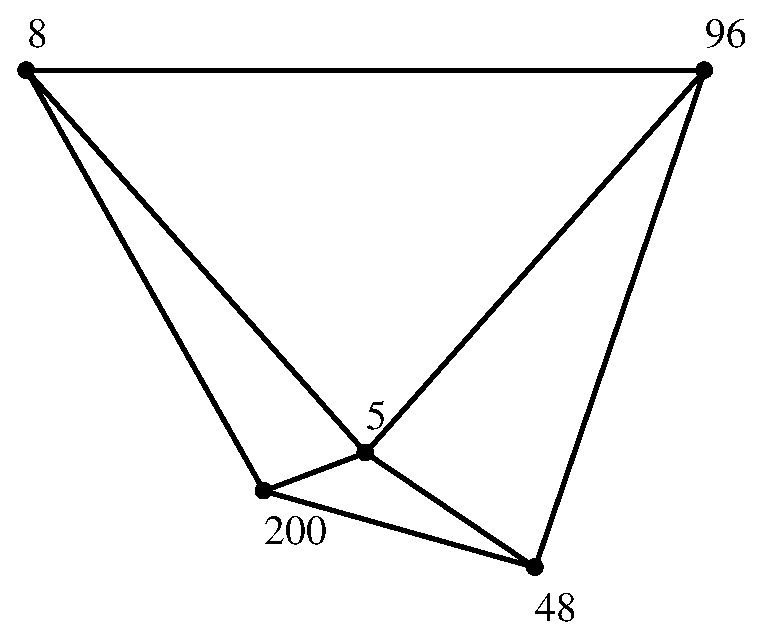
\includegraphics[width=0.5\textwidth]{adjacency_graph}
      \caption{Example Unstructured Mesh.}
      \label{fig:adjacency_graph}
    \end{figure}

    \eref{eq:idx_example} is only an example because the order of the nodes in 
    row 5 is arbitrary. Similarly, a numeric example is provided in 
    \eref{eq:idx_number} (note that the value ``3'' is arbitrary).
    \begin{equation}
      \label{eq:idx_number}
      \left.
      \begin{array}{c}
        \texttt{IDX}(7,3) = 8 \\
        \texttt{VAL}(7,3,g) = 12.1
      \end{array}
      \right\}
      \implies
      A_{7,8,g} = 12.1
    \end{equation}
    \eref{eq:idx_number} indicates that the value of matrix $\ma_g$ for group
    $g$ in the seventh row in the eighth column is 12.1. This will allow for 
    simple row operations and efficient matrix-vector multiplication which will
    be necessary in the solution of the linear system.

  \subsection{Boundary Conditions}
    \label{sec:boundary_conditions}
    Boundary conditions merit brief consideration. There are many ways to 
    implement boundary conditions and all result in mathematically the same 
    solution. The choices made for this work are presented below. Mirror 
    boundary conditions require $\grad \phi_g(\vr) = 0$ for 
    $\vr \in \partial \Omega$. These are termed ``natural'' boundary
    conditions because the finite element matrix, $\ma_g$, requires no
    additional treatment and this condition is natural. In the albedo
    representation, this is equivalent to $\albedo = 0$.
    
    Albedo boundary conditions are treated with an additional contribution to 
    the finite element matrix, $\ma_g$. These contributions represent a line 
    integral in two dimensions and a surface integral in three dimensions. These
    values are found in \eref{eq:matrix_population} and the quantities are 
    expressed in \sref{sec:matrix_quantities} or by quadratures 
    \sref{sec:quadratures}.
    
    Zero-flux boundary conditions require $\phi_g(\vr) = 0$ for $\vr \in
    \partial \Omega$. These are treated by removing these entries from the
    finite element matrix, $\ma_g$. Entries are removed by using an index vector.
    In a problem with only mirror and albedo boundary conditions, each node
    corresponds to an index row/column of the matrix. With entries removed, node
    number and index number may not exactly agree. A vector \texttt{ID} is
    introduced to track node numbers and their location in the finite element
    matrix, $\ma_g$ \cite{textbookjohnson}. Nodes with non-zero flux boundary
    conditions are set to a sequential positive integer. Nodes with zero-flux
    boundary conditions are set to a negative integer (-1) and are omitted in
    the actual solution of the system. Other strategies have been proposed such
    as the penalty approach \cite{textbookhughes} and forcing the solution of
    the linear system \cite{textbookli}. This method is chosen because it
    decreases the degree of freedom of the linear system while encouraging a
    well conditioned matrix.  Now, the degree of freedom of the matrix is equal
    to the number of nodes with non-zero flux boundary conditions.
    Alternatively, zero-flux boundary conditions can be represented as $\albedo
    \rightarrow \infty$.
    
  \subsection{Linear System Solution}
    \label{sec:linear_system_solution}
    For a non-singular linear system $\ma_g \vu_g = \vf_g$, where $\ma_g$ is a 
    square matrix, there exists a unique solution. Many strategies have been 
    proposed to solve this system in an efficient manner. Options are restricted
    in this work because the solution must operate with a sparsely stored linear
    system and result in no fill-in. This immediately demands an iterative
    method. The linear system described by the \gls{fem} can then be exploited
    for its unique properties to select a favorable solution method.
    
    The finite element matrix $\ma_g$ for the problem described in
    \eref{eq:multigroup_source} is \gls{spd} if the multigroup equations are
    solved one group at a time as they are in this work. Note, the matrix will 
    not have this especially useful property if all the groups were instead
    solved simultaneously. The symmetry condition is straight-forward and is
    observed in the elemental matrix description \eref{eq:matrix_population}.
    Briefly, $\ma_g^T = \ma_g$ because the elements ${A_{i,j,g,e}=A_{j,i,g,e}}$.
    Positive definiteness is a particularly useful condition but is often
    difficult to prove. $\ma_g$ is sometimes diagonally dominant for
    conveniently ordered meshes composed certain elements but generally, the
    matrix is not diagonally dominant. 
    
    A matrix $\ma_h \in \realnn$ is positive definite if
    \begin{equation} \label{eq:positive_definite}
      \vx^{T} \ma_g \vx > 0 \qquad \forall \; \vx \in \realn, \; \vx \ne 0.
    \end{equation}
    Let $\vx = \{x_i\}$ for $i = 1,2,\ldots,N$. Then the vector-matrix and 
    matrix-vector products can be rewritten as summations \cite{textbookhughes}.
    \begin{equation}
      \vx^{T} \ma_g \vx = \sum_{i=1}^{N} \sum_{j=1}^{N} x_i A_{ij} x_j
    \end{equation}
    By the definition of $A_{i,j,g}$ in \eref{eq:matrix_population} and 
    \eref{eq:fem_notation}.
    \begin{equation}
      \vx^{T} \ma_g \vx = 
        \sum_{i=1}^{N} \sum_{j=1}^{N} x_i a_g(\basis_i,\basis_j) x_j
    \end{equation}
    Noting the property that $a_g(\cdot,\cdot)$ is a bilinear operator (i.e.
    linear in both arguments) \cite{textbookli}.
    \begin{equation}
      \vx^{T} \ma_g \vx =
        a_g \left( \sum_{i=1}^{N} x_i \basis_i, \sum_{j=1}^{N} x_j \basis_j 
        \right)
    \end{equation}
    By construction of the \gls{fem}, $w(\vr) = \sum_{i=1}^{N} x_i \basis_i$ 
    where $w(\vr)$ is a piecewise continuous polynomial of arbitrary order.
    \begin{equation}
      \vx^{T} \ma \vx = a_g \left(w(\vr),w(\vr)\right)
    \end{equation}
    $a(\cdot,\cdot)$ can be shown to form a norm $\|\cdot \|_a$
    \cite{textbookli} satisfying the positive definite condition
    \eref{eq:positive_definite}.
    \begin{equation}
      \vx^{T} \ma_g \vx > 0 \qquad \forall \vx \in \realn, \; \vx \ne 0
    \end{equation}
    
    A given matrix can be verified as positive definite by one of two methods.
    First, all eigenvalues of the matrix have positive real components. Second,
    the matrix has a Cholesky decomposition such that $\ma = \ml \, \ml^*$ where
    $\ml$ is a lower triangular matrix with positive diagonal entries and
    $\ml^*$ is the conjugate transpose of matrix $\ml$ \cite{textbookipsen}. For
    real valued matrices, the conjugate transpose is equivalent to the
    conventional transpose. Though an eigenvalue decompisition or a Cholesky
    factorization may be useful for debugging or numerical analysis purposes, 
    these operations are computationally expensive. Instead, this is verified 
    here for the general matrix and not tested during simulations.
    
    Conventional methods used to solve a linear system described by an \gls{spd}
    matrix include Gauss-Seidel iteration with \gls{sor} and the \gls{cg} Krylov 
    subspace method. \gls{sor} requires \textit{a priori} knowledge of the 
    optimized over-relaxation factor, $\omega_{opt}$, for optimal performance. 
    In practice, calculation of $\omega_{opt}$ is performed analytically for 
    contrived solutions or in a modified guess-and-check method. The \gls{cg} 
    method is chosen because it requires no \textit{a priori} knowledge and
    produced a solution to the same tolerance in a reduced wall-time without the
    need for guess-and-check iterations.
    
    A simple recipe for the \gls{cg} method is replicated in
    \algorithmref{algorithm:CG} \cite{Kelley1995IterativeEquations}.
    
    \begin{algorithm}
      \caption{\glsentrylong{cg} Method.}
      \label{algorithm:CG}
      \begin{algorithmic}[1]
        \State $k = 0$
        \State $\vr = \vb - \ma \vx$
        \State $\rho_k = \|\vr\|_2^2$
        \State $k = k + 1$
        \While{$\sqrt{\rho_{k-1}} > \epsilon \|\vb\|_2$}
          \If{$k=1$}
            \State $\vp = \vr$
          \Else
            \State $\beta = \rho_{k-1} / \rho{k-2}$
            \State $\vp = \vr + \beta \vp$
          \EndIf
          \State $\vw = \ma \vp$
          \State $\beta = \rho_{k-1} / \vp^{T} \vw$
          \State $\vx = \vx + \beta \vp$
          \State $\vr = \vr - \beta \vw$
          \State $\rho_k = \| \vr \|_2^2$
          \State $k=k+1$
        \EndWhile
      \end{algorithmic}
    \end{algorithm}
    
    In \algorithmref{algorithm:CG}, $\epsilon$ is a tolerance set by the user 
    and the square of the two-norm is most efficiently replaced by the vector
    inner-product as in \eref{eq:two_norm_inner}. 
    \begin{equation}
      \label{eq:two_norm_inner}
      \|\vr\|_2^2 = \vr^{T} \vr
    \end{equation}
    It is noted that this method requires minimal storage with only four vectors 
    required ($\vx, \vw, \vp,$ and $\vr$). Additionally, each iteration requries
    only two scalar products and a single matrix-vector product which proves to
    be the most computationally expensive \cite{Kelley1995IterativeEquations}.
    As most of the computational time of the diffusion solutions is spent in the
    linear system solution, is is crucial that this process be efficient.

    With the solution of the linear system, the implementation of the \gls{fem}
    to solve the multigroup neutron diffusion problem is completed. Results in 
    the form of analytic and benchmark verification problems are presented in
    \chref{ch:diffusionResults}.

\section{Neutron Diffusion Results}
\label{sec:diffusionResults}

\begin{frame}{Verification and Validation}
  \begin{itemize}
    \item ``Code Verification''
      \begin{itemize}
        \item Compare computational results to exact analytic or manufactured
          results.
        \item Demonstrate the code is solving equations correctly as designed.
        \item Quantified numerical errors.
      \end{itemize}
    \item ``Solution Verification''
      \begin{itemize}
        \item Compare computational results to benchmark results for the
          intended application of the solver.
        \item Computational results from a different method or experimental
          data.
        \item Typically verified by others previously.
      \end{itemize}
  \end{itemize}
\end{frame}

\begin{frame}{Error Analysis}
  \gls{fem} with linear elements is second-order convergent in space
  \cite{textbookli}.
  \begin{align} 
    \label{eq:error_bound}
    \ve &= \phi(\vr) - \phi_{FEM} \\
    \|\ve\|_{\infty} &\le c h^2 \| \grad^2 \phi(\vr) \|_{\infty}
  \end{align}
  Define \gls{rms}, maximum, and $\keff$ errors.
  \begin{align}
    \label{eq:rms}
    \text{\glsentryshort{rms}}(\ve) &= \sqrt{\frac{1}{N} \sum_{i=1}^{N} e_i^2}\\
    \label{eq:infnorm}
    \|\ve\|_{\infty} &= \max_{i=1,2,\ldots,N} \lvert e_i \rvert \\
    \label{eq:keff_err}
    \keff \; \text{ error } \units{\glsentryshort{pcm}} &= (\kref - \keff) \times 10^5
  \end{align}
  The method is second-order spatially convergent.
  \begin{equation}
    4 = \frac{e^{(i-1)}}{e^{(i)}}
  \end{equation}
\end{frame}

\begin{frame}{Analytic Solutions}
  \begin{itemize}
    \item 6 analytic multigroup neutron diffusion problems.
    \item Varied number of spatial dimensions, energy groups, and number of 
      materials.
  \end{itemize}
  \begin{table}
    %\caption{}
    %\label{}
    \begin{tabular}{lcccc}
      \toprule
      Case & Dimensions & Groups & Criticality & Materials \\
      \midrule
      % One-Dimension, One-Group, Fixed Source
      1 & 1 & 1 &   & 1 \\
      % One-Dimension, One-Group, Criticality
      2 & 1 & 1 & \true & 1 \\
      % Two-Dimension, One-Group, Criticality
      3 & 2 & 1 & \true & 1 \\
      % One-Dimension, Two-Group, Criticality
      4 & 1 & 2 & \true & 1 \\
      % One-Dimension, One-Group, Two-Region, Criticality
      5 & 1 & 1 & \true & 2 \\
      % Three-Dimension, One-Group, Finite Cylinder
      6 & 3 & 1 & \true & 1 \\
      \bottomrule
    \end{tabular}
  \end{table}
\end{frame}

\begin{frame}{Two-Dimension, One-Group, Criticality}
  \begin{table}
    %\caption{Two-Dimension, One-Group, Criticality Convergence Study
    %  Results.}
    \label{tab:2d1g}
    \begin{center}
      \resizebox{\textwidth}{!}{
      \begin{tabular}{cccccccccc}
        \toprule
        Refine & $\keff$ & $\keff$ error \units{\glsentryshort{pcm}} & $\keff$ ratio & 
          \gls{rms} & \gls{rms} ratio  & $\|\ve\|_{\infty}$ & 
          $\|\ve\|_{\infty}$ ratio \\
        \midrule
        \csvreader[
          late after line=\\,
          late after last line=\\,]
          {../ch03_diffusionResults/data/2d1g.csv}{}
          {\csvcoli & \csvcolii & \csvcoliii & \csvcoliv & \csvcolv & 
          \csvcolvi & \csvcolxi & \csvcolxii}
        Ref. & 1.996060  \\
        \bottomrule
      \end{tabular}
    }
    \end{center}
  \end{table}
\end{frame}

\begin{frame}{Two-Dimension, One-Group, Criticality}
  \begin{figure}
    \centering
    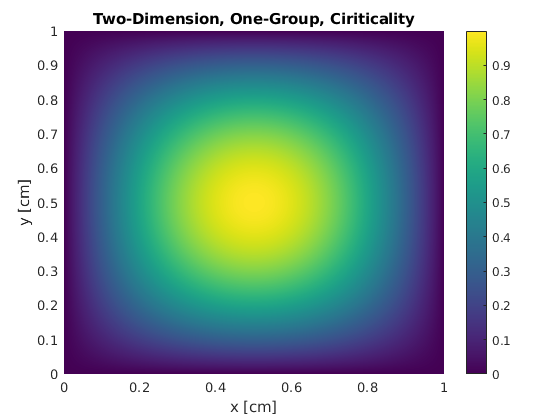
\includegraphics[width=0.7\textwidth]{2d1g}
    \label{fig:2d1g}
  \end{figure}
  \begin{equation}
    \label{eq:analytic_2d1g}
    \phi(x,y) = \phi_0 \sin\left(\frac{\pi}{L_x} x\right) \, 
      \sin\left(\frac{\pi}{L_y} y\right)
  \end{equation}
\end{frame}

\begin{frame}{Three-Dimension, One-Group, Finite Cylinder}
  \begin{table}
    %\caption{Finite Cylinder Convergence Study Results.}
    \label{tab:finite_cyl}
    \begin{center}
      \resizebox{\textwidth}{!}{
      \begin{threeparttable}
      \begin{tabular}{cccccccccc}
        \toprule
        Refine & $\keff$ & $\keff$ error \units{\glsentryshort{pcm}} & $\keff$ ratio & \gls{rms} & 
          \gls{rms} ratio  & $\|\ve\|_{\infty}$ & $\|\ve\|_{\infty}$ ratio \\
        \midrule
        0     &0.895108&10160.26&4.18   &5.34E-02&2.57     &2.12E-01&1.62\\
        1     &0.972412&2429.90 &4.16   &2.07E-02&3.19     &1.31E-01&4.65\\
        2\tnote{$\dagger$}     &0.990870&584.06  &3.90   &6.50E-03&1.85     &2.81E-02&1.79\\
        3     &0.995215&149.61  &3.99   &3.51E-03&9.22     &1.57E-02&8.28\\
        4     &0.996336&37.48   &       &3.81E-04&         &1.90E-03&    \\
        Ref. & 0.996711 \\
        \bottomrule
      \end{tabular}
        \begin{tablenotes}
        \item[$\dagger$] Refinement ratio $\approx 1$ but next case $\approx
          8$.\\
          This is due to the movement of mesh nodes in the process of circular
          mesh regeneration.
        \end{tablenotes}
      \end{threeparttable}
    }
    \end{center}
  \end{table}
  \vspace{-0.35in}
  \begin{figure}
    \centering
    \subfloat{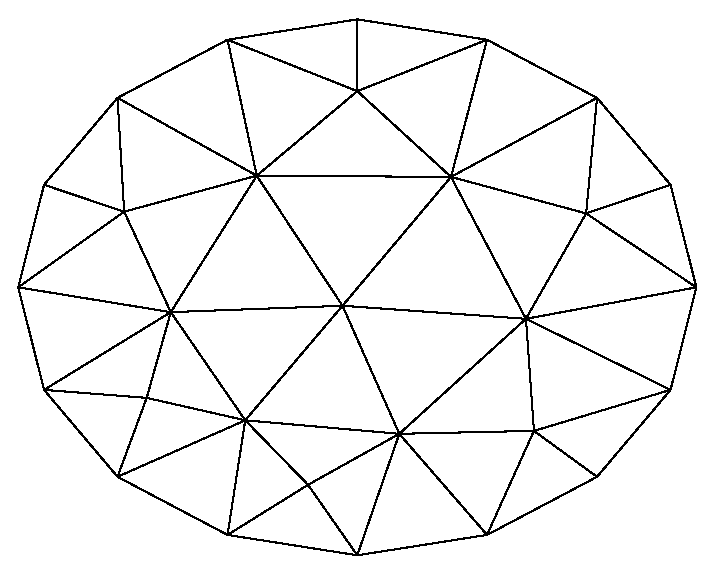
\includegraphics[width=0.35\textwidth]{cir0}}
    \hspace{0.25in}
    \subfloat{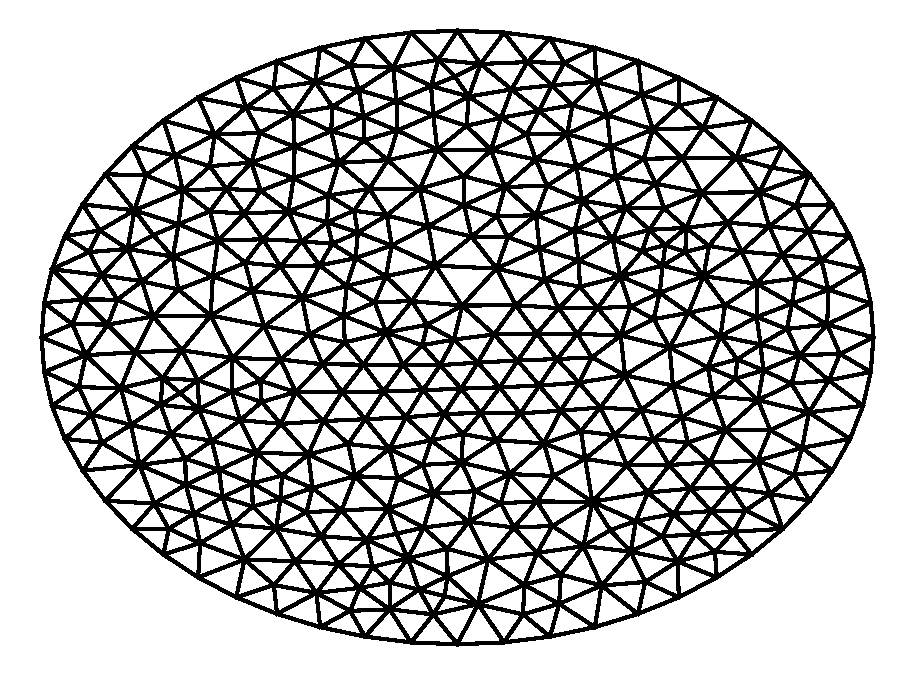
\includegraphics[width=0.35\textwidth]{cir2}}
    %\caption{Mesh Refinement of Curved Mesh.}
    \label{fig:circle_meshes}
  \end{figure}
\end{frame}

\begin{frame}{Three-Dimension, One-Group, Finite Cylinder}
  \begin{columns}
    \begin{column}{0.5\textwidth}
      \begin{figure}
        \centering
        \subfloat{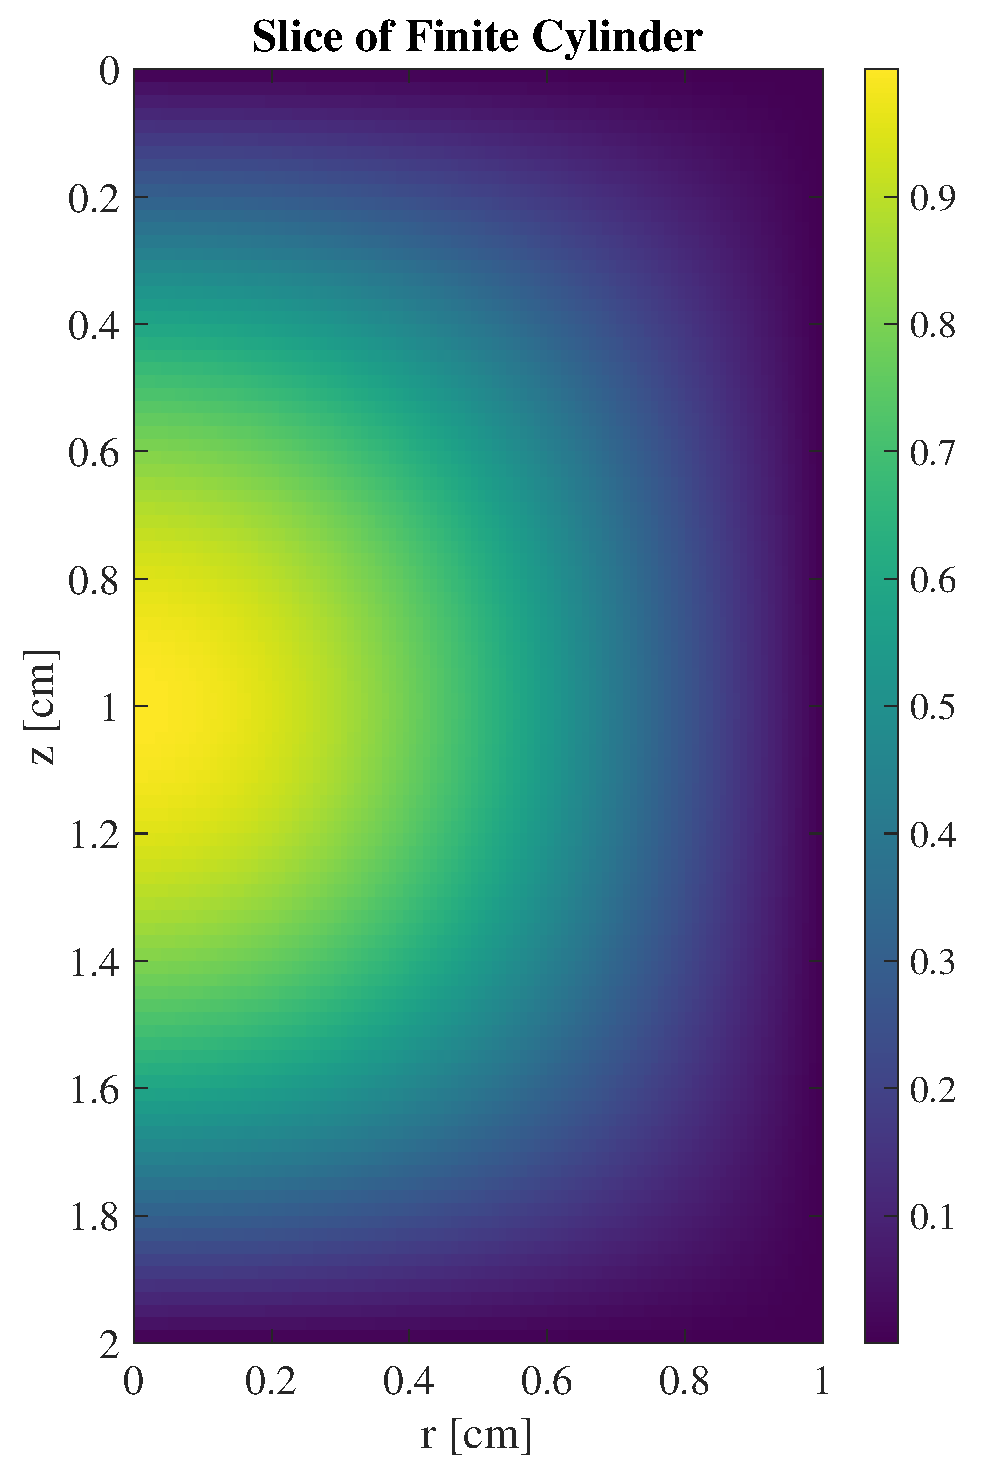
\includegraphics[width=0.7\textwidth]{finite_cyl}}
      \end{figure}
    \end{column}
    \begin{column}{0.5\textwidth}
      \begin{figure}
        \centering
        \vspace*{\fill}
        \subfloat{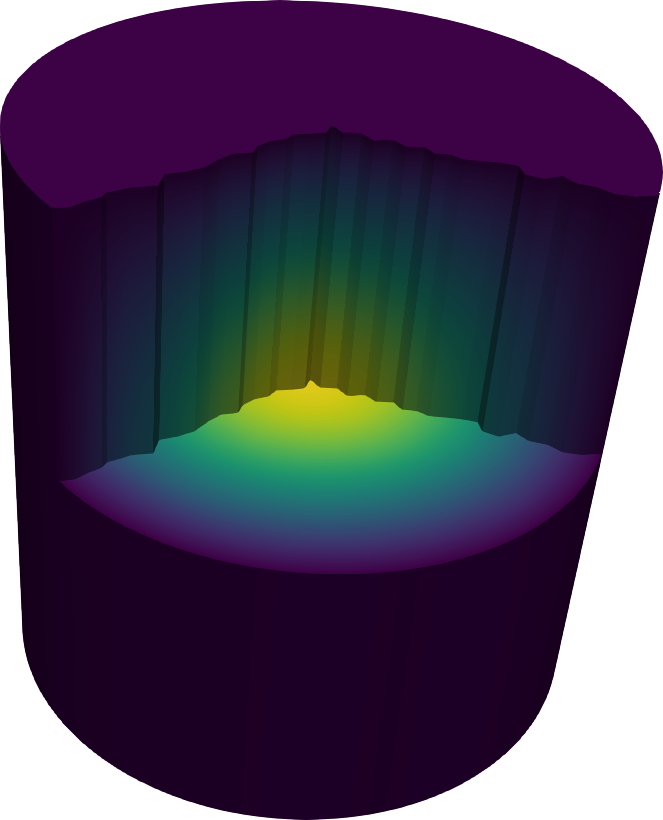
\includegraphics[width=0.8\textwidth]{./figs/finite_cyl_refine3}}
        \vspace*{\fill}
      \end{figure}
    \end{column}
  \end{columns}
  \begin{equation}
    \label{eq:analytic_finite_cyl}
    \phi(r,z) = \phi_0 \, 
      J_0\left(\frac{\alpha_0}{T} r\right) \sin\left(\frac{\pi}{H} z \right)
  \end{equation}
\end{frame}

\begin{frame}{Benchmark Solutions}
  \begin{itemize}
    \item 9 benchmark problems.
    \item Two and three dimensional geometry.
    \item Varied energy group structure and neutron spectrum.
  \end{itemize}
  \begin{table}
    %\caption{}
    %\label{}
    \begin{center}
      \resizebox{\textwidth}{!}{
      \begin{tabular}{lccccc}
        \toprule
        Benchmark & Dimensions & Groups & Reactor Type &
          \parbox[t]{0.6in}{\centering Neutron \\ Spectrum} \\
        \midrule
        VVER440 & 2 & 2 & \glsentryshort{lwr} & Thermal \\
        SNR     & 2 & 4 & \glsentryshort{sfr} & Fast \\
        \glsentryshort{hwr}     & 2 & 2 & \glsentryshort{hwr} & Thermal \\
        IAEA ($\times4$)    & 2 & 2 & \glsentryshort{pwr} & Thermal \\
        MONJU   & 3 & 3 & \glsentryshort{sfr} & Fast \\
        KNK     & 3 & 4 & \glsentryshort{sfr} & Fast \\
        \bottomrule
      \end{tabular}
    }
    \end{center}
  \end{table}
\end{frame}

\begin{frame}{VVER440}
  \begin{itemize}
    \item Two-dimensional.
    \item \gls{lwr}.
    \item Two-group.
  \end{itemize}
  \begin{table}
    \begin{center}
      %\caption{VVER440 Benchmark Convergence Study.}
      \label{tab:vver440}
      \begin{threeparttable}
        \begin{tabular}{cccc}
          \toprule
          Refine & $\keff$ & $\keff$ error \units{\glsentryshort{pcm}} \\
          \midrule
          \csvreader[
            late after line=\\,
            late after last line=\\,]
            {../ch03_diffusionResults/data/vver440.csv}{}
            {\csvcoli & \csvcolvi & \csvcolvii}
          Ref.\tnote{$\dagger$}  & 1.009700 \\
          \bottomrule
        \end{tabular}
        \begin{tablenotes}
          \item[$\dagger$] See \cite{chao}.
        \end{tablenotes}
      \end{threeparttable}
    \end{center}
  \end{table}
\end{frame}

\begin{frame}{VVER440 Benchmark Power Comparison}
  \vspace{-0.3in}
  \begin{figure}
    \centering
    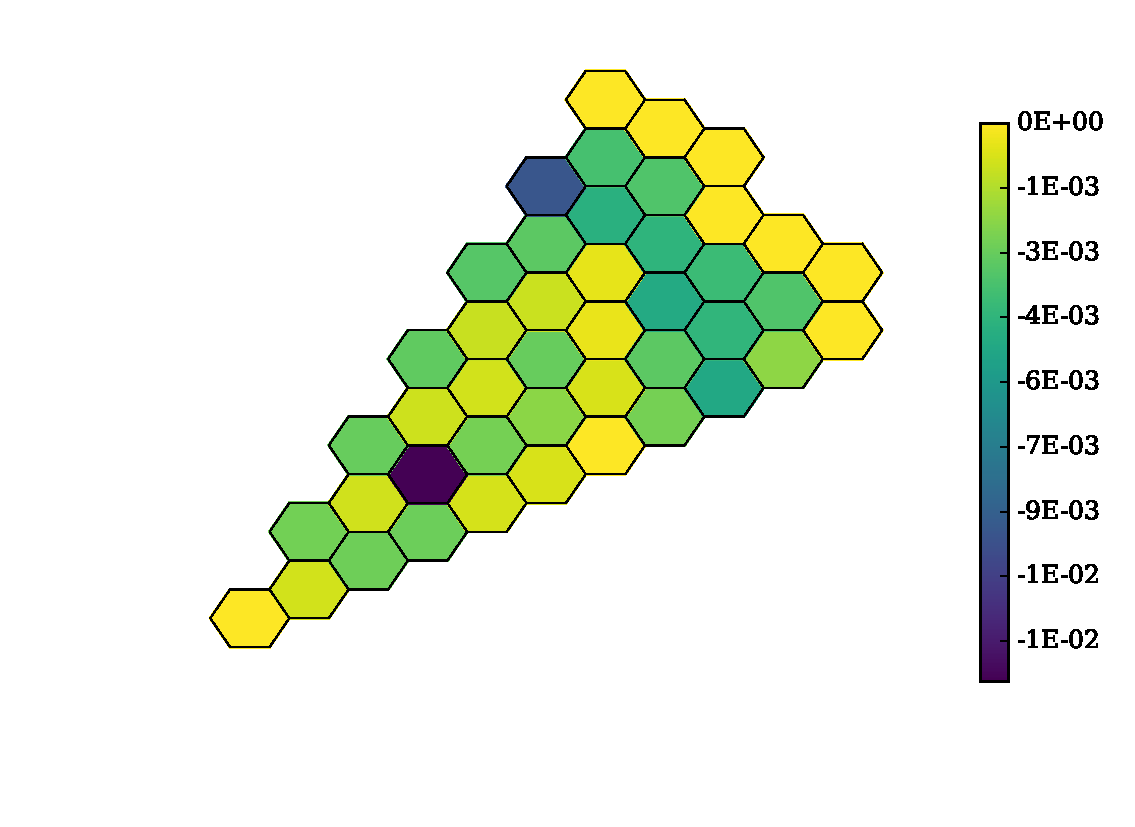
\includegraphics[width=\textwidth]{./figs/diffusion_vver440_colored}
    %\caption{VVER440 Benchmark Power Comparison for Most Refined Mesh.}
    \label{fig:diffusion_vver440}
  \end{figure}
  \vspace{-0.7in}
  \begin{center}
    VVER440 Benchmark Power Comparison for Most Refined Mesh.
  \end{center}
\end{frame}

\begin{frame}{MONJU}
  \begin{itemize}
    \item Three-dimensional.
    \item \gls{sfr}.
    \item Three-group.
    \item Case A. Control rods fully removed.
    \item Case B. Control rods partially inserted.
    \item Case C. Control rods fully inserted.
    %\item Fission spectrum, $\chi$ not provided and instead selected for
    %  benchmark agreement.
  \end{itemize}
  \begin{table}
    \begin{center}
      %\caption{MONJU Benchmark Rod Worth Results. \cite{monjuBenchmark}}
      \label{tab:monju}
      \begin{threeparttable}
        \begin{tabular}{ccll}
          \toprule
          Pattern & $\keff$ & Rod Worth \units{$\Delta k$} & 
            Rod Difference \units{\%$\Delta k$} \\
          \midrule
          A&1.056816&               &            \\
          B&1.031623&0.023 (2.51E-5) \tnote{$\dagger$} &2.52 (-0.07)\\
          C&1.006519&0.047 (1.77E-3)&5.03 (0.04) \\
          \bottomrule
        \end{tabular}
        \begin{tablenotes}
          \item[$\dagger$] Value in parentheses is difference to reference
            value \cite{monjuBenchmark}.
        \end{tablenotes}
      \end{threeparttable}
    \end{center}
  \end{table}
\end{frame}

\section{Thermal Hydraulics}
\label{sec:thermalHydraulics}

\begin{frame}{Enthalpy Rise}
  \begin{figure}
    \centering
    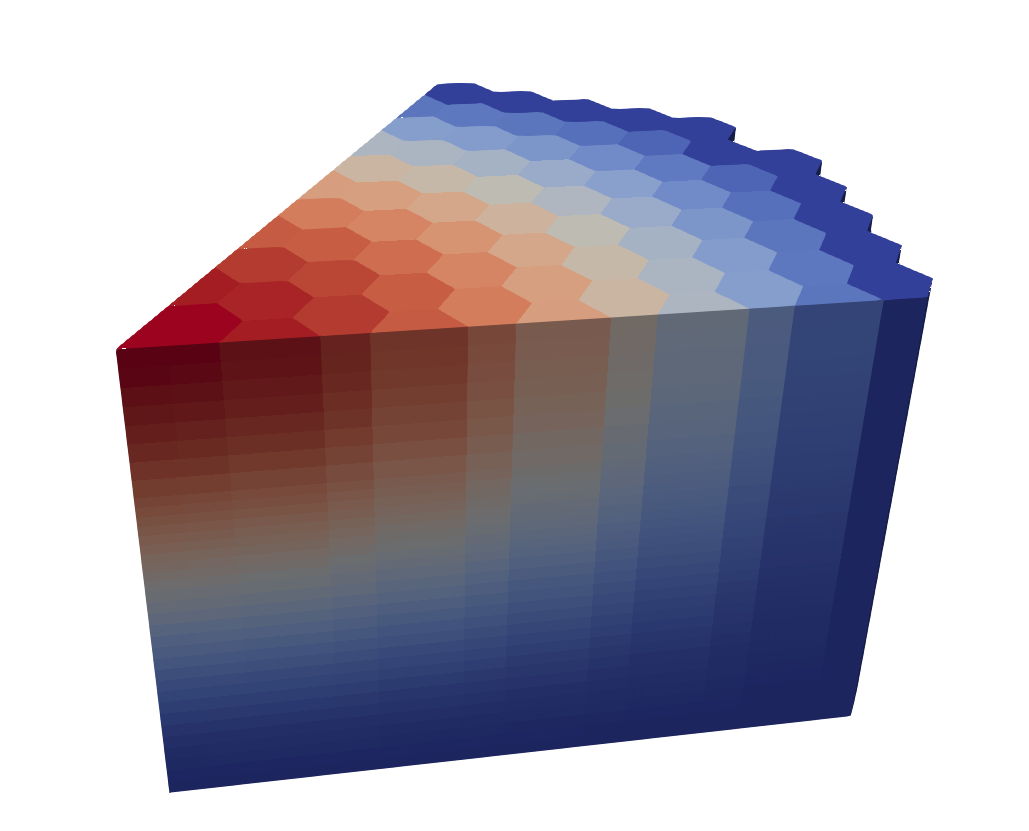
\includegraphics[width=0.8\textwidth]{enthalpy_rise}
    \caption{Typical SFR Enthalpy Rise.}
    \label{fig:enthalpy_rise}
  \end{figure}
\end{frame}

\begin{frame}{Material Temperatures}
  \vspace{-0.2in}
  \begin{figure}
    \begin{tabular}{cc}
      \subfloat[Cool]{
        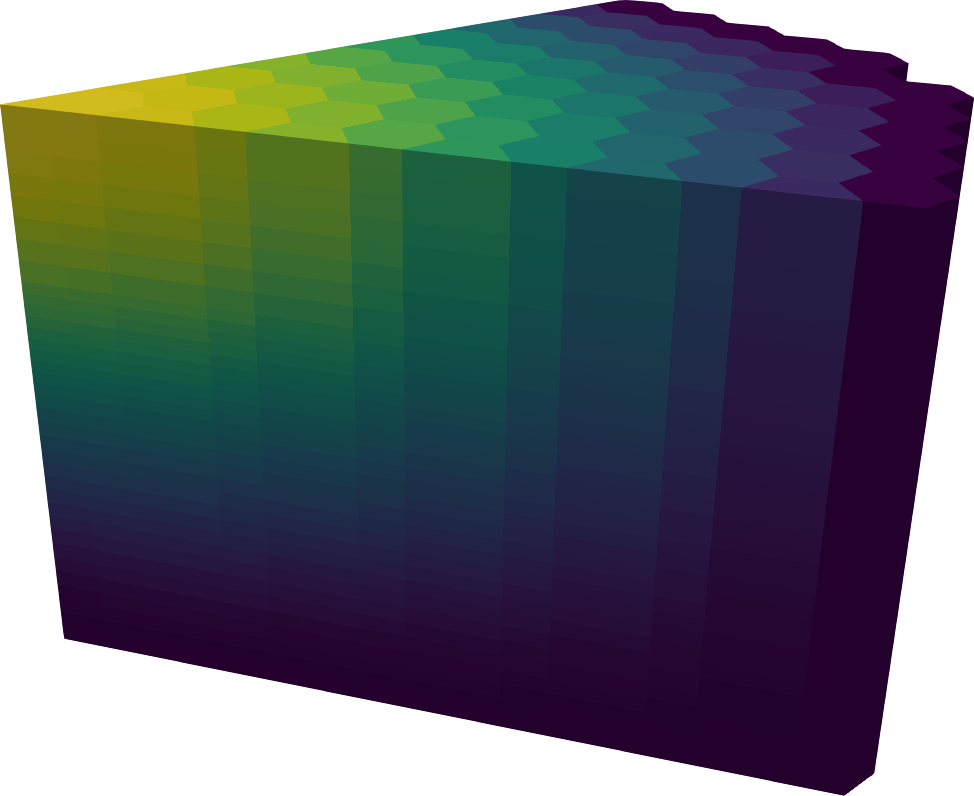
\includegraphics[width=0.35\textwidth]{./figs/temp_cool}} &
      \subfloat[Clad]{
        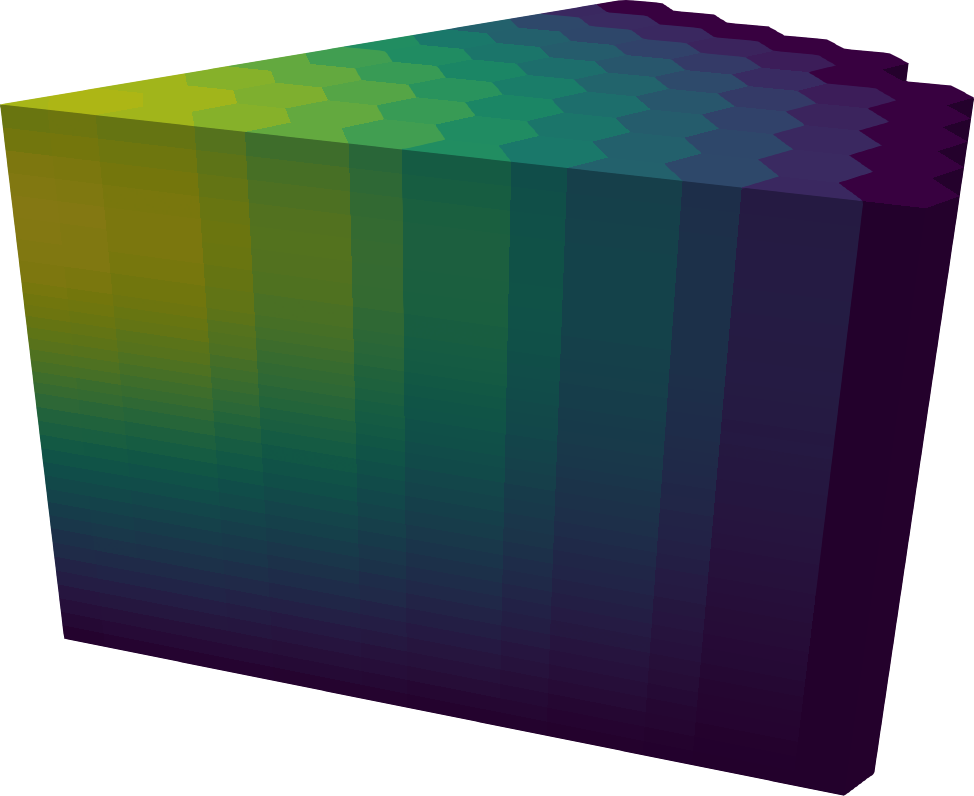
\includegraphics[width=0.35\textwidth]{./figs/temp_clad}} \\
      \subfloat[Bond]{
        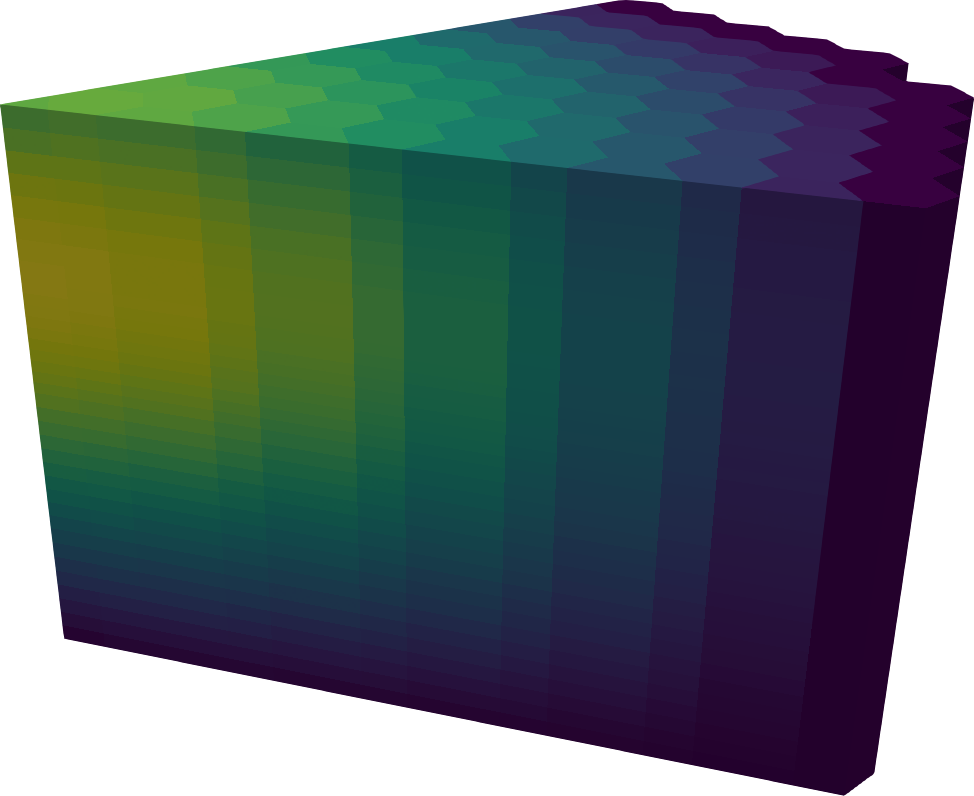
\includegraphics[width=0.35\textwidth]{./figs/temp_bond}} &
      \subfloat[Fuel]{
        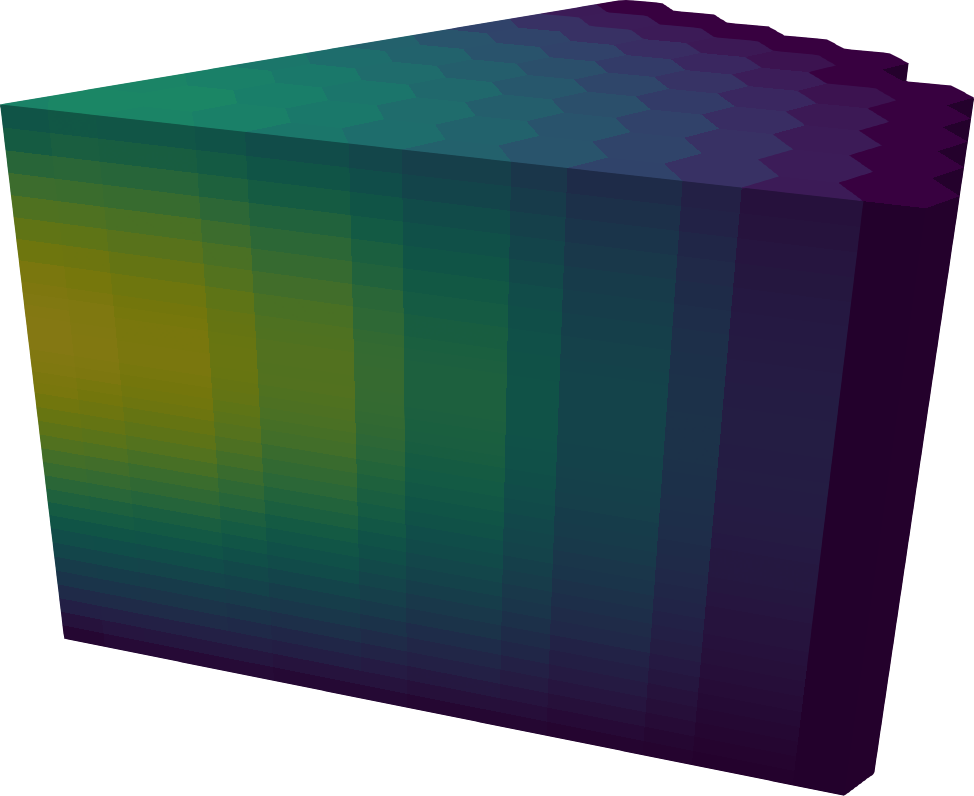
\includegraphics[width=0.35\textwidth]{./figs/temp_fuel}}
    \end{tabular}
    \caption{Typical SFR Average Material Temperatures.}
  \end{figure}
\end{frame}

\begin{frame}{Material Properties}
  \begin{itemize}
    \item Functional sodium properties from \cite{sodiumProp}.
    \item Temperature range of structural material small. 
    \item Clad and sodium thermal conductivity assumed constant \cite{ht9Prop}.
    \item Fuel thermal conductivity assumed a function of temperature
      \cite{fuelProp}.
  \end{itemize}
  \begin{table}
    \caption{Constant Thermal Conductivity for Sodium and HT9 at Reactor
      Temperatures.}
    \label{tab:constant_k}
    \begin{center}
      \begin{tabular}{cl}
        \toprule
        Material & $k \units{$\frac{\text{W}}{\text{m K}}$}$ \\
        \midrule
        Sodium &  64.33 \\
        HT9    &  25.81 \\
        \bottomrule
      \end{tabular}
    \end{center}
  \end{table}
\end{frame}

\begin{frame}{Thermal Conductivity}
  %\begin{align}
  %  \label{eq:kfuel_first}
  %  k_U      &= 21.73 + 1.591 \times 10^{-2} T + 5.907 \times 10^{-6} T^2 \\
  %  k_{Zr}   &= 8.853 + 7.082 \times 10^{-3} T + 2.533 \times 10^{-6} T^2 +
  %    2.992 \times 10^{3} T^{-1} \\
  %  k_{c,Zr} &= -102.0 + 200.1 x_{Zr} - 109.2 x_{Zr}^2 + 
  %    9.435 \times 10^{-3} T + 3.459 \times 10^{-5} T^2 - 0.02093 x_{Zr} \, T \\
  %  \label{eq:kfuel_last}
  %  k_{U-Zr} &= \left( 1 - \sqrt{1-x_{Zr}}\right) k_{Zr} + 
  %    \sqrt{1 - x_{Zr}} \left( \left( 1 - x_{Zr}\right) k_U + x_{Zr} \, k_{c,Zr}
  %    \right) 
  %\end{align}
  \begin{figure}
    \centering
    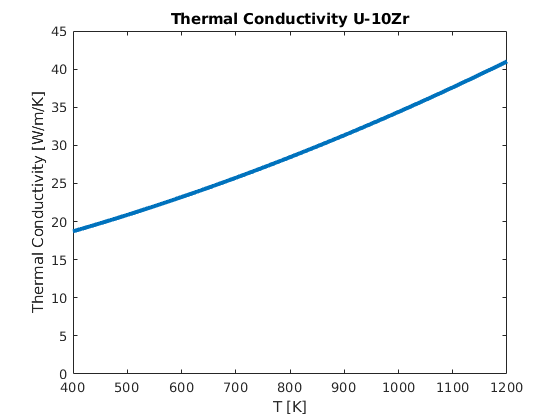
\includegraphics[width=0.7\textwidth]{kfuel_plot}
    %\caption{Variable Thermal Conductivity in Fuel.}
    \label{fig:kfuel_plot}
  \end{figure}
\end{frame}

\begin{frame}{Axial Convection Geometric Model}
  \begin{columns}
    \begin{column}{0.5\textwidth}
      \begin{figure}
        \centering
        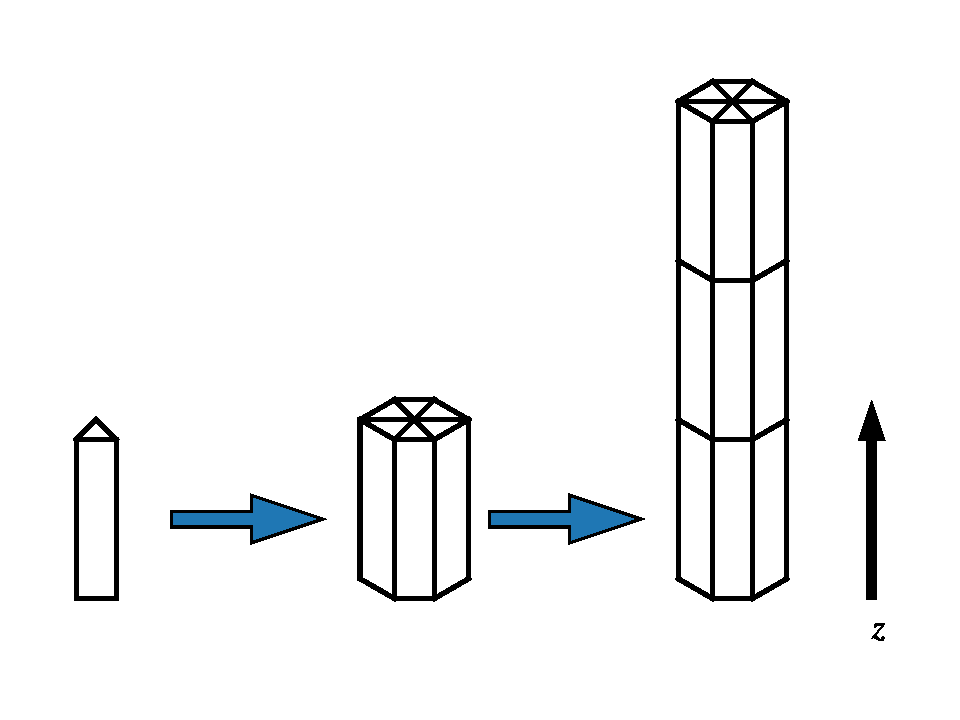
\includegraphics[width=\textwidth]{chunk_description}
        \caption{Progression of Element (left), to Chunk (center), to Channel
          (right).}
        \label{fig:chunk_description}
      \end{figure}
    \end{column}
    \begin{column}{0.5\textwidth}
      \begin{figure}
        \centering
        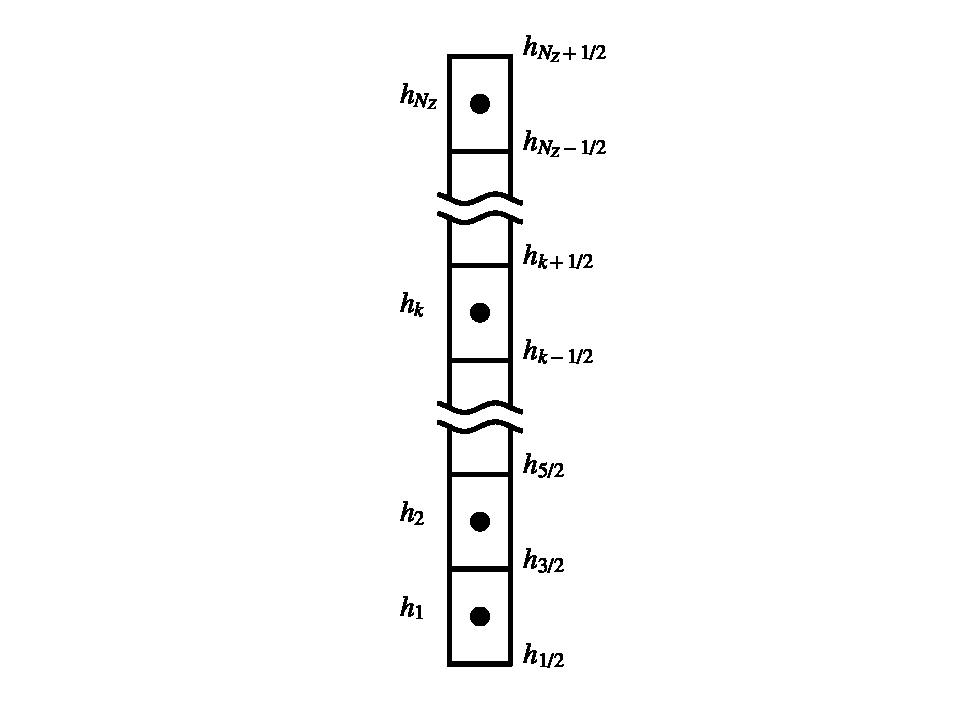
\includegraphics[width=0.35\textwidth]{axial_model}
        %\caption{One-Dimensional Axial Heat Convection Model Description.}
        \caption{Nodalization for channel $i$.}
        \label{fig:axial_model}
      \end{figure}
    \end{column}
  \end{columns}
\end{frame}

\begin{frame}{Channel Enthalpy}
  Steady-state coolant enthalpy within the channel is given by an energy
  balance.
  \begin{equation}
    h_{i,k+1/2} = h_{in} + \frac{1}{\mdot_i} \sum_{k=1}^{N_z} q_{i,k}
  \end{equation}
  Use a first-order approximation to estimate the chunk-average enthalpy.
  \begin{equation}
    h_{i,k} = \half (h_{i,k-1/2}+h_{i,k+1/2})
  \end{equation}
  $T_{\infty,i,k}$ is then given by a state relationship \cite{sodiumProp}.
  \begin{equation}
    T_{\infty,i,k} = T(h_{i,k})
  \end{equation}
\end{frame}

\begin{frame}{Radial Conduction Geometric Model}
  \begin{figure}
    \centering
    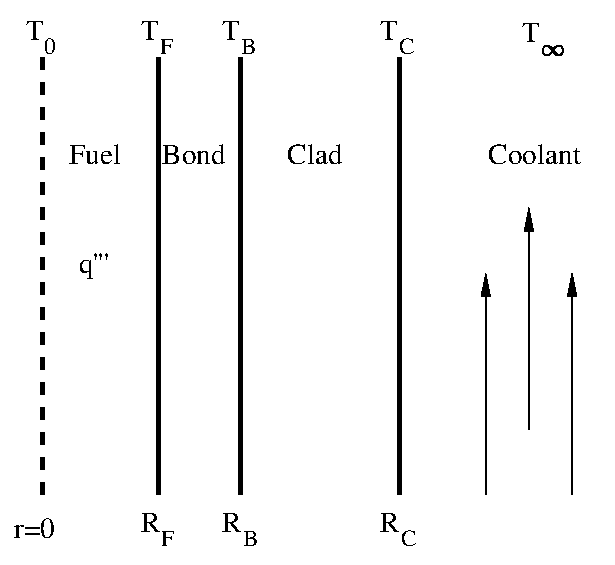
\includegraphics[width=0.7\textwidth]{radial_model}
    \caption{Geometry Description of Radial Heat Conduction Model (not to
      scale).}
    \label{fig:radial_model}
  \end{figure}
\end{frame}

\begin{frame}{Clad Surface Temperature -- Subbotin-Ushakov}
  Using Newton's Law of Cooling.
  \begin{align}
    q''_{clad} &= H_c (T_C - T_{\infty}) %\\
    %q''_{clad} &= q'''_{i,k} \frac{R_F^2}{2 R_C}
  \end{align}
  $H_c$ is given by the Subbotin-Ushakov correlation \cite{subbotinUshakov}
  which relates the Nusselt and P\'eclet numbers for ${1 < Pe < 4,000}$ and 
  ${ 1.2 \le S/D \le 2.0 }$.
  \begin{align}
    Pe &= Re \, Pr \\
    \label{eq:subbotinUshakov}
    Nu &= 7.55 \frac{S}{D} - 20 \left(\frac{S}{D}\right)^{-13} + 
      \frac{3.67}{90\left(\frac{S}{D}\right)^{2}}
      Pe^{\left(0.56 + 0.19 \frac{S}{D}\right)}
  \end{align}
  Then the clad surface temperature, $T_C$ follows.
  \begin{align}
    H_c &= \frac{N\!u \, k}{D_e} %\\
    %T_C &= \frac{q''_{clad}}{H_c} + T_{\infty}
  \end{align}
\end{frame}

\begin{frame}{Rod Surface Temperatures}
  Subsequent surface temperatures are given by radial heat conduction.
  \begin{align}
    \label{eq:tc_forward}
    T_C &= q'''_{i,k} \frac{R_F^2}{2\,R_c\,H_c} + T_{\infty} \\
    \label{eq:tb_forward}
    T_B &= T_C + \frac{q'''_{i,k}}{2 k_C} R_F^2
      \ln\left(\frac{R_C}{R_B}\right) \\
    \label{eq:tf_forward}
    T_F &= T_B + \frac{q'''_{i,k}}{2 k_B} R_F^2 
      \ln\left(\frac{R_B}{R_F}\right) \\
  \end{align}
\end{frame}

\begin{frame}{Fuel Centerline Temperature}
  Define a conductivity integral.
  \begin{equation}
    \label{eq:conductivity_integral}
    K_F(T) = \int_0^T k_F(T') \; dT'
  \end{equation}
  The value of the conductivity integral is given by the heat conduction
  equation.
  \begin{equation}
    \label{eq:tcl_conductivity_integral}
    K_F(T_0) = K_F(T_F) + \frac{q'''_{i,k}}{4} R_F^2
  \end{equation}
  Then, a bisection method search is used to calculate $T_0$ given a functional
  form of $K_F(T)$.
\end{frame}

\begin{frame}{Average Material Temperatures}
  Average temperatures in the clad and bond are calculated analytically.
  \begin{align}
    \label{eq:tc_bar}
    \overline{T_C} &= T_B - \frac{q'''}{4 k_C} R_F^2 \left(
      \frac{2 \, R_C^2 \ln\left(\frac{R_C}{R_B}\right)}
      {R_C^2 - R_B^2}  - 1\right) \\
    \label{eq:tb_bar}
    \overline{T_B} &= T_F - \frac{q'''_{i,k}}{4 k_B} \, R_F^2 \, \left(
      \frac{R_F^2 - R_B^2 + 2\,R_B^2 \ln\left(\frac{R_B}{R_F}\right)}
      {R_B^2-R_F^2}\right)
  \end{align}
\end{frame}

\begin{frame}{Average Fuel Temperature}
  To calculate an average fuel temperature, an effective fuel thermal
  conductivity is calculated.
  \begin{equation}
    \label{eq:kfuel_constant}
    \overline{k_F} = \frac{q'''_{i,k} \, R_F^2}{4(T_0-T_F)}
  \end{equation}
  Fuel thermal conductivity is assumed constant at $\overline{k_F}$ and an
  analytic value is calculated for the average fuel temperature.
  \begin{equation}
    \label{eq:tf_bar}
    \overline{T_F} = T_0 - \frac{q'''_{i,k}}{8 \overline{k_F}} R_F^2
  \end{equation}
  $\overline{T_F}$ is used to calculate fuel cross-sections. Due to
  self-shielding in the fuel, an effective fuel temperature would weight the
  surface temperature more.
\end{frame}

\begin{frame}{Radial Temperatures for Typical Fuel Rod}
  \begin{figure}
    \centering
    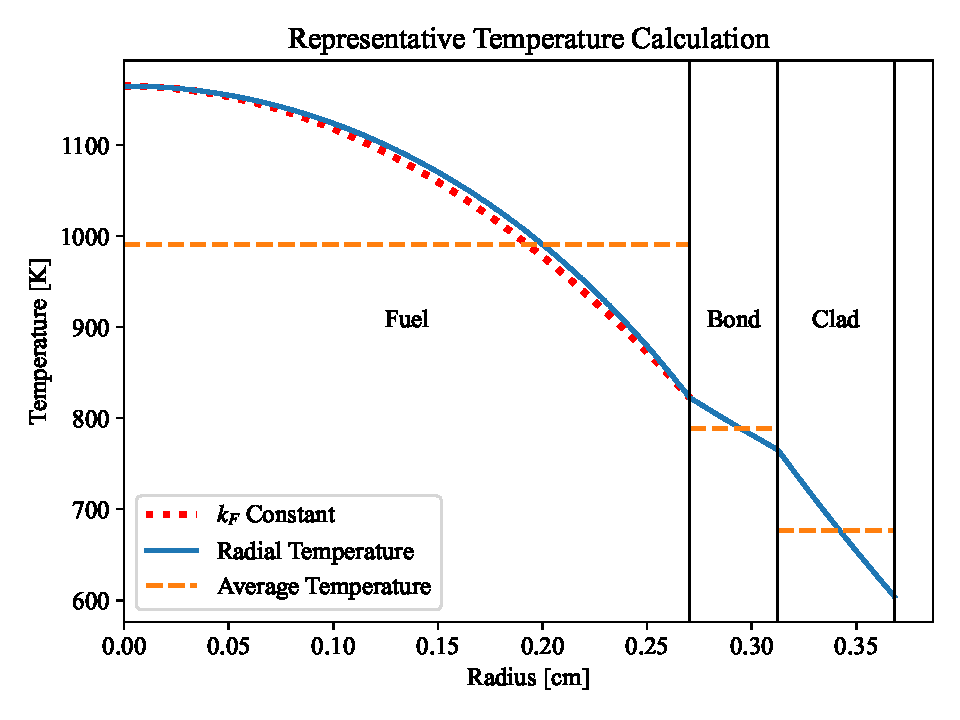
\includegraphics[width=0.7\textwidth]{radial_temp_plot}
    %\caption{Radial Temperatures for Typical Fuel Rod.}
    \label{fig:radial_temp_plot}
  \end{figure}
\end{frame}

\begin{frame}{Axial Temperatures for Typical Fuel Channel}
  \begin{columns}
    \begin{column}{0.5\textwidth}
      \begin{figure}
        \centering
        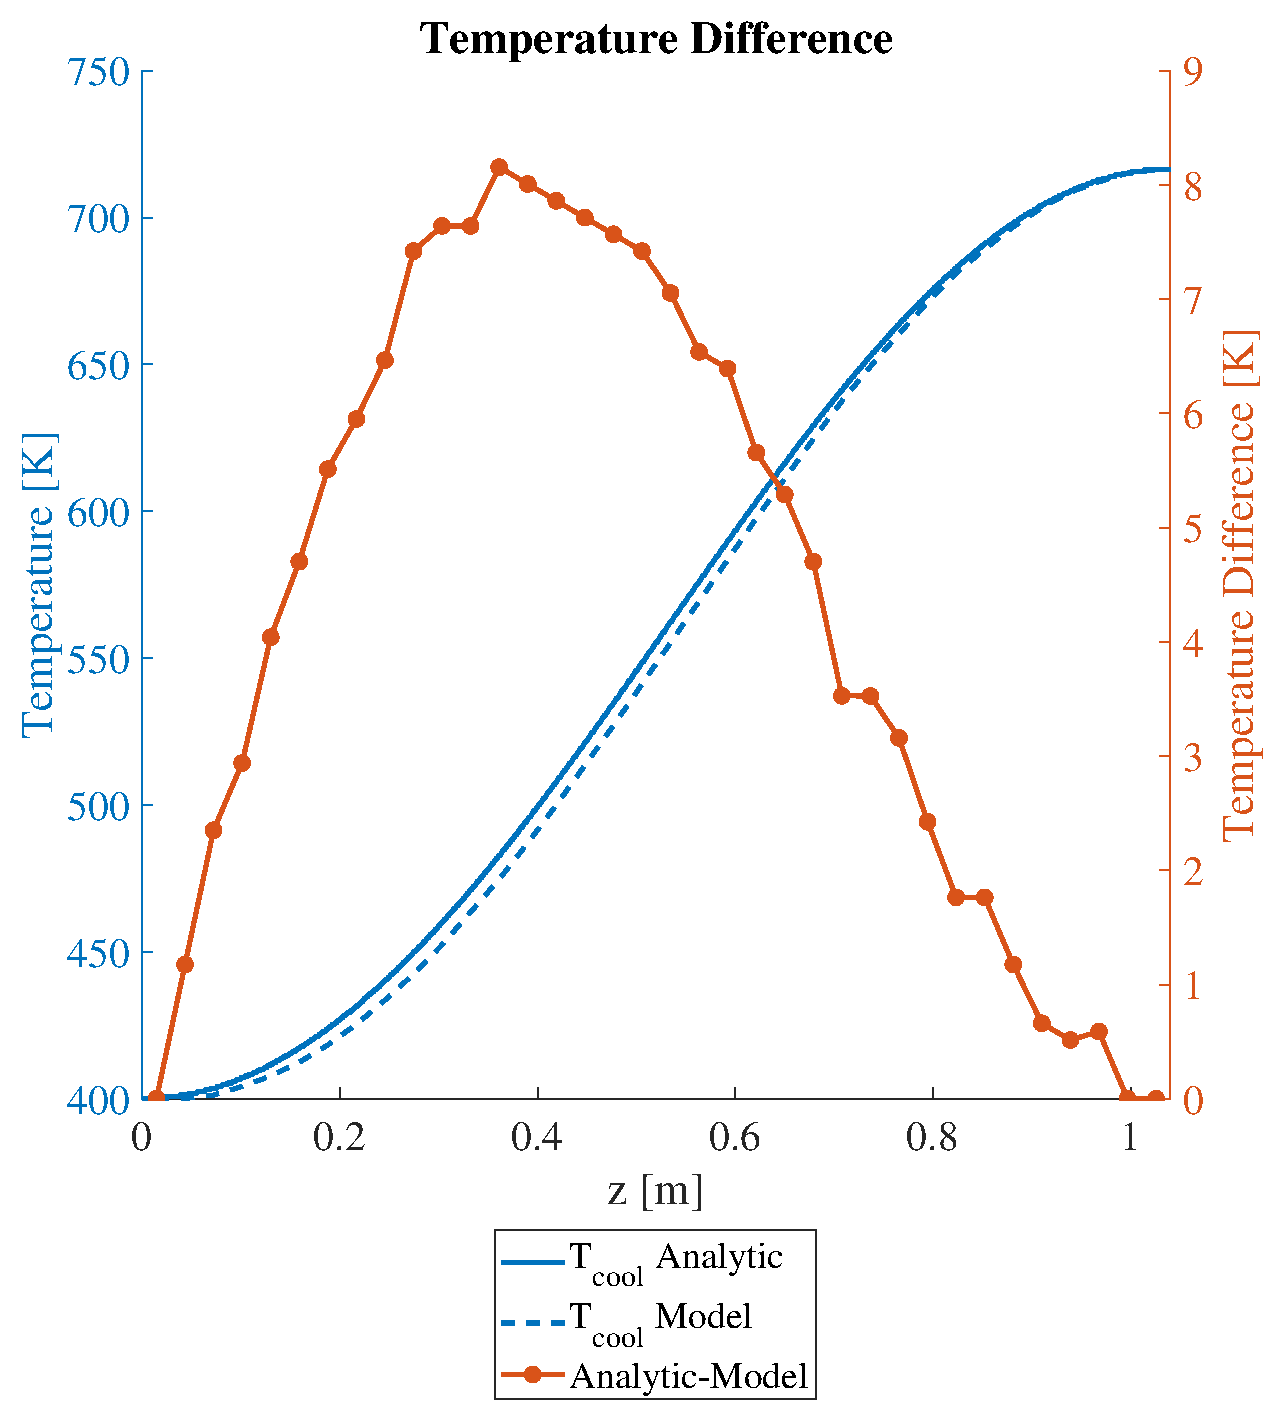
\includegraphics[width=\textwidth]{axial_difference_plot}
        %\caption{Difference Between Analytic and Modeled Axial Temperatures for 36
        %  Axial Levels.}
        \label{fig:axial_difference_plot}
      \end{figure}
    \end{column}
    \begin{column}{0.5\textwidth}
      \begin{figure}
        \centering
        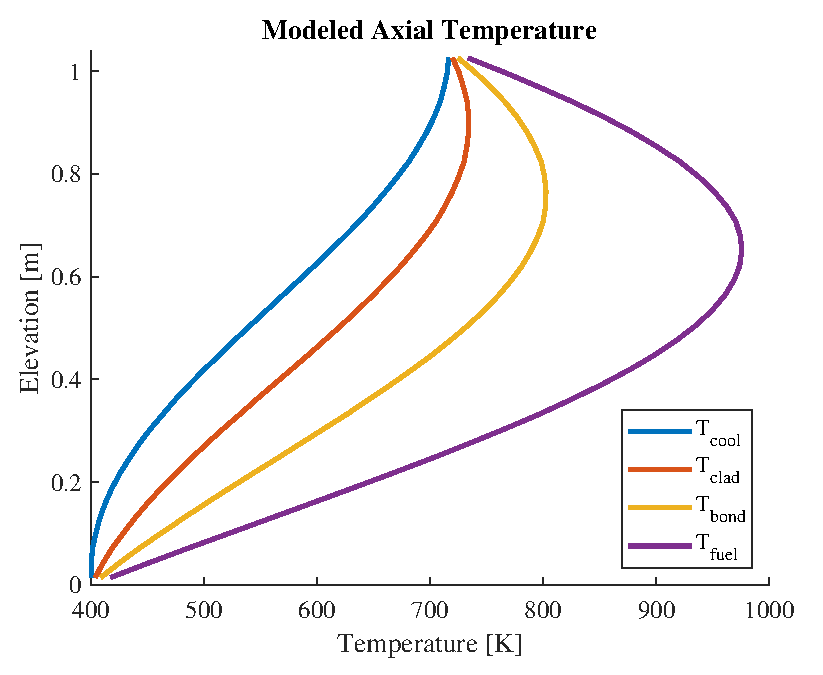
\includegraphics[width=\textwidth]{axial_temp_plot}
        %\caption{Average Axial Temperatures for Model Reactor Conditions.}
        \label{fig:axial_temp_plot}
      \end{figure}
    \end{column}
  \end{columns}
\end{frame}

%\begin{frame}{Cross-Section Treatment}
%  \begin{itemize}
%    \item Cross-sections are now unique to each chunk because temperatures are
%      unique to each chunk.
%    \item Coolant. 
%      \begin{itemize}
%        \item Number density and microscopic cross-sections are functionalized 
%          and updated based on $T_{\infty,i,k}$.
%        \item Linear interpolation for cross sections.
%      \end{itemize}
%    \item Clad. 
%      \begin{itemize}
%        \item Macroscopic cross-section updated based on $\overline{T_{C,i,k}}$.
%        \item Linear interpolation.
%      \end{itemize}
%    \item Bond.
%      \begin{itemize}
%        \item Assumed to have the same macroscopic cross-section as coolant.
%        \item Represents a small volume.
%        \item Consistent with homogenization approximation.
%      \end{itemize}
%    \item Fuel.
%      \begin{itemize}
%        \item Macroscopic cross-section update based on $\overline{T_{F,i,k}}$.
%        \item Square-root interpolation due to Doppler effect.
%      \end{itemize}
%  \end{itemize}
%\end{frame}

\begin{frame}{Cross-Section Treatment -- Coolant}
  \begin{itemize}
    \item Number density and microscopic cross-sections are functionalized 
      and updated based on $T_{\infty,i,k}$.
    \item Linear interpolation for cross sections.
  \end{itemize}

  Number density functionalization.
  \begin{align}
    \label{eq:number_density_sodium}
    M_{Na} &= 22.989769 \units{$\frac{\text{gram}}{\text{mol}}$} \\
    N_{Na}(T) &= \frac{\rho_{Na}(T) \, N_A}{M_{Na}}
  \end{align}

  Microscopic cross-section functionalization for ${T_{n} < T_{\infty,i,k} <
  T_{n+1}}$.
  \begin{equation}
    \label{eq:xs_cool}
    \Sigma_{x,i,k,g} = N_{Na}(T_{\infty,i,k}) 
      \left( \frac{T_{\infty,i,k} - T_{n}}{T_{n+1}-T_{n}} 
      (\sigma_{x,Na,g,n+1} - \sigma_{x,Na,g,n})  + \sigma_{x,Na,g,n}\right)
  \end{equation}
\end{frame}

\begin{frame}{Cross-Section Treatment -- Clad}
  \begin{itemize}
    \item Macroscopic cross-section updated based on $\overline{T_{C,i,k}}$.
    \item Linear interpolation.
  \end{itemize}

  Macroscopic cross-section functionalization for ${T_n < \overline{T_{C,i,k}} <
  T_{n+1}}$.
  \begin{equation}
    \label{eq:xs_linear_interpolation}
    \Sigma_{x,i,k,g} = 
      \frac{\overline{T_{C,i,k}} - T_{n}}{T_{n+1}-T_{n}} 
      (\Sigma_{x,g,n+1} - \Sigma_{x,g,n})  + \Sigma_{x,g,n}
  \end{equation}
\end{frame}

\begin{frame}{Cross-Section Treatment -- Bond}
  \begin{itemize}
    \item Assumed to have the same macroscopic cross-section as coolant.
    \item Represents a small volume.
    \item Consistent with homogenization approximation.
  \end{itemize}
\end{frame}

\begin{frame}{Cross-section Treatment -- Fuel}
  \begin{itemize}
    \item Macroscopic cross-section update based on $\overline{T_{F,i,k}}$.
    \item Square-root interpolation due to Doppler effect.
  \end{itemize}

  Macroscopic cross-section functionalization for ${T_n < \overline{T_{F,i,k}} <
  T_{n+1}}$.
  \begin{equation}
    \Sigma_{x,i,k,g} = 
      \frac{\sqrt{\overline{T_{F,i,k}}} - \sqrt{T_{n}}}
      {\sqrt{T_{n+1}}-\sqrt{T_{n}}}
      (\Sigma_{x,g,n+1} - \Sigma_{x,g,n})  + \Sigma_{x,g,n}
  \end{equation}
\end{frame}

\chapter{Thermal Expansion}
\label{ch:thermalExpansion}

\section{Necessity of Modeling}
  The Fast Reactor (FR) as modeled is entirely composed of
  metals and, as such, experiences significant thermal expansion. While other 
  designs may employ non-metallic fuel material (e.g. oxides or carbides), these 
  are not considered. Reactor designs with metal fuel include 
  Experimental Breeder Reactor II (EBR-II) as designed and built by Argonne 
  National Laboratory (ANL) and PRISM as designed by GE-Hitachi Nuclear Energy 
  (GEH).

  In metal fueled reactors such as EBR-II and PRISM, thermal expansion 
  represents a significant feedback effect and requires modeling. PRISM 
  estimates a thermal expansion feedback such that a 1\% change in radial 
  dimension results in $-0.5 \units{$\Delta k$}$ indicating a significant effect 
  \cite{GEFR793}. Additionally, thermal expansion has been proven to serve as an 
  inherent safety feature of SFRs. In the remarkable EBR-II demonstrations in 
  April 1986, two major accident events were performed on the reactor while 
  operating at full power. Operators forced the reactor to undergo Unprotected 
  Loss-Of-Flow (ULOF) and Unprotected Loss-Of-Heat-Sink (ULOHS) events. EBR-II 
  was safely shutdown due to nothing other than inherent thermal feedback 
  effects. These experiments demonstrated conclusively the passive safety of SFR
  designs due in part to the thermal expansion of materials 
  \cite{PlentifulEnergy}.

\section{Model Details}
  \label{sec:model_details}
  Highly detailed thermal expansion modeling can be performed using the Finite
  Element Method (FEM) to calculate local stresses and strains on all reactor
  structural components such as fuel pins, wire wraps, and assembly boxes. 
  However, the model developed here for the simulation of
  fast reactors does not estimate temperature and heat generation at all 
  positions due to the smearing of hexagonal assemblies. Therefore, a simplified 
  thermal expansion model is developed to simulate the effect of thermal 
  expansion on reactivity.

  In the model, linear dimensions are expanded based on material properties.
  All sodium in the reactor is assumed to be liquid so effects of thermal
  expansion within the sodium are assumed to be described by the change in
  density as a function of temperature as described by state equations in
  \cite{sodiumProp}. Additionally, the mass of sodium within the reactor is not
  conserved. In a Sodium-cooled Fast Reactor (SFR), sodium in the coolant is 
  allowed to flow into and out of an expansion vessel external to the reactor.
  The sodium in the bond region flows upward from the fuel region into a gas 
  plenum at the top of the fuel rod as the fuel expands. However, this is not 
  modeled as the sodium level in the bond is not tracked. Instead, the mass of 
  sodium in the bond region is allowed to vary during the simulation.

  \subsection{Material Properties}
    \label{sec:model_details__material_properties}
    All structural materials in the reactor are thermally expanded as HT9 
    stainless steel.
    Fuel material is thermally expanded as metallic uranium with 10\% Zr by 
    weight included (i.e. U10Zr). Thermal expansion properties for HT9 are given 
    in \cite{ht9Prop} and for U10Zr are given in \cite{thexpU10Zr}. The 
    equations for the Linear Expansion Factor (LEF) as functions of temperature 
    and used in this implementation are given
    \begin{equation}
      \label{eq:lef_ht9}
      \left( \frac{\Delta L}{L} \right)_{\text{HT9}} = 
        -2.191 \times 10^{-3} + 5.678 \times 10^{-6} \, T + 
        8.111 \times 10^{-9} \, T^2 - 2.576 \times 10^{-12} \, T^3 ,
    \end{equation}
    \begin{multline}
      \label{eq:lef_u10zr}
      \left( \frac{\Delta L}{L} \right)_{\text{U10Zr}} = \\
        \begin{cases}
          -7.3 \times 10^{-3} + 3.489 \times 10^{-5} \, T 
            - 5.154 \times 10^{-8} \, T^2 + 4.39 \times 10^{-11} \, T^3 & 
            T \le 923 \units{K} \\
          -0.25252 + 6.669 \times 10^{-4} \, T - 5.441 \times 10^{-7} \, T^2 
            + 1.518 \times 10^{-10} \, T^3 & \text{otherwise}
        \end{cases}
    \end{multline}
    for $T$ in \units{K}. Note that U10Zr undergoes a phase change at 
    $923 \units{K}$ that increases the LEF at this point. The LEF of HT9 and 
    U10Zr over the range of operating temperatures of fast reactors are plotted 
    in \fref{fig:lef_plot}. It is observed that the LEF of U10Zr is as much as 
    twice that of HT9. This implies fuel material will expand significantly more 
    than structural material which is expected behavior for metallic fuel.

    \begin{figure}
      \centering
      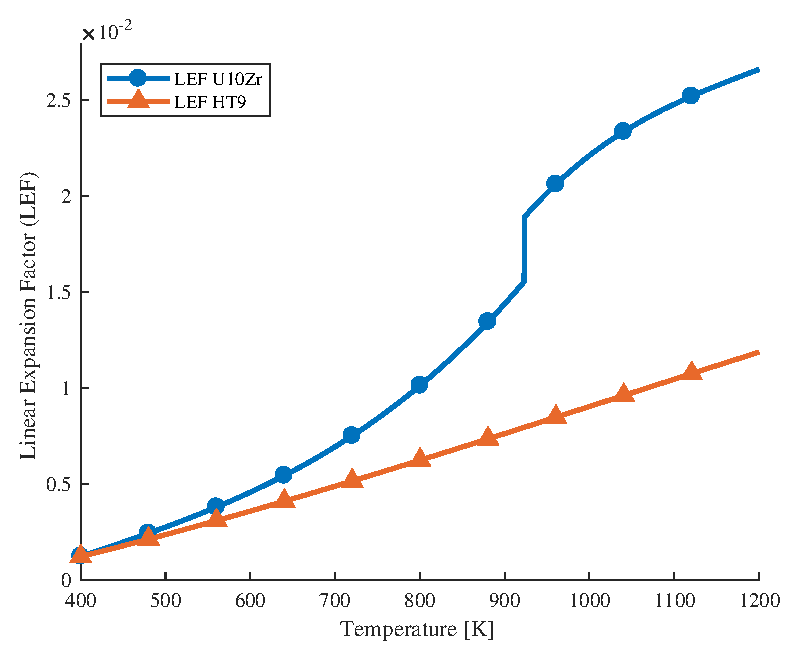
\includegraphics[width=0.7\textwidth]{lef_plot}
      \caption{Linear Expansion Factor for HT9 Steel and U10Zr Fuel.}
      \label{fig:lef_plot}
    \end{figure}
    
  \subsection{Assumptions and Formulae}
  \label{sec:model_details__assumptions_and_formulae}
    To simplify the modeling of thermal expansion, material dimensions are
    uniformly expanded in radial and axial directions. It is assumed that 
    material expansion in the radial direction (both $x$ and $y$ directions) 
    expands as HT9 because the dominating expansion in this direction is due to 
    the expansion of the hexagonal assemblies themselves and the grid plate at
    the base of the reactor. The exception to radial thermal expansion is that 
    the radius of the fuel, $R_F$, expands as U10Zr.  Within a hexagonal 
    assembly, the coolant flow area and the sodium bond area are allowed to 
    vary because of the assumption that the sodium is liquid.  It is assumed 
    that material expansion in the axial direction (the $z$ direction) expands 
    as U10Zr because the dominating expansion in this direction is the 
    elongation of the metallic fuel.
    
    All dimensions in the reactor are expanded assuming the user-input 
    dimensions are at room-temperature conditions. Dimensions are expanded
    according to two user-input temperatures, $\texpfuel$ and $\texpstruct$.
    $\texpfuel$ corresponds to the average temperature of reactor fuel and
    $\texpstruct$ corresponds to the average temperature of steel in the
    reactor. Typically, these values come from a previous coupled diffusion and
    thermal hydraulics simulation.
    It is expected thermal expansion 
    effects will be significant. However, thermal expansion factors are 
    typically on the order $10^{-6}$ so small, local changes in temperature are 
    not expected to affect the macroscopic simulation.

    Given the assumptions of this model, a radial LEF can be defined using 
    \eref{eq:lef_ht9} as
    \begin{equation}
      \label{eq:lef_r}
      F_r(\texpstruct) = \left(\frac{\Delta L}{L}\right)_{\text{HT9}}
    \end{equation}
    which is a function of $\texpstruct$. Note that given the assumption of 
    uniform radial thermal expansion, ${F_x(\texpstruct) = F_y(\texpstruct) =
    F_r(\texpstruct)}$.
    Similarly, an axial LEF can be defined using \eref{eq:lef_u10zr} as 
    \begin{equation}
      \label{eq:lef_a}
      F_a(\texpfuel) = \left(\frac{\Delta L}{L}\right)_{\text{U10Zr}}
    \end{equation}
    and $F_a(\texpfuel) = F_z(\texpfuel)$. For a ``cold'' cooridnate 
    $(x^C,y^C,z^C)$, the thermally expanded ``hot'' coordinate $(x^H,y^H,z^H)$ 
    can be expressed using radial and axial LEFs as
    \begin{align}
      \label{eq:expand_x}
      x^H &= x^C + x^C \, F_r(\texpstruct) \\
      \label{eq:expand_y}
      y^H &= y^C + y^C \, F_r(\texpstruct) \\
      \label{eq:expand_z}
      z^H &= z^C + z^C \, F_a(\texpfuel)
    \end{align}
    which is consistent with the assumption of uniform radial and axial 
    expansion. These formulae expand the distance from each coordinate to the
    origin, $(0,0,0)$.

    Using the coordinate transforms in \eref{eq:expand_x}, \eref{eq:expand_y}, 
    and \eref{eq:expand_z}, consider the thermal expansion of a cold volume 
    $V^C$. The volume is thermally expanded in the radial ($x$ and $y$) directions using
    \eref{eq:lef_r} and the axial ($z$) direction using \eref{eq:lef_a}. The
    volume $V^C$ has coordinate components $L_x^C$, $L_y^C$, and $L_z^C$
    such that ${V^C = L_x^C \, L_y^C \, L_z^C}$. This volume is shown with
    thermal expansion coefficients in \fref{fig:thexp_figure}.

    \begin{figure}
      \centering
      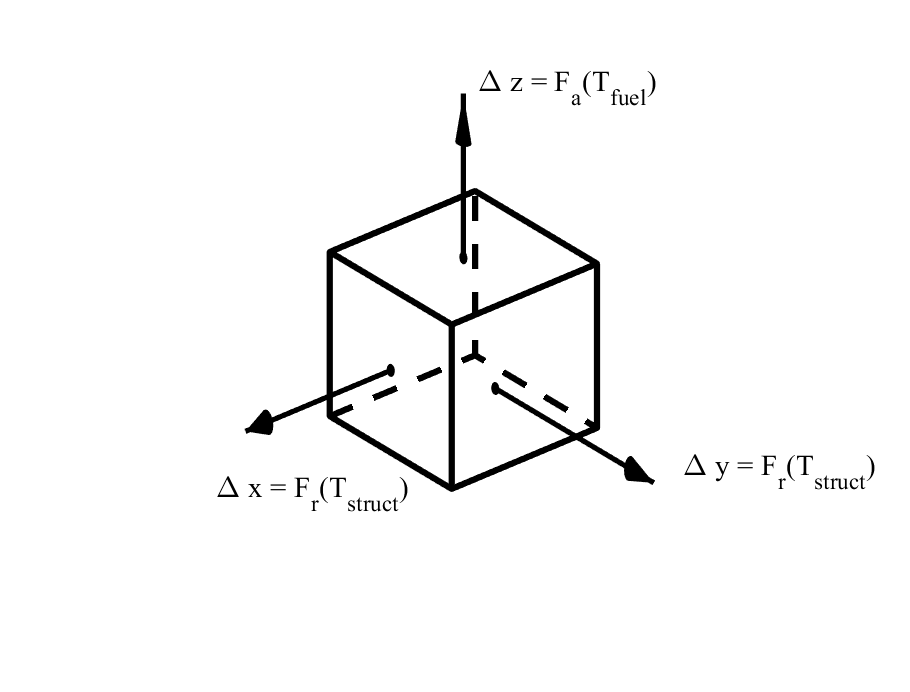
\includegraphics[width=0.7\textwidth]{thexp_figure}
      \caption{Thermal Expansion of General Volume.}
      \label{fig:thexp_figure}
    \end{figure}
    
    For the volume in \fref{fig:thexp_figure}, the thermally expanded 
    volume $V^H$ can be written
    \begin{align}
      V^H &= V^C + \Delta V, \\
      V^H &= (L_x^C + \Delta L_x) (L_y^C + \Delta L_y) (L_z^C + \Delta L_z). 
    \end{align}
    Then, recognizing the coordinate expansions,
    \begin{align}
      V^H &= (L_x^C + L_x^C \, F_r(\texpstruct)) + 
        (L_y^C + L_y^C \, F_r(\texpstruct)) + 
        (L_z^C + L_z^C \, F_a(\texpfuel)), \\
      V^H &= L_x^C \, L_y^C \, L_z^C \, (1 + F_r(\texpstruct))^2
        (1+F_a(\texpfuel)), \\
      V^H &= V^C (1 + F_r(\texpstruct))^2 (1+F_a(\texpfuel)).
    \end{align}
    The volume ratio is then
    \begin{equation}
      \label{eq:volume_ratio}
      \frac{V^C}{V^H} = \frac{1}{(1+F_r(\texpstruct))^2 (1+F_a(\texpfuel))}.
    \end{equation}
    Given the assumption of uniform thermal expansion in axial and radial
    directions, the ratio of volumetric expansion is constant throughout the
    reactor.

    The hexagonal assembly has total cross-sectional area $A$ and contains 
    component cross sections with areas $A_i$. For example, the total area 
    occupied by the fuel material could be considered $A_i$ and the total area 
    of the hexagon described by the flat-to-flat dimension could be considered 
    $A$. Define $A_i$ such that $\sum_{i} A_i = A$. Let the fractional area 
    $a_i = A_i/A$ and $\sum_{i} a_i = 1$.

    Using a method similar to the derivation of the volume ratio, a ratio can be
    derived for thermally expanded areas and area fractions. However, this would
    not be useful to the model because within an assembly, not all dimensions
    expand uniformly within the radial direction.
    The fuel radius and fuel area are expanded according to 
    $\left(\frac{\Delta L}{L_0}\right)_{\text{U10Zr}}$ whereas all other 
    materials are expanded according to 
    $\left(\frac{\Delta L}{L_0}\right)_{\text{HT9}}$. This does imply that,
    numerically, the radius of the fuel could exceed the inner radius of the 
    clad which is a non-physical result. This will only happen for small sodium 
    bond gaps and high thermal expansion temperatures. In these cases, the 
    radius of the fuel is confined to the expanded inner radius of the cladding.
    Though a more complex relationship describes the true value of these radii, 
    the error due to this assumption is small compared to the assumption of 
    uniform thermal expansion.
    
    Due to the different thermal expansions of fuel and structural material 
    within the cross-sectional area of the hexagonal assembly, the thermal 
    expansion of area fractions does not have a general formulaic relationship.
    Instead, area fractions are simply calculated at hot and cold conditions
    using expanded and unexpanded dimensions respectively. 

\section{Implementation}
  Thermal expansion affects the reactor in two major ways. First, thermal 
  expansion causes the physical dimensions of the reactor to increase. This is 
  modeled by the expansion of individual elements in the solution of the neutron 
  diffusion equation via the finite element method 
  (see \chref{ch:neutronDiffusion}) as well as the expansion of areas within the 
  hexagons. Second, as a result in the increase in physical dimensions, the 
  density of reactor materials decreases. This decrease in density is necessary
  to preserve the quantity of material within the reactor. In this derivation,
  the number of atoms in the reactor are conserved. The density change due to 
  thermal expansion is observed as a decrease in cross-sections.

  \subsection{Expansion of Elements and Area Fractions}
    Given the assumption of constant thermal expansion in radial and axial
    directions, thermal expansion follows immediately. Each node coordinate in
    the unstructured mesh is expanded according to \eref{eq:expand_x}, 
    \eref{eq:expand_y}, and \eref{eq:expand_z}. By expanding in axial and radial
    directions uniformly throughout the reactor, it is certain that there will 
    be no intersection or overlap of elements. In a realistic analysis, stress,
    strain, contact pressures, et cetera must be accounted for but this is 
    unnecessary here because the assumptions prohibit overlap and intersection 
    conditions.  As previously discussed in
    \sref{sec:model_details__assumptions_and_formulae}, the thermal expansion of
    area fractions is calculated directly.

  \subsection{Cross-section Effects}
    \label{sec:cross-section_effects}
    The conservation of reactor material is expressed as a conservation of 
    number of atoms. Allow the superscript $H$ to represent ``hot'' conditions 
    (i.e.  thermally expanded) and the superscript $C$ to represent ``cold'' 
    conditions.  Then, the conservation of the number of atoms for species $i$, 
    can be expressed as
    \begin{equation}
      \label{eq:conservation}
      n_i^H = n_i^C 
    \end{equation}
    where $n_i^H$ is the number of atoms of species $i$ after thermal expansion.
    The number of atoms $n_i$ can be written as 
    \begin{equation}
      \label{eq:nden_definition}
      n_i = N_i \, V_i
    \end{equation}
    where $N_i$ is the number density of species $i$ and $V_i$ is the volume
    occupied by species $i$. Then, inserting \eref{eq:nden_definition} into 
    \eref{eq:conservation} yields an expression for the thermally expanded 
    number density of species $i$ as
    \begin{align}
      N_i^H \, V_i^H &= N_i^C \, V_i^C, \\
      \label{eq:nden_volume_ratio}
      N_i^H &= N_i^C \frac{V_i^C}{V_i^H}
    \end{align}
    where the term $\frac{V_i^C}{V_i^H} < 1$ and represents the expansion of the
    volume occupied by species $i$. 

    The volume $V_i$ can be written in terms of element volume and area
    fraction. Let species $i$ be contained in region $j$ in finite element $e$. 
    This model assumes area fractions are constant within an element and can be
    treated as volume fractions. Then, the volume $V_i$ can be rewritten as 
    $V_i = a_j \, V_e$ where $a_j$ is the area fraction of region $j$ and $V_e$
    is the volume of the element $e$. Inserting this definition for $V_i$ into
    \eref{eq:nden_volume_ratio}.
    \begin{equation}
      \label{eq:nden_expansion_expanded}
      N_i^H = N_i^C \frac{a_j^C}{a_j^H} \frac{V_e^C}{V_e^H}
    \end{equation}
    Recall from \sref{sec:model_details__assumptions_and_formulae} that the
    ratio $\frac{a_j^C}{a_j^C}$ is dictated by the relative expansion of the
    fuel radius and the other structural materials. The area fractions
    themselves are calculated and the ratio is calculated subsequently. The 
    ratio $\frac{V_e^C}{V_e^H}$ is the standard volume ratio due to thermal 
    expansion and is given by \eref{eq:volume_ratio}. Inserting 
    \eref{eq:volume_ratio} into \eref{eq:nden_expansion_expanded}.
    \begin{equation}
      \label{eq:nden_thexp_update}
      N_i^H = N_i^C \frac{a_j^C}{a_j^H} 
        \frac{1}{(1+F_r(\texpstruct))^2 (1+F_a(\texpfuel))}
    \end{equation}
    Therefore, to preserve the number of atoms in the reactor, number densities
    in the reactor must be updated according to \eref{eq:nden_thexp_update} in
    addition to expanding reactor dimensions. Notice that
    \eref{eq:nden_thexp_update} can also be used to update neutron reaction 
    cross-sections directly as they are proportional to number density according
    to $\Sigma = \sigma N$.

\section{Results}
  The effect of thermal expansion on reactor criticality is observed. As
  previously mentioned in \sref{sec:model_details__assumptions_and_formulae}, 
  the user must input an effective temperature to which the reactor is thermally 
  expanded. This user-input values of $\texpstruct$ and $\texpfuel$ are varied 
  and all other thermal feedback effects are disabled in the simulation. It is 
  expected that thermal expansion will cause a significant decrease in $\keff$ 
  and represent negative reactivity insertion. Effective neutron multiplication 
  factor as a function of thermal expansion is plotted in \fref{fig:thexp_study} 
  and the associated reactivity, calculated as
  \begin{equation}
    \label{eq:reactivity_formula}
    \rho \units{pcm} = \frac{\keff - \kref}{\keff \, \kref} \times 10^5
  \end{equation}
  is plotted in \fref{fig:thexp_study_reactivity}. In
  \eref{eq:reactivity_formula}, $\keff$ is the calculated effective neutron 
  multiplication factor after thermal expansion and $\kref$ is the neutron 
  multiplication factor without thermal expansion. 

  Given the assumptions in this model, \fref{fig:thexp_study}  and
  \fref{fig:thexp_study_reactivity} show that thermal 
  expansion represents a significant reactivity effect and contributes as much 
  as $-1,000 \units{pcm}$ at extreme temperatures. Additionally, in this model 
  the thermal expansion factor of the fuel given in \eref{eq:lef_u10zr} 
  dominates and the phase change given by the formula can be seen at the 
  expected $923 \units{K}$.

  \begin{figure}
    \centering
    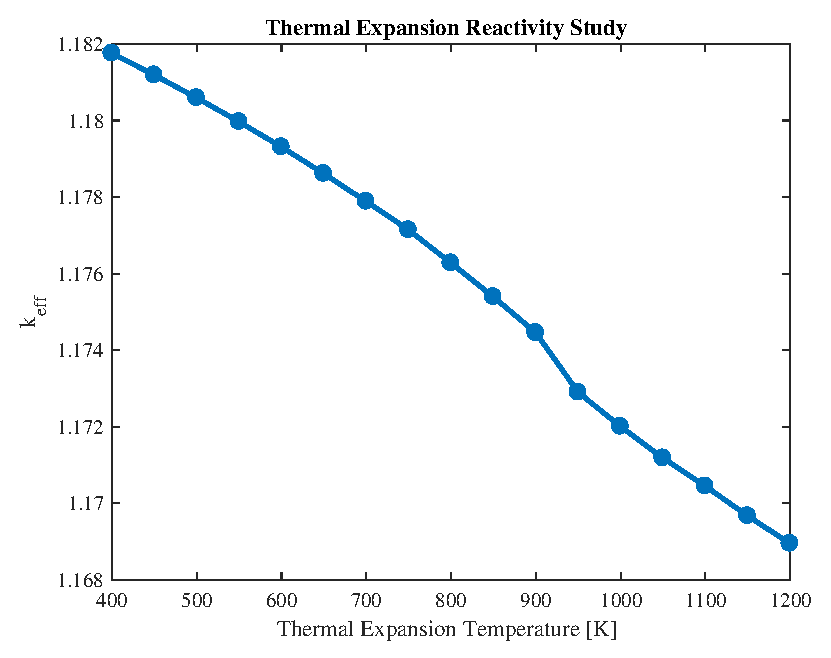
\includegraphics[width=0.7\textwidth]{thexp_study}
    \caption{Effective Neutron Multiplication Factor as a Function of 
      Thermal Expansion Temperature.}
    \label{fig:thexp_study}
  \end{figure}

  \begin{figure}
    \centering
    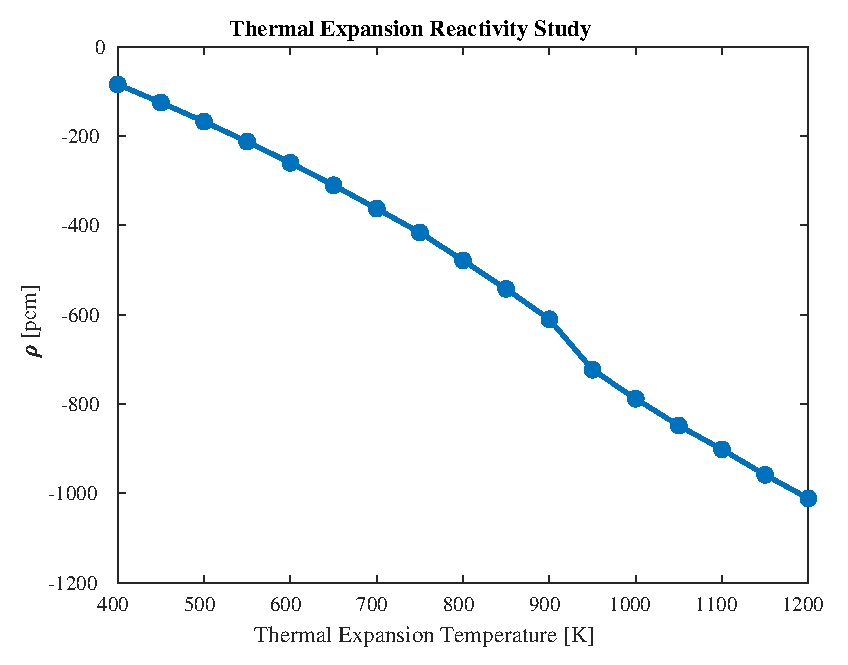
\includegraphics[width=0.7\textwidth]{thexp_study_reactivity}
    \caption{Reactivity as a Function of Thermal Expansion Temperature.}
    \label{fig:thexp_study_reactivity}
  \end{figure}

\chapter{Coupled Multiphysics Results}
\label{ch:coupledResults}

\section{Power Reactor Modeling}
\label{sec:power_reactor_modeling}
  The motivation for this work is to model nuclear power reactors with
  multiphysics feedback. This has been accomplished by modeling the reactor 
  power distribution with the multigroup neutron diffusion equation solved via 
  the Finite Element Method (FEM) (\chref{ch:neutronDiffusion}). Axial heat
  convection and radial heat conduction models are used to estimate reactor
  material temperatures (\chref{ch:thermalHydraulics}).
  Simplified thermal expansion modeling is used to model reactor dimensions 
  (\chref{ch:thermalExpansion}). Combined, these modeled multiphysics effects 
  will provide feedback which can be estimated in the model. 
  
  To test the coupling of these models, a realistic reactor benchmark is 
  provided and modeled \sref{sec:abr}. Reactivity coefficients describing system 
  feedback are defined in \sref{sec:reactivity_coefficients}. Results are 
  presented in \sref{sec:results}.

\section{Advanced Burner Reactor -- MET-1000}
\label{sec:abr}
  This reactor design is proposed by Organisation for Economic Co-operation and
  Development (OECD) Nuclear Energy Agency (NEA) \cite{abr}. The Advanced
  Burner Reactor (ABR) is fueled with a ternary metallic fuel and has a 1000
  \units{MWth} rating; hence, MET-1000. This is a medium-sized metallic reactor 
  with a total of 180 hexagonal assemblies and is 4.8 \units{m} tall. The 
  benchmark is fully specified and thirty-one independent results are submitted. 
  
  Each submission to the benchmark has generated its own cross-sections using 
  several different cross-section libraries (e.g. ENDFB7.0, JEFF3.1, etc.). 
  Therefore, using this benchmark as a verification problem is not feasible.
  Instead, cross-sections were generated for this model using \mcc and the
  procedure outlined in \sref{sec:cross_section_treatment}. This procedure 
  resulted  in temperature dependent cross-section libraries with 33 energy 
  groups. The  multigroup neutron diffusion equation is solved using these same
  cross-sections using both \dif and the method from \chref{ch:neutronDiffusion}.
  These two methods using the same cross-sections agree to within 700 
  \units{pcm}. The \dif and FEM models were minimally refined. A more formal 
  refinement study would presumably show further error reduction.

  The reactor materials in the benchmark are shown in \fref{fig:abr_materials}. 
  Though, the model used for benchmark comparison and subsequent reactivity
  coefficient calculations, the combined fast ($\phi_1$) and thermal ($\phi_2$)
  fluxes are plotted in \fref{fig:abr_fluxes}. Fast flux is shown to peak in
  the center of the core in the active fuel region. Thermal flux is shown to
  peak in core structural material, at the periphery of the active fuel region,
  as well as in control rod locations within the core.

  \begin{figure}
    \centering
    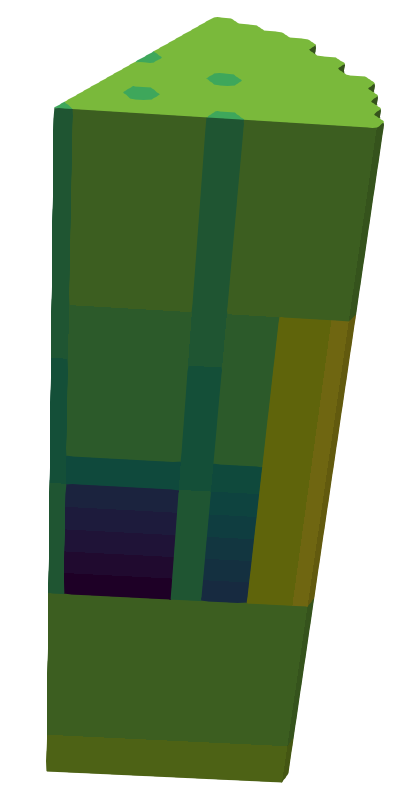
\includegraphics[width=0.4\textwidth]{abr_materials}
    \caption{Materials in ABR.}
    \label{fig:abr_materials}
  \end{figure}

  \begin{figure}
    \centering
    \subfloat[$\phi_{1}$]{
      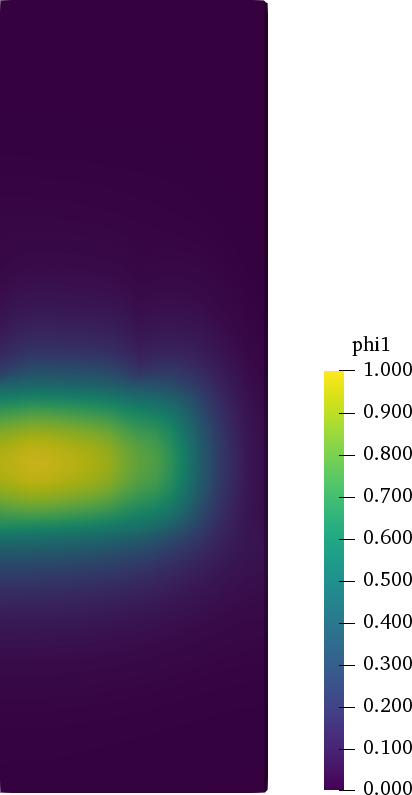
\includegraphics[width=0.25\textwidth]{abr_phi_nod_group1}}
    \hspace{0.2in}
    \subfloat[$\phi_{2}$]{
      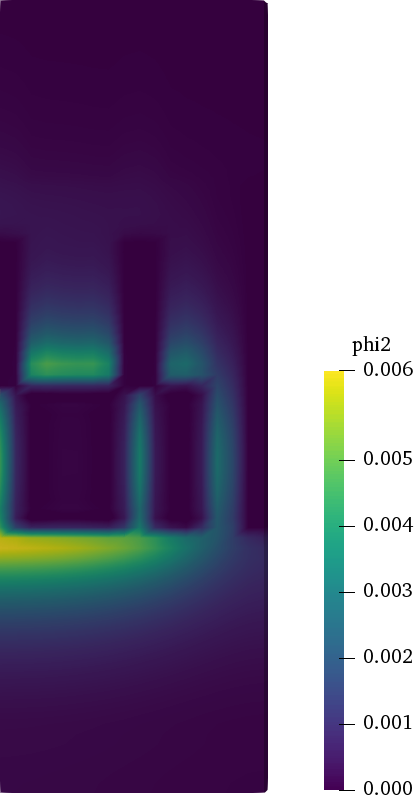
\includegraphics[width=0.25\textwidth]{abr_phi_nod_group2}}
    \caption{Fast (left) and Thermal (right) Neutron Flux in ABR.}
    \label{fig:abr_fluxes}
  \end{figure}

\section{Reactivity Coefficients}
\label{sec:reactivity_coefficients}
  Reactivity of a reactor can be used to compare the state of the reactor to the
  critical state. Reactivity $\rho$ is defined
  \begin{equation}
    \label{eq:reactivity}
    \rho \units{pcm} = \frac{\keff-1}{\keff} \times 10^5
  \end{equation}
  where \units{pcm} are units of percent-mille.
  Recall $\keff < 1$ for a subcritical reactor, $\keff=1$ for a critical
  reactor, and $\keff > 1$ for a supercritical reactor. Therefore $\rho < 0$
  for a subcritical reactor, $\rho = 0$ for a critical reactor, and $\rho > 0$
  for a supercritical reactor. 

  A reactivity coefficient can be defined as a partial derivative with respect
  to a quantity of interest \cite{textbookknief}. Let $\alpha_x$ be the 
  reactivity coefficient for quantity $x$, then
  \begin{equation}
    \label{eq:reactivity_coefficient}
    \alpha_x(x_i) = \left. \frac{\partial \rho}{\partial x} \right|_{x=x_i}
  \end{equation}
  where $\rho$ is the reactivity defined by \eref{eq:reactivity}.
  \eref{eq:reactivity_coefficient} is useful for estimating reactor dynamics.
  For some change in reactor state $\Delta x$, the reactivity response can be
  estimated as 
  \begin{equation}
    \label{eq:reactivity_estimate}
    \Delta \rho \approx \alpha_x(x_i) \, \Delta x.
  \end{equation}
  It is expected that reactivity coefficients will vary as reactor conditions
  vary. Therefore, it will be necessary to calculate $\alpha_x$ as a function of
  reactor condition $x_i$. Specifically, reactor power, $Q_{Rx}$, will be varied 
  in the calculation of $\alpha$. Therefore, consider a set of reactor powers
  varying from $0\%$ to $100\%$ as $Q_{Rx,i} = \{0\%,\ldots,100\%\}$.

  Reactivity coefficients useful for fast reactor applications include the power 
  coefficient, thermal expansion coefficient, fuel temperature (Doppler)
  coefficient, and coolant temperature coefficient (CTC) \cite{textbookknief}.
  Reactivity coefficients will be estimated with a first-order, forward-Euler,
  finite-difference approximation such that
  \begin{equation}
    \label{eq:reactivity_coefficient_finite_difference}
    \alpha_x(x_i) \approx \frac{\rho(x_i) - \rho(x_i + \Delta x)}{\Delta x}
  \end{equation}
  for a given $\Delta x$. The evaluation of
  \eref{eq:reactivity_coefficient_finite_difference} is discussed in the
  following sections for relevant reactivity coefficients.

  \subsection{Power Reactivity Coefficient}
  \label{sec:power_reactivity_coefficient}
    The power reactivity coefficient measures the reactivity response due to a 
    power increase. In a stable reactor, $\alpha_{power} < 0$ to ensure an 
    increase in reactor power requires a reactivity increase and to prevent a 
    runaway power increase. To evaluate $\alpha_{power}$, the reactor is
    simulated at a nominal reactor power, $Q_{Rx,i}$ resulting in
    $\keff(Q_{Rx,i})$. Then, reactor power is increased by $\Delta Q_{Rx}$
    resulting in $\keff(Q_{Rx,i} + \Delta Q_{Rx})$. These \keff values 
    correspond to reactivities $\rho(Q_{Rx,i})$ and 
    ${\rho(Q_{Rx,i} + \Delta Q_{Rx})}$ respectively as defined by 
    \eref{eq:reactivity}. With these values, the power reactivity coefficient 
    can be calculate as
    \begin{equation}
      \label{eq:power_reactivity_coefficient}
      \alpha_{power}(Q_{Rx,i}) = \frac{\rho(Q_{Rx,i}) - \rho(Q_{Rx,i} + 
        \Delta Q_{Rx})} {\Delta Q_{Rx}}.
    \end{equation}
    A typical value of $\Delta Q_{Rx}$ is $10\% \cdot Q_{Rx,i}$.
    % $10\% \, Q_{Rx,i}$.

  \subsection{Thermal Expansion Reactivity Coefficient}
  \label{sec:thermal_expansion_reactivity_coefficent}
    The thermal expansion reactivity coefficient describes the reactivity 
    response due solely to thermal expansion for a given increase in reactor 
    power. It is expected that thermal expansion will be the dominant 
    contribution to the power reactivity coefficient in fast reactors. This is 
    due to two main reasons: metal fuels expand significantly at high 
    temperature (see \chref{ch:thermalExpansion}) and the large neutron leakage 
    fraction (\leakage) in fast reactors \cite{PlentifulEnergy}. The leakage 
    fraction is the fraction of neutrons created in the fuel due to fission that 
    exit the core. Light Water Reactors (LWRs) typically have low and ultra-low 
    leakage designs with $\leakage \approx 2 \%$ \cite{textbookknief}. However,
    fast reactors simulated in this work have $\leakage \approx 20\%$ and 
    therefore are therefore highly sensitive to decreases in fuel density and 
    changing reactor dimensions due to thermal expansion.

    Thermal expansion temperatures, \texpfuel and \texpstruct, as implemented in 
    \chref{ch:thermalExpansion} must be known before the simulation. Note from
    \sref{sec:power_reactivity_coefficient}, a case must be simulated to
    calculate $\keff(Q_{Rx_i} + \Delta Q_{Rx})$ in the calculation of the power
    reactivity coefficient $\alpha_{power}$ in 
    \eref{eq:power_reactivity_coefficient}.  Therefore, the temperature
    distribution resulting from this study can be used to calculate the thermal
    expansion temperatures for the case with increased power, 
    ${\texp(Q_{Rx,i} + \Delta Q_{Rx})}$.
    Then, the thermal expansion reactivity coefficient is 
    \begin{equation}
      \label{eq:thermal_expansion_reactivity_coefficient}
      \alpha_{thexp}(Q_{Rx,i}) = \frac{\rho(\texp(Q_{Rx,i})) - 
        \rho(\texp(Q_{Rx,i} + \Delta Q_{Rx}))}
        {\Delta Q_{Rx}}
    \end{equation}
    where $\texp(Q_{Rx,i})$ represents the thermal expansion temperatures for
    power $Q_{Rx,i}$ and $\texp(Q_{Rx,i} + \Delta Q_{Rx})$ represents the
    thermal expansion temperatures for power $Q_{Rx,i} + \Delta Q_{Rx}$. Note
    that in \eref{eq:thermal_expansion_reactivity_coefficient}, only thermal
    expansion temperatures are changed, not the true reactor power $Q_{Rx}$.
    A typical value of $\Delta Q_{Rx}$ is $10\% \cdot Q_{Rx,i}$.
    %$10\% \, Q_{Rx,i}$.

  \subsection{Fuel Temperature (Doppler) Reactivity Coefficient}
  \label{sec:fuel_temperature_reactivity_coefficient}
    The fuel temperature reactivity coefficient measures the reactivity change 
    due to an increase in fuel temperature. This coefficient is often termed the
    Doppler coefficient because the reactivity effect is due to the Doppler
    broadening of resonance absorption peaks in heavy nuclei such as
    \isotope[238]{U} \cite{textbookknief}. Briefly, at high fuel temperatures, 
    neutrons are more likely to be parasitically absorbed by non-fissile nuclei
    than fissile-nuclei in the fuel material.

    To calculate $\alpha_{Doppler}$, fuel temperature is increased directly. A
    simulation is conducted with feedback for reactor power $Q_{Rx,i}$ and the
    temperature profile is stored. Then, the fuel temperature is uniformly 
    increased in the reactor by $\Delta T_{fuel}$ and the simulation is
    conducted again. This procedure will result in $\keff(Q_{Rx,i})$ and
    ${\keff(T_{fuel} + \Delta T_{fuel})}$. Associated reactivities can be
    calculated from \eref{eq:reactivity} and the Doppler reactivity coefficient
    follows.
    \begin{equation}
      \label{eq:doppler_reactivity_coefficient}
      \alpha_{Doppler}(Q_{Rx,i}) = \frac{\rho(Q_{Rx,i}) - \rho_i(T_{fuel} +
        \Delta T_{fuel})} {\Delta T_{fuel}}
    \end{equation}
    Note that the Doppler reactivity coefficient is always negative.
    A typical value of $\Delta T_{fuel}$ is $20\units{K}$.
    The definition in \eref{eq:doppler_reactivity_coefficient} is a
    \textit{uniform} Doppler coefficient as opposed to a \textit{distributed} 
    Doppler coefficient as temperatures are increased uniformly throughout the
    reactor.

  \subsection{Coolant Temperature Reactivity Coefficient (CTC)}
  \label{sec:coolant_temperature_reactivity_coefficient}
    The Coolant Temperature reactivity Coefficient (CTC) describes the
    reactivity change due to an increase in coolant temperature. In LWRs, this
    may be called the Moderator Temperature Coefficient (MTC) but in fast
    reactors, the coolant is not designed to moderate neutrons. Feedback in the 
    coolant is due to two main phenomena: the decrease in absorption 
    cross-sections in the coolant due to Doppler broadening and the decrease of 
    density due to temperature increase. The dominant effect is the decrease of 
    sodium density due to the temperature increase \cite{textbookknief}.

    Unlike all other reactivity coefficients presented here, the CTC of the ABR 
    is positive as is common in fast reactors. This implies increases in coolant 
    temperature will lead to an increase in reactivity and cause a subsequent 
    increase in reactor power. In fast reactors, the coolant acts as a parasitic 
    neutron absorber. Therefore, a decrease in the sodium absorption 
    cross-section encourages neutron absorption in fissile material in the fuel 
    resulting in a reactivity increase. This does not pose a stability problem 
    as long as the power reactivity coefficient remains negative.

    To calculate $\alpha_{CTC}$, coolant temperature is increased directly with
    a procedure similar to that for the Doppler reactivity coefficient in
    \sref{sec:fuel_temperature_reactivity_coefficient}. A simulation is 
    conducted with feedback for reactor power $Q_{Rx,i}$ and the temperature 
    profile is stored. Then, the coolant temperature is uniformly
    increased by $\Delta T_{cool}$ and the simulation is conducted again. This
    procedure will result in $\keff(Q_{Rx,i})$ and 
    ${\keff(T_{cool} + \Delta T_{cool})}$. The reactivity associated with each
    \keff can be calculated given \eref{eq:reactivity} and the coolant
    temperature coefficient is
    \begin{equation}
      \label{eq:coolant_temperature_reactivity_coefficient}
      \alpha_{CTC}(Q_{Rx,i}) = \frac{\rho(Q_{Rx,i}) - \rho(T_{cool} + 
        \Delta T_{cool})} {\Delta T_{cool}}.
    \end{equation}
    A typical value for $\Delta T_{cool}$ is $50 \units{K}$.

\section{Results}
\label{sec:results}
  Returning to the ABR MET-1000 benchmark, reactivity coefficients are modeled
  for this reactor. The methodology and formulae from
  \sref{sec:reactivity_coefficients} are used. The reactor \keff as a function
  of reactor power is plotted in \fref{fig:keff_effects}. Note \keff decreases
  as power increases and the \keff for the case with increased sodium
  temperature is higher than all other \keff.
  
  The coefficients themselves are plotted in 
  \fref{fig:abr_reactivity_coefficients}. The combined power reactivity
  coefficient is plotted in \fref{fig:power_reactivity_coefficient}. Note,
  $\alpha_{power} < 0$ for all powers. At low reactor power, the reactivity
  coefficient is dominated by the Doppler reactivity coefficient plotted in
  \fref{fig:doppler_reactivity_coefficient}. At moderate reactor powers,
  $\alpha_{power}$ becomes less negative due to the coolant temperature
  coefficient plotted in \fref{fig:coolant_temperature_reactivity_coefficient}.
  At high reactor powers, $\alpha_{power}$ becomes more negative due to the
  dominance of the thermal expansion reactivity coefficient plotted in
  \fref{fig:thermal_expansion_reactivity_coefficient}. Should reactor power
  continue to increase beyond $100\%$ nominal value, the power reactivity
  coefficient would continue to become more negative as thermal expansion will
  continue to dominate.

  \begin{figure}
    \centering
    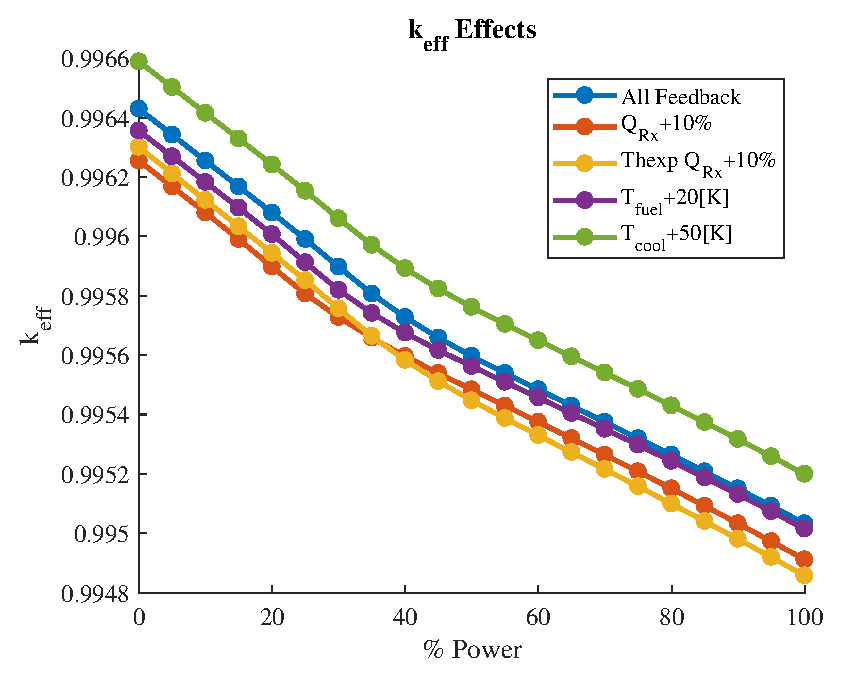
\includegraphics[width=0.7\textwidth]{keff_effects}
    \caption{Feedback Effects on \keff.}
    \label{fig:keff_effects}
  \end{figure}

  \begin{figure}
    \centering
    \subfloat[Power Reactivity Coefficient.]{
      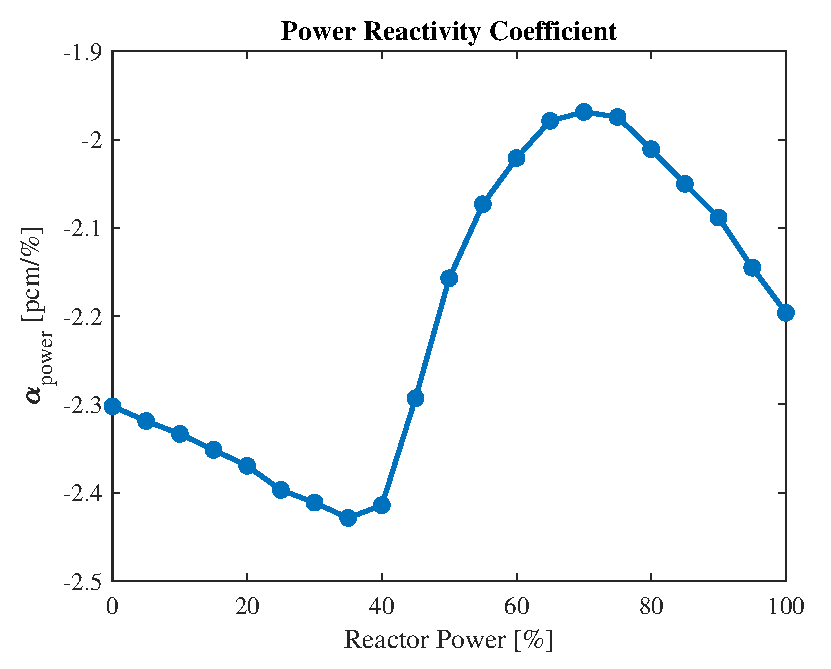
\includegraphics[width=0.5\textwidth]{alpha_power}
      \label{fig:power_reactivity_coefficient}}
    \hspace*{\fill}
    \subfloat[Thermal Expansion Reactivity Coefficient.]{
      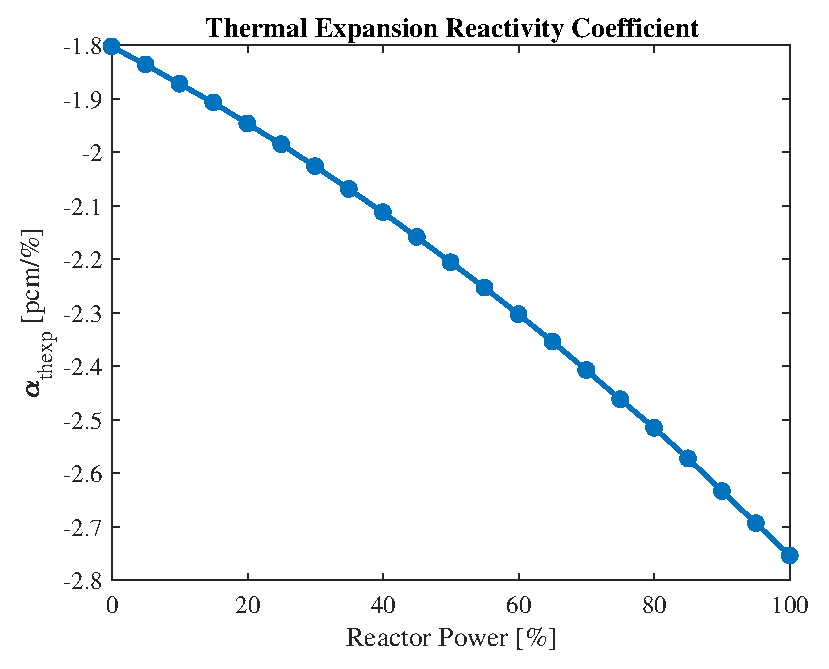
\includegraphics[width=0.5\textwidth]{alpha_thexp}
      \label{fig:thermal_expansion_reactivity_coefficient}}
    \vspace{\baselineskip}
    \subfloat[Doppler Reactivity Coefficient.]{
      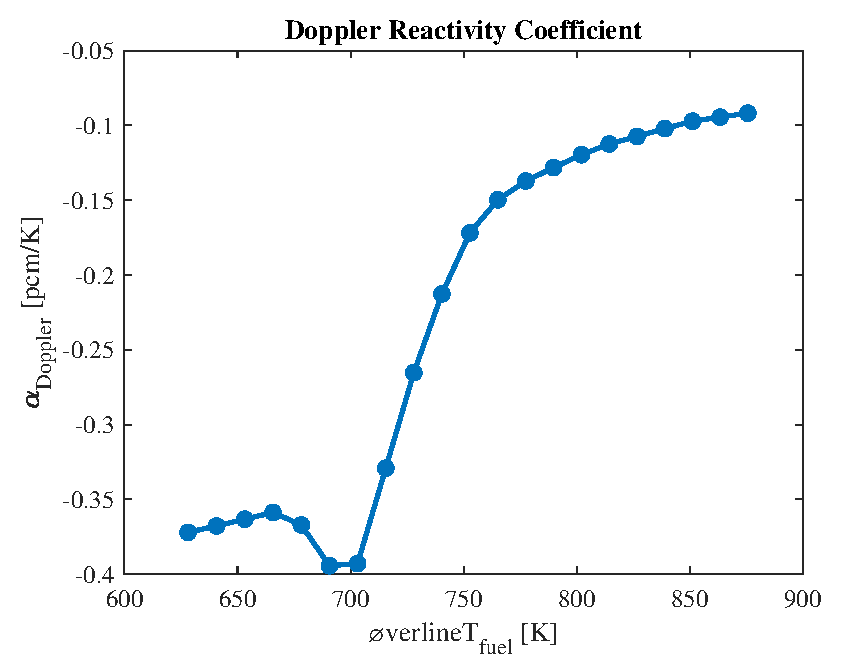
\includegraphics[width=0.5\textwidth]{alpha_fuel}
      \label{fig:doppler_reactivity_coefficient}}
    \hspace*{\fill}
    \subfloat[Coolant Temperature Reactivity Coefficient.]{
      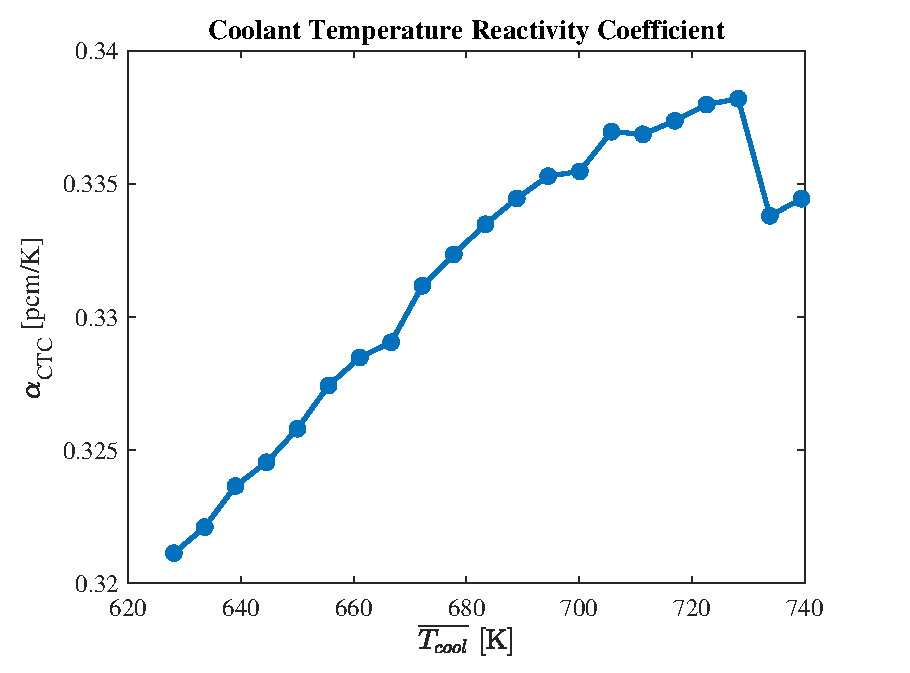
\includegraphics[width=0.5\textwidth]{alpha_cool}
      \label{fig:coolant_temperature_reactivity_coefficient}}
    \caption{ABR Reactivity Coefficients.}
    \label{fig:abr_reactivity_coefficients}
  \end{figure}

\chapter{Summary, Conclusions, and Recommendations}
\label{ch:conclusions}

\section{Overview of Simulation Results}

\section{Conclusions}

\section{Recommendations for Future Research}

  \subsection{Code Enhancements}
    \begin{itemize}
      \item Depletion
      \item Higher Order Elements
      \item SPN
      \item Enhanced Thermal Models
      \item Parallelization
    \end{itemize}

  \subsection{Further Investigations}
    \begin{itemize}
      \item SuperPhenix Benchmark
      \item EBR-II modeling
    \end{itemize}


\begin{frame}{Thank You!}
\end{frame}

\begin{frame}[allowframebreaks]{References}
  \printbibliography[heading=none]
\end{frame}

\begin{frame}[allowframebreaks]{Acronyms}
  \printglossary[type=\acronymtype,nonumberlist]
\end{frame}

\begin{frame}{Source Codes}
  Defense Slides \& Thesis.\\
  \texttt{\href{https://github.com/wcdawn/WilliamDawn-thesis}
    {https://github.com/wcdawn/WilliamDawn-thesis}}\\
  \vspace{0.5in}
  Thesis Code.\\
  \texttt{\href{https://github.ncsu.edu/wcdawn/masters_thesis}
    {https://github.ncsu.edu/wcdawn/masters\_thesis}}\\
  \vspace{0.25in}
  Note: Not currently open-source. Contact the author for access.
\end{frame}

\end{document}
